% **************************************************************************************************************
% A Classic Thesis Style
% An Homage to The Elements of Typographic Style
%
% Copyright (C) 2007 Andr� Miede http://www.miede.de
%
% If you like the style then I would appreciate a postcard. My address
% can be found in the file ClassicThesis.pdf. A collection of the
% postcards I received so far is available online at
% http://postcards.miede.de
%
% License:
% This program is free software; you can redistribute it and/or modify
% it under the terms of the GNU General Public License as published by
% the Free Software Foundation; either version 2 of the License, or
% (at your option) any later version.
%
% This program is distributed in the hope that it will be useful,
% but WITHOUT ANY WARRANTY; without even the implied warranty of
% MERCHANTABILITY or FITNESS FOR A PARTICULAR PURPOSE.  See the
% GNU General Public License for more details.
%
% You should have received a copy of the GNU General Public License
% along with this program; see the file COPYING.  If not, write to
% the Free Software Foundation, Inc., 59 Temple Place - Suite 330,
% Boston, MA 02111-1307, USA.
%
% **************************************************************************************************************
% Note:
%    * You must not use "u etc. in strings/commands that will be spaced out (use \"u or real umlauts instead)
%    * Chapters must be marked with the \myChapter{Foo} command (sorry for the inconvenience at this point)
%    * New enumeration (small caps): \begin{aenumerate} \end{aenumerate}
%    * For margin notes: \graffito{}
%    * Do not use bold fonts in this style, it is designed around them
%    * Use tables as in the examples
%    * See classicthesis-ldpkg.sty for useful commands
% **************************************************************************************************************
% To Do:
%    * remove obsolete KOMA options and use \KOMAoptions instead
%    * support a List of Listings that looks like the other lists
% **************************************************************************************************************
%\documentclass[twoside,titlepage,fleqn,BCOR5mm]{scrbook}%,BCOR5mm
\documentclass[10pt]{scrbook}%
%\usepackage[paperwidth=18.89cm,paperheight=24.58cm,twoside,bindingoffset=9mm,outer=2.2cm,inner=1cm,top=2.6cm,bottom=4.5cm]{geometry}

\let\upDelta\Delta
% ********************************************************************
% KOMA-Script setup (todo)
% ********************************************************************
\KOMAoptions{%
%    DIV=15,%
    BCOR=12mm,%
    %paper=b5,%
    fontsize=11pt,%
    cleardoublepage=empty,%
    headsepline=true,
    footinclude=true,%
    headinclude=true,%
    headlines=2.5,%
    open=right,%
    numbers=noenddot%
%    abstract=false%
}

\setlength{\paperwidth}{16.828cm} % set size for latex
\setlength{\paperheight}{26cm}
\special{papersize=16.828cm,26cm} % set size for ghostscript
\typearea[6mm]{1} % 6mm for spine

% ********************************************************************
% Development Stuff
% ********************************************************************
%\listfiles
%\usepackage[l2tabu, orthodox, abort]{nag}
%\usepackage[warning, all]{onlyamsmath}
% ********************************************************************
% Re-usable information
% ********************************************************************
\newcommand{\myTitle}{Soft Computing Techniques Applied to Corporate and Personal Security\xspace}
\newcommand{\myDegree}{Doctora en Tecnolog�as de la Informaci�n y la Comunicaci�n\xspace}
\newcommand{\myName}{Paloma de las Cuevas Delgado\xspace}
\newcommand{\myDegreeManualName}{Tesis Doctoral\xspace}
\newcommand{\myProf}{myProf\xspace}
\newcommand{\myOtherProf}{myOtherProf\xspace}
\newcommand{\myDirectorOne}{Mar�a Isabel Garc�a Arenas}
\newcommand{\myDirectorTwo}{Pablo Garc�a S�nchez}
\newcommand{\mySupervisor}{Prof. Dr. D�. \myDirectorOne\\Prof. Dr. D. \myDirectorTwo}
\newcommand{\myFaculty}{Escuela T�cnica Superior de Inform�tica y Telecomunicaciones\xspace}
\newcommand{\myDepartment}{Arquitectura y Tecnolog�a de Computadores\xspace}%(Circuits and Systems for Information Processing)
\newcommand{\myUni}{\protect{Universidad de Granada}\xspace}
\newcommand{\myLocation}{Granada\xspace}
\newcommand{\myDay}{xx}
\newcommand{\myTime}{xx de 2017\xspace}
% Ya vamos por mayo... igual deber�as cambiar esto - JJ FERGU: Hombre, claro.
%*******************************************************
% Packages with options that might require adjustments
%*******************************************************
\usepackage[latin1]{inputenc}
\usepackage[spanish,american,english,es-nodecimaldot]{babel}
\usepackage[square,numbers,sort&compress]{natbib}
\usepackage[spanish]{babelbib}
\usepackage[T1]{fontenc}
\usepackage{textcomp}
\usepackage[mathcal]{euscript}
\usepackage{latexsym}
\usepackage{relsize}
%\usepackage{amsmath} %Incompatible con \usepackage{relsize}
\usepackage{amsfonts}
\usepackage{amssymb}
%\usepackage[sort]{cite}
\usepackage[right]{eurosym}
\usepackage[top]{mcaption}
\usepackage[margincaption]{sidecap}

\usepackage{colortbl}
\usepackage{multirow}
\usepackage{rotating}

\usepackage{lettrine}
\usepackage{textcase}

\usepackage{url}
\usepackage{caption}
\usepackage[tight,spanish]{minitoc}

\usepackage{calc}
\usepackage{fp}

\usepackage{pgfplots}
\usetikzlibrary{dateplot}

\usepackage{cmap}

\usepackage{ifthen}

\usepackage{fancyvrb} %FERGU
\usepackage{etex}
\usepackage{minted}
\usepackage{algorithmic}
\providecommand{\e}[1]{\ensuremath{\times 10^{#1}}}

%\usepackage[a4,frame,center]{crop} %,cross

\input{coloricos} %OJO CON ESTO (EVOSOFT) vs highlight.sty de SOA-SOCO
\usepackage[final]{listings}
%\lstset{
%basicstyle=\ttfamily \scriptsize,
%backgroundcolor=\color{ultralightOrange},
%language=c++,
%frame=single,
%stringstyle=\ttfamily,
%showstringspaces=false
%} %DENTRO DE ESO HAY OTRO LISTINGS QUE SE COME LO DE ARRIBA, PERO NO SE SI AFECTA OTRAS COSAS...
%*******************************************************
\usepackage{classicthesis-ldpkg}
%*******************************************************
% Options for classicthesis.sty:
% tocaligned eulerchapternumbers drafting linedheaders listsseparated
% subfigure nochapters beramono eulermath parts minionpro pdfspacing
\usepackage[pdfspacing,eulerchapternumbers,crownquartopaper,%drafting,%linedheaders,%tocaligned,%
            subfigure,beramono,eulermath,parts]{classicthesis2}
% ********************************************************************
% Language/strings for backrefs (change here, thanks, Lorenzo)
%*******************************************************
\renewcommand{\backrefnotcitedstring}{\relax}%(Not cited.)
%\renewcommand{\backrefcitedsinglestring}[1]{(Citado en la p\'agina~#1.)}
%\renewcommand{\backrefcitedmultistring}[1]{(Citado en las p\'aginas~#1.)}
%\renewcommand{\backreftwosep}{ y~}
%\renewcommand{\backreflastsep}{ y~}
% ********************************************************************
% Setup and Finetuning
%*******************************************************
\newlength{\abcd} % for ab..z string length calculation
\newcommand{\myfloatalign}{\centering} % how all the floats will be aligned
\setlength{\extrarowheight}{3pt} % increase table row height
% ********************************************************************
% Captions look and feel
%*******************************************************
\DeclareCaptionFont{titlecolor}{\color{titlecolor}\fontfamily{pbk}\selectfont}
\DeclareCaptionFont{alternateTitlecolor}{\color{alternateTitlecolor}\fontfamily{pbk}\selectfont}
\captionsetup{justification=RaggedRight,format=plain,labelsep=newline,font=scriptsize,labelfont=titlecolor,textfont=alternateTitlecolor}%
% ********************************************************************
% Where to look for graphics
%*******************************************************
%\graphicspath{{gfx/}{misc/}} % considered harmful according to l2tabu
% ********************************************************************
% Hyperreferences
%*******************************************************
\hypersetup{%
    colorlinks=true, linktocpage=true, pdfstartpage=3, pdfstartview=FitV,%
    breaklinks=true, pdfpagemode=UseNone, pageanchor=true, pdfpagemode=UseOutlines,%
    plainpages=false, bookmarksnumbered, bookmarksopen=true, bookmarksopenlevel=1,%
    hypertexnames=true, pdfhighlight=/O,%hyperfootnotes=true,%nesting=true,%frenchlinks,%
    urlcolor=colorCorporativoOscuro, linkcolor=alternateTitlecolor, citecolor=Maroon, %pagecolor=RoyalBlue,%
    % uncomment the following line if you want to have black links (e.g., for printing)
    %urlcolor=Black, linkcolor=Black, citecolor=Black, %pagecolor=Black,%
    pdftitle={\myTitle},%
    pdfauthor={\textcopyright\ \myName, \myUni, \myFaculty},%
    pdfsubject={},%
    pdfkeywords={},%
    pdfcreator={pdfLaTeX},%
    pdfproducer={LaTeX with hyperref and classicthesis}%
}
%********************************************************************
% Hyphenation
%*******************************************************
\hyphenation{Mul-ti-pli-ca-ti-ve de-sa-rro-llar he-te-ro-g�-ne-os pro-pues-ta o-fi-ci-na vi-de-o-ga-mes zoo-kee-per sub-po-pu-la-tion pa-ra-digm Sprin-ger Mi-guel Mo-ra ha-bi-ta-ci�n I-lle-ras Ge-ne-bot pre-sents Ba-ye-sian al-go-rithms E-C-F re-pla-cer re-pla-cer-Na-me He-Ha OS-Gi OS-Gi-Liath W-S-D-L pro-vi-der M-M-D-P}


%********************************************************************
% Redefinir en espa�ol la edici�n en la bibliograf�a
%*******************************************************

\declarebtxcommands{spanish}{%
\def\btxnumeralshort#1{%
${#1}^a$}%\btxnumeralfallback{spanish}{#1}}%
\def\btxnumerallong#1{%
${#1}^a$}%\btxnumeralfallback{spanish}{#1}}%
}

%********************************************************************
% Renombrar al espa�ol algunos identificadores
%*******************************************************

%\renewcommand{\contentsname}{Lista de Contenidos}
%\renewcommand{\listfigurename}{Lista de Figuras}
%\renewcommand{\listtablename}{Lista de Tablas}
%\renewcommand{\bibname}{Bibliograf�a}
%\renewcommand{\partname}{Parte}
%\renewcommand{\figurename}{Figura}
%\renewcommand{\tablename}{Tabla}
%\newcommand{\tablaname}{Tabla}
%\renewcommand{\cfttabpresnum}{\tablaname~}

\renewcommand{\person}[1]{{\color{Maroon}{#1}}}

\selectbiblanguage{spanish}

%\renewcommand{\spacedallcaps}[1]{\textsc{\MakeTextUppercase{#1}}}
%\renewcommand{\spacedlowsmallcaps}[1]{\textsc{\MakeTextUppercase{#1}}}

%********************************************************************
% Tipos de letras
%*******************************************************

%\renewcommand{\encodingdefault}{T1}
%\renewcommand{\familydefault}{gm}%papyrus}%bradley} %pbk,ppl
%\renewcommand{\seriesdefault}{b}

%\renewcommand{\rmdefault}{bradley}

\newcommand{\Copyright}{{\small$^\mathrm{\copyright}$}~}
\newcommand{\apriori}{\emph{a priori}\xspace}
\newcommand{\aposteriori}{\emph{a posteriori}\xspace}
\newcommand{\etal}{\emph{et al.}\xspace}
\newcommand{\cronbach}{\mbox{$\alpha$--\emph{Cronbach}}\xspace}

\newcommand{\itemlabel}[1]{{\color{Maroon}{\textsc{#1}}}}

\newcommand{\mysize}{\tiny}

%********************************************************************
% Colores
%*******************************************************

%\definecolor[named]{ultralightOrange}{rgb}{1,.94,.72}
%\definecolor[named]{highlightOrange}{rgb}{1,.86,.29}
%\definecolor[named]{lightOrange}{rgb}{1,.45,0}
\definecolor[named]{darkOrange}{rgb}{.8,.3,0}
\definecolor[named]{darkGreen}{rgb}{.322,.439,.247}

\definecolor[named]{minimumOrange}{rgb}{1,.976,.474}
\definecolor[named]{minimumGreen}{rgb}{.698,.906,.624}
\definecolor[named]{ugrOrange}{rgb}{.945,.365,.165} % PANTONE 179: {R:241, G:93, B:42}
\definecolor[named]{ugrGreenery}{rgb}{.533,.690,.294} % PANTONE 15-0343: {R:136, G:176, B:75}
%\definecolor[named]{ugrOrange}{cmyk}{0,.309,.368,0} % PANTONE 179: {C:0, M:79, Y:94, K:0}
\definecolor[named]{ugrGray}{rgb}{.463,.482,.494}

%\definecolorseries{ugrOrangeSerie}{rgb}{last}{ugrOrange}{white}
%\resetcolorseries[10]{ugrOrangeSerie}

\colorlet{ultralightOrange}{ugrOrange!5!minimumOrange}
\colorlet{highlightOrange}{ugrOrange!25!minimumOrange}
\colorlet{lighterOrange}{ugrOrange!40!minimumOrange}
\colorlet{lightOrange}{ugrOrange!75!minimumOrange}
\colorlet{ultralightGreen}{ugrGreenery!5!minimumGreen}
\colorlet{highlightGreen}{ugrGreenery!25!minimumGreen}
\colorlet{lighterGreen}{ugrGreenery!40!minimumGreen}
\colorlet{lightGreen}{ugrGreenery!75!minimumGreen}

\definecolor{colorCorporativoMasSuave}{named}{ultralightGreen}
\definecolor{colorCorporativoSuave}{named}{highlightGreen}
\definecolor{colorCorporativoMedioSuave}{named}{lighterGreen}
\definecolor{colorCorporativoMedio}{named}{lightGreen}
\definecolor{colorCorporativo}{named}{ugrGreenery}
\definecolor{colorCorporativoOscuro}{named}{darkGreen}
\definecolor{Maroon}{named}{colorCorporativoOscuro}

\definecolor{headColor}{named}{white}%{colorCorporativoMasSuave}
\definecolor{titleNumbercolor}{named}{ugrGray}
\definecolor{titlecolor}{named}{ugrGreenery}
\definecolor{alternateTitlecolor}{named}{darkGreen}

\newcolumntype{A}{%
>{\color{black}\columncolor{colorCorporativoSuave}}%
p{0.95\textwidth}}

\newcolumntype{B}{%
>{\color{black}\columncolor{colorCorporativoMasSuave}}%
p{0.95\textwidth}}

\newcolumntype{C}{%
>{\columncolor{colorCorporativoSuave}}p{\textwidth}}
%>{\columncolor{colorCorporativo}}p{4pt}}

\newcolumntype{D}{%
>{\color{black}\fontfamily{pbk}\selectfont\columncolor{colorCorporativoSuave}}p{8em}}
%>{\columncolor{colorCorporativo}}p{4pt}

%********************************************************************
% Cabeceras
%*******************************************************

\def\ptctitle{Index}
\def\mtctitle{Index}
\def\stctitle{Index}
\setlength{\mtcindent}{0pt}
\renewcommand{\mtifont}{\normalsize\scshape\lsstyle}

%\typearea[current]{last}
%\typearea[current]{current}
%\setlength{\topmargin}{-4em}
%\setlength{\textheight}{590.80026pt}%{595.80026pt}
%\setlength{\tabcolsep}{1em}




\newboolean{TesisCompleta}
\setboolean{TesisCompleta}{false}

\newboolean{PaginasDeInicio}
\setboolean{PaginasDeInicio}{true}

\newcounter{IncluyeCapitulo}
\setcounter{IncluyeCapitulo}{2}


% ********************************************************************
% ********************************************************************
% ********************************************************************
% Comienza el documento
% ********************************************************************
% ********************************************************************
% ********************************************************************
\begin{document}
\frenchspacing
\raggedbottom
%\selectlanguage{spanish}
%\renewcommand{\contentsname}{Lista de Contenidos}
%\renewcommand{\listfigurename}{Lista de Figuras}
%\renewcommand{\listtablename}{Lista de Tablas}
%\renewcommand{\bibname}{Bibliograf�a}
%\renewcommand{\partname}{Parte}
%\renewcommand{\figurename}{Figura}
%\renewcommand{\tablename}{Tabla}
%\renewcommand{\figureautorefname}{Figura}
%\renewcommand{\tableautorefname}{Tabla}
%\renewcommand{\paragraphautorefname}{P\'arrafo}
%\renewcommand{\subparagraphautorefname}{Subp\'arrafo}
%\renewcommand{\footnoteautorefname}{Nota al pie}
%\renewcommand{\FancyVerbLineautorefname}{}
%\renewcommand{\theoremautorefname}{Teorema}
%\renewcommand{\appendixautorefname}{Ap\'endice}
%\renewcommand{\equationautorefname}{Ecuaci\'on}
%\renewcommand{\itemautorefname}{Item}
%\newcommand*{\subfigureautorefname}{Figura}

% Par�metros para Lettrine (lo de la primera letra m�s grande en los comienzos de los cap�tulos)
%
\setcounter{DefaultLines}{2}
\renewcommand{\DefaultLoversize}{0.1} %0.25
\renewcommand{\DefaultLraise}{0.3} %0.25
\renewcommand{\DefaultLhang}{0.5} %0.5
\setlength{\DefaultFindent}{0pt}%0.5em}
\setlength{\DefaultNindent}{0pt}%0.1em}
\setlength{\DefaultSlope}{0pt}
\renewcommand{\LettrineFontHook}{\color{colorCorporativoOscuro}\fontfamily{fau}}%{fau}pzc}\fontseries{bx}\fontshape{it}}
\renewcommand{\LettrineTextFont}{\color{colorCorporativoOscuro}\fontfamily{fau}\scshape}

\pagenumbering{roman}
\pagestyle{scrheadings}%{plain}

\renewcommand{\labelenumii}{\arabic{enumii}.}

%********************************************************************
% Definiciones Captions
%*******************************************************

\sidecaptionvpos{figure}{t}

\ifthenelse{\boolean{PaginasDeInicio}}{
%********************************************************************
% Frontmatter
%*******************************************************
% \include{FrontBackmatter/DirtyTitlepage}
\pagecolor{white}
%*******************************************************
% Signed Titlepage 
%*******************************************************
\begin{titlepage}
    \begin{center}
        \large
        \vspace*{1.5cm}
        \includegraphics[width=8cm]{gfx/ugr_formal} \\

        \vspace{1.5cm}

        {\color{ugrGreenery}\spacedallcaps{\myTitle}} \\ \bigskip
	{\textcolor{ugrGray} {\small Presented by}} \\ \bigskip
        \spacedlowsmallcaps{\myName}

        \vspace{1.5cm}
\textcolor{ugrGray}
        {\small To apply for the }\normalsize\\
        \large\spacedlowsmallcaps{International PhD Degree in} \\ 
        \large\spacedlowsmallcaps{Computer and Network Engineering} \\
\vspace{1.5cm}
\textcolor{ugrGray}{\small Advisors }\normalsize\\
        \large\spacedlowsmallcaps{\myDirectorOne}\\
        \large\spacedlowsmallcaps{\myDirectorTwo}\\
        \vspace{3cm}

        {\small Signed: \myName }\\ \bigskip
	xxxx 2017


    \end{center}
\end{titlepage}   
%\include{FrontBackmatter/Titlepage}
\include{FrontBackmatter/Titleback}
\cleardoublepage
%%*******************************************************
% Signed Titlepage 
%*******************************************************
\begin{titlepage}
    \begin{center}
        \large
        \vspace*{1.5cm}
        \includegraphics[width=8cm]{gfx/ugr_formal} \\

        \vspace{1.5cm}

        {\color{ugrGreenery}\spacedallcaps{\myTitle}} \\ \bigskip
	{\textcolor{ugrGray} {\small Presented by}} \\ \bigskip
        \spacedlowsmallcaps{\myName}

        \vspace{1.5cm}
\textcolor{ugrGray}
        {\small To apply for the }\normalsize\\
        \large\spacedlowsmallcaps{International PhD Degree in} \\ 
        \large\spacedlowsmallcaps{Computer and Network Engineering} \\
\vspace{1.5cm}
\textcolor{ugrGray}{\small Advisors }\normalsize\\
        \large\spacedlowsmallcaps{\myDirectorOne}\\
        \large\spacedlowsmallcaps{\myDirectorTwo}\\
        \vspace{3cm}

        {\small Signed: \myName }\\ \bigskip
	xxxx 2017


    \end{center}
\end{titlepage}   

%\cleardoublepage
\include{FrontBackmatter/Vistobueno}
\cleardoublepage
\include{FrontBackmatter/Declaration}
\cleardoublepage
\include{FrontBackmatter/Dedication}
\cleardoublepage
\include{FrontBackmatter/Abstract}
\cleardoublepage
%*******************************************************
% Publications
%*******************************************************
\pdfbookmark[1]{Publications}{Scientific Publications}
\chapter*{Scientific Publications}
Some of the ideas, images and data exposed in this thesis have been previously published in the next references:
\bigskip

\begin{itemize}

\item \person{Antonio Miguel Mora, Paloma de las Cuevas, Juan Juli�n Merelo Guerv�s} \emph{Going a Step Beyond the Black and White Lists for URL Accesses in the Enterprise by Means of Categorical Classifiers}.  IJCCI (ECTA) 2014: 125-134.

\item \person{Paloma de las Cuevas, Antonio Miguel Mora, Juan Juli�n Merelo Guerv�s, Pedro A. Castillo, Pablo Garc�a-S�nchez, Antonio Fern�ndez-Ares} \emph{Corporate security solutions for BYOD: A novel user-centric and self-adaptive system.}.  Computer Communications, 68, 83-95 (2015).

\item \person{Paloma de las Cuevas, Juan Juli�n Merelo Guerv�s, Pablo Garc�a-S�nchez} \emph{Soft Computing Techniques Applied to Corporate and Personal Security.} In Proceedings of the Companion Publication of the 2015 Annual Conference on Genetic and Evolutionary Computation (pp. 1193-1196). ACM.

\item \person{Paloma de las Cuevas, Zaineb Chelly, Juan Juli�n Merelo Guerv�s, Anna I. Esparcia-Alc�zar} \emph{An improved decision system for URL accesses based on a rough feature selection technique.} In Recent Advances in Computational Intelligence in Defense and Security (pp. 139-167). Springer International Publishing (2016).

\item \person{Paloma de las Cuevas, Pablo Garc�a-S�nchez, Mar�a I. Garc�a-Arenas, Juan Juli�n Merelo Guerv�s} \emph{Comparing individual representation and evaluation for automatic rule extraction using GP in a BYOD scenario.}.  Natural Computing, (submitted, under review).

\end{itemize}

\cleardoublepage
\include{FrontBackmatter/Acknowledgments}
\pagestyle{scrheadings}
\cleardoublepage
\include{FrontBackmatter/Contents}
}
{

}



% *******************************************************
% Mainmatter
% *******************************************************
\pagenumbering{arabic}

\ifthenelse{\boolean{TesisCompleta}}{
%-----------------------------
\myPart{Introducci�n}\label{part:introduccion}

%REALMENTE tienes que escribir una introducci�n. 

}
{
%-----------------------------  PONER LETTRINE EN SECCIONES Y NO INDENT EN SUBSECCIONES!!!
\myPart{Introduction}\label{part:introduccion}
\ifthenelse{\equal{\value{IncluyeCapitulo}}{2}}{\myChapter{Introduction}\label{chap:introduction}
\begin{flushright}{\slshape
    .} \\ \medskip
    --- {}
\end{flushright}
\minitoc\mtcskip
\vfill



\section{Goals of this Thesis} %FERGU: esto es un párrafo que describe el objetivo de la tesis.

\lettrine{T}{he} goal of this thesis is to develop a methodology of data preprocessing, behaviour analysis, and consequent rule creation in a Bring Your Own Device (BYOD) context. This methodology proposes using a combination of Machine Learning (ML) and Soft Computing (SC) techniques over context information related to a user interacting with a device, making benefit of the feature of rule model creation in some of these techniques. Finally, this methodology will be used to help evolving an initial, simple, and fixed set of security rules into a new set of rules that will aid in the discovery of dangerous situations.

\section{Motivation}
\label{sec:intro:byod}

\lettrine{T}{he} fast pace of introduction of new technologies, including the so-called \textit{smart devices}, has led modern computing to move in a short period of time to smaller, more reliable, and faster devices such as smartphones, laptops, and tablets. At the same time, the use people give them is more varied and, among others, has given birth to the form of use known as the ``Bring Your Own Device'' (BYOD) concept or philosophy. Since its first appearance in research \cite{ballagas2004byod} as a way to name the interaction between people's devices and a public display, such as a piece of art or advertising, it has become a very popular practise, integrated into companies \cite{thomson2012byod} and even schools \cite{song2014bring}.

More precisely, in the corporate world the BYOD practice refers to allowing employees to use their personal laptops, smartphones, tablets, and other mobile devices for work-related tasks, while not necessarily being in the workplace. This has many advantages \cite{singh2012byod}; among them it is worth to mention saving costs -- since the company saves money on high-priced devices that it would normally be required to purchase for their employees --, and increasing flexibility and worker productivity as employees will not be asked to haul around while on the road multiple devices to satisfy both their personal and work needs. Other advantages are tied to the increase of worker satisfaction, attracting the best candidates, and the increase of engagement in the workplace and after hours \cite{singh2012byod}.

It has, however, a big disadvantage concerning security, since potentially unsecured devices from unaware users might interact with important company assets. Clearly the uncontrolled access to internal networks by the personal devices, for which companies have control limits due to privacy concerns \cite{miller2012byod}, exposes the companies to security risks such as data leakage, improper decommissioning, phishing that is focused on a specifig group or company\footnote{Also known as \textit{spear phishing}.}, surveillance, and many others possible threats\cite{lennon2012changing}.

The main manufacturers of the mentioned devices have taken advantage of this BYOD trend and have released a number of commercial products to help companies adopting the philosophy. However, they all work based on a fixed, pre-defined set of security rules which they simply apply to certain user actions.

Therefore, the main issue in the adaptation to a BYOD scenario is to obtain a high level of security, while maintaining user privacy \cite{miller2012byod}. A combination of Soft Computing and Machine Learning techniques is proposed in this thesis as a solution able to propose new security rules, that is platform independent and open source, to help companies increasing security by incorporating the new rules to the existing set and discover new relations between the events that might cause a dangerous situation.

\section{Challenges in BYOD}
\label{sec:intro:challenges}

\lettrine{E}{ven} though the term BYOD is relatively recent, as it has been mostly in the corporate world, researchers have studied its strong and weak points. Among the parts that worth improvement, the most important for this thesis are the following:

\subsection{Context awareness}
\label{subsec:context}

% Problem:
Previous papers have commented on the issue of using quality data to obtain accurate and valuable extracted knowledge, which is specially difficult when dealing with datasets taken from real world problems, where the sensors cannot work properly at a certain time. To avoid this, researchers have advanced the state of the art in the precision of the devices. For instance, in \cite{rios2015mobile}, the authors focus on the importance of having an accurate measure of the location of the devices. Although their approach seems to encroach upon employees' privacy, they implemented a mobile information system for BYOD adaptation, and tested it in both Android and iOS devices. The authors concluded that the efficiency of their system, along with the possibilities of the hardware in the devices, results in a location
error of less than 50 meters with a 95\% confidence level. These promising results allow the companies to use the location of their employees to apply certain security policies.

% How can we benefit and how can we help
In our case, an accurate detection of the location could be used to obtain more information about the happening event, and that could increase the classification accuracy. At the same time, the extracted rules as a result from the methodology we propose in this thesis can help the company in indentifying certain locations as ``dangerous'' or ``safe''.

\subsection{User behaviour}
\label{subsec:behav}

% Problem:
Even not on purpose, the users of the system are considered the main hazard due to their ignorance about company security rules  \cite{Adams_users99}. They want to benefit from the BYOD philosophy, so that they can balance their private and work life, but they usually are not familiar with the Corporate Security Policy (CSP) of their company.  Actually, the employees have a natural tendency to comply with the security policies \cite{Sip_SecPriv07,Bulg_SecPol10,AlOmari_SecPol12}, and that good intention increases by educating or training them in information security awareness  \cite{Shaw_SecAware09}, and decreases applying too much sanctions when a misuse or abuse occurs \cite{Her_SecPol09}.

% How can we benefit and how can we help
Soft Computing techniques, such as data visualisation, can help in understanding the behaviour of the users and the risks it might carry. We propose the use of these techniques, among others to aid the CSO presenting conclusions to the company, also helping them to identify possible threats.

\subsection{User privacy}
\label{subsec:user_priv}

% Problem:
When monitoring a system for security purposes, the deeper the analysis is, the best chances of finding the threat we have. A BYOD scenario implies monitoring users own devices, having a direct impact on their privacy \cite{Miller12Privacy}. And what is more, the users are very concerned about their privacy, and when asked about installing ``monitoring software'', they are very mindful about it \cite{Miller12Privacy, ali2015analysis}. Most of the state of the art and commercial solutions for BYOD address this problem in different ways \cite{de2015corporate}, but are not transparent to the user.

% How can we benefit and how can we help
The need for developing transparent, open software is then crucial, so that the users have the opportunnity to know which data is being monitored and what use is given over that data. In addition, in this thesis we have proposed the extraction of new attributes from the initial, monitored ones, to keep the information they can give but maintaining the privacy.

\subsection{Platform independence}
\label{subsec:platf_ind}

% Problem: Different OSs, architectures...
The main manufacturers have also given their attention to this BYOD paradigm, and they have tried to propose solutions, but only for their platforms \cite{de2015corporate}. In some cases, the user even has to consider buying a new device if they want to be more secure.

% How can we benefit and how can we help
The methodology proposed in this thesis is a server-side solution that is platform independent and works with the data at hand.

\subsection{Open science}
\label{subsec:openS}

% I know i'm barely copying Pablo but here we can talk about not available datasets and their problems (privacy).
The lack of BYOD-related security databases is a hindrance for the proliferation of research in this field. This situation clearly exists due to privacy considerations. And even after anonymising the resulting dataset, one can still, in certain cases, identify a user of the company the data comes from by processing the data. If this principle cannot be guaranteed, the data should not be released \cite{boillat2014handbook}. Furthermore, the commercial products that exist in the market \cite{de2015corporate} are proprietary software and whatever techniques they might use to detect new threats cannot be used for research.

% How can we contribute to open science
However, with this thesis we wan to contribute to open science and the research on applications of Genetic Programing. The specific source code of the proposed methodology is available under a LGPL V3 License at \url{https://github.com/fergunet/GPRuleRefinement}.

\subsection{Applications}
\label{subsec:apps}

% About what are the researchers researching?
The interest in the research fields of ML and Data Mining (DM) has increased with the need to perform DM and knowledge extraction over huge amounts of data \cite{witten2016data}, in order to extract the necessary knowledge to classify incoming events. More precisely and inside ML, Genetic Programming (GP) has been used to create classification rules for security policies \cite{freitas2002data, DeFalco2002257, sec_policy_evolution_gp_08, pol_evol_gp_3_approaches_08}. The applications of DM and ML are diverse; DM over forensics data is crucial to detect malware \cite{Ma:2011:LDM:1961189.1961202, DeVel2001} and intruders in a system \cite{Jaswal2015} or unusual network traffic \cite{Shalaginov2017359}, DM and ML together are being widely applied over health data for disease detection \cite{Murdoch20131351}, and also to perform sentiment analysis \cite{Poria201445, Ravi201514} and human behaviour analysis \cite{Kosinski20135802}, to cite the most prolific.

\section{Objectives}                     
\label{sec:intro:objs}

\lettrine{T}{he} objectives this thesis tries to fulfil are the following:

\newcommand{\objectivescenarios}{To characterise the target environments and use cases as a basis for the development of the methodology as a solution.} 

\subsection*{Objective 1: \objectivescenarios}
\label{subsec:intro:obj:problems}

As it has been mentioned, the main problem is to be able to extract inference rules from past behaviour instances that might help the CSO in a BYOD environment in the definition and refinement of security policies that, eventually, classify an upcoming event or user action as permitted or not permitted.Before starting to look for the best techniques, it is fundamental that we determine the surroundings of the problem, as well as establish the metrics and limits to which we can consider that a solution is \textit{good}. This will be, thus, the first objective. 

To accomplish this objective, we have set a number of tasks, described as follows:

\begin{enumerate}
	\item To study the State of the Art from two points of view: state of the use of owning devices by the workforce, and solutions for BYOD found in the market with their advantages and disadvantages. This way we obtain the characterisation of the scenario in which we are going to work, what has been done, and what it is yet to be achieved.
	\item To propose the set of metrics that will validate a BYOD solution, based on the gathered information from the state of the art.
	\item To define the limits for each metric, so that we can establish measures while developing the methodology as a solution for BYOD.
\end{enumerate}

% The conclusion would be:
% We have described the target environment in which to deploy our methodology, including a study of the use cases. Also, we have defined the metrics for measuring the efficiency of a particular set of security rules. This way, we have established that a set of security rules must have a number of FP and FN of _.

\newcommand{\objectivedata}{To obtain the set of data and choose the best Soft Computing techniques for processing it.}

\subsection*{Objective 2: \objectivedata} 
\label{subsec:intro:obj:methodology}

Behavioural data, in the context or scenario that is defined for \textbf{Objective 1}, has a particular set of attributes that can be either numerical, boolean - true or false -, or categorical. When monitoring the context of an action performed in a device, the majority of the variables that can be obtained are categorical, meaning that the value they can take is a nominal category. That makes calculating the distance or the relations between instances more difficult, and therefore, the number of classification techniques that we can use is reduced. This is why there is a need for obtaining numerical attributes from the processing of the categorical ones. The tasks that we take on to fulfil this objective are:

\begin{enumerate}
	\item To enumerate the attributes that are going to be extracted from the environment.
	\item To propose classification metrics in order to better identify and group the attributes.
	\item To identify the problems of real world datasets and propose state of the art solutions.
	\item To develop a pre-processing methodology that includes dataset cleaning and data visualisation.
\end{enumerate}

% The conclusion would be:
% We have set which variables are of interest to use as input and the extra knowledge that can be derived from them. Additionally, the preprocessing phase has been defined, and we have detailed which techniques should be use in every case, depending on the data at hand.

\newcommand{\objectivetechniques}{To choose the Machine Learning techniques that suit best to the problem and allow to obtain the best values according to the metrics.}

\subsection*{Objective 3: \objectivetechniques}
\label{subsec:intro:obj:fwork} 

The last objective is to find the actual techniques that will obtain the security rules, but with the condition of satisfying the limits for the metrics defined in \textbf{Objective 1}, and taking into account the pre-processing steps for \textbf{Objective 2}. To accomplish this objective, the tasks we have set are the following:

\begin{enumerate}
	\item To review different configurations or parameters in the algorithmsso that the methodology can be adapted to the input data.
	\item To validate the complete methodology over real sets of data.
	\item To present the resulting rules in a easy readable way.
	\item To use the validation of the rules by an expert as feedback for the algorithm.
\end{enumerate}

% The conclusion would be:
% We have developed a methodology that works in the defined scenarios, obtaining good accuracy and rates of FP and FN of _. In addition, we have built a server tool to present rules to a CSO.


\section{Structure of the thesis}
\label{sec:intro:structure}

% 2 - intro en español
% 3 - chap:byodSotA
% 4 - chap:softc
% 5 - chap:methodology
% 6 - chap:urls
% 7 - chap:musesdata
% 8 - chap:conclusions

\lettrine{T}{his} thesis is structured as follows:

The first step is to explore the scenario in which the problem we try to solve is placed, this is, a BYOD scenario. To this end, a review of the situation when the workforce use their personal devices while on the company premises, as well as the up-to-date available tools to control it, is presented in Chapter \ref{chap:byodSotA}. This chapter contains, then, the definition of the requirements and use cases to take into account during the development of the proposed methodology (\textbf{Objective 1}). In addition, the existing tools in the market will be analysed so as to identify the weak points and how to cover them with our methodology as a solution.

The techniques that will be evaluated to build the methodology are described in Chapter \ref{chap:softc}. In this chapter, we review the methods that are part of SC and ML, as well as DM, given that the methodology includes the pre-processing of the incoming data into variables. It gathers the results from the study of techniques to fulfil \textbf{Objectives 2 and 3}. The methodology is fully specified in Chapter \ref{chap:methodology}, and contains both pre-processing and processing stages. For each one we detail the input, output, and parameters that can be tuned during the execution of the whole algorithm.

The methodology that is proposed in this thesis is next validated in Chapter \ref{chap:urls}, where a set of real URL navigation data has been processed in order to obtain rules that do not discriminate the forbidden URLs only by their URL string. The second scenario where the methodology has been tested is in Chapter \ref{chap:musesdata}. In this case, a set of events coming from a user using a device for personal matters at work, or for working outside of their office, are processed to find new security policies that might be applied to secure those actions.

Finally, we discuss the results in Chapter \ref{chap:conclusions}, where the highlights of the thesis will be summarised and future work and lines of research proposed.

%\begin{SCfigure}[tb]
%\centering
% \includegraphics[scale =0.3] {gfx/intro/tesispiramide.pdf}
%\caption{Summary of the objectives of this thesis.}
%\label{fig:intro:piramid}
%\end{SCfigure}
}{\myChapter{Introduction}\label{chap:introduction}}
\ifthenelse{\equal{\value{IncluyeCapitulo}}{2}}{\include{Chapters/00-intro-SPANISH}}{\myChapter{Introducci{\'o}n}\label{chap:introductionSPANISH}}
\ifthenelse{\equal{\value{IncluyeCapitulo}}{2}}{\myChapter{Corporate Security Solutions for BYOD}\label{chap:byodSotA} 

\begin{flushright}{\slshape
   ... } \\ \medskip
    --- {}
\end{flushright}

\minitoc\mtcskip
\vfill

\lettrine{T}{he} way how users employ their devices has changed in the past few years; even the number of different devices per user is increasing because of the so-called Internet of Things \cite{weber2010internet}. Thanks to it, users have more flexibility since they can now use their devices to access company assets and continue working outside of the workplace. To allow this way of working, companies have started to adopt what has been called the Bring Your Own Device (BYOD) philosophy.

But data security and privacy are key factors for a company, and thus, in order to protect them, it is usual that the Chief Security Officer (CSO) of a company defines a set of Organizational Security Policies \cite{Opp_Security11}. Allowing a BYOD environment implies taking care of the risks that the use of personal devices can bring to
the company \cite{gangula2013survey}. For instance, the mixture between personal and professional information in these devices would allow the user to navigate inside social networks, where important data could be leaked in the event of a security incident.  

In this scenario several solutions that manage corporate security have appeared. Most of them are geared for both smartphones and desktop PCs, although some are implemented only for a certain platform. However, almost all of them try to be non-intrusive with regards to users' personal data, and also friendly and easy to use.

Even with the help of those solutions, it has been demonstrated that employees who aimlessly ignore company security policies are the main hazard for company security \cite{Adams_Users05}. In this sense, the tools that are appearing in the market aim to cope with the concept of seamless working experience on different devices. This concept is a methodology of work which allows users to start, or continue a working session, over multiple devices and locations, without any significant loss of data. This new situation has a big impact from the point of view of the security \cite{Schu_SecPatterns05}, since company data borders have changed in the last years. Therefore, now the users can access important data from outside the enterprise, and possibly through a non completely secure channel.

As mentioned earlier, in the introduction, the aim of this thesis is to create a methodology that extracts knowledge and present it in the form of rules that the CSO can include in the initial, fixed set of security policies. To this end, in this chapter we start by giving some concepts about enterprise security, following by some numbers about the usage of personal devices by the workforce during working time, and finally how are the companies coping with the BYOD philosophy. Also, in this chapter we we propose a taxonomy to classify the features of BYOD systems. This taxonomy is used to present an overview of BYOD security solutions. Finally, we introduce a BYOD system named MUSES, from Multi-platform Usable Endpoint Security, which is being developed within an European Project\footnote{\url{http://musesproject.eu/}} of the same name. MUSES is a dev\-ice\--in\-de\-pen\-dent end-to-end user-centric tool, based on a set of security rules defined as specifications of the Corporate Security Policies. Then, a comparison between these tools and MUSES is conducted, focusing on the advances beyond the state of the art that this novel system includes.

\section{Preliminary concepts and background about enterprise security}
\label{sec:preliminaryconcepts}

One of the tasks of a CSO is to elaborate an efficient set of Information Security Policies (ISPs), for controlling a certain, and already known, structure \cite{Opp_Security11}. This means that, until the appearance of BYOD, enterprises used to follow static security policies devoted to control an environment where the company assets and the devices were purchased and maintained by the company. Now that corporate networks are becoming dynamic for being adapted to this BYOD philosophy, there is an additional risk as employees' devices are not always company-owned. This means that the CSOs have to find the balance between having a fast response to any user action that might cause harm in terms of money loss, whilst trying not to intrude into users' privacy.

A needed security policy, or in this case, an ISP should deal with the way of protecting a certain organization's information against a security breach. Though there are standards, such as the ISO27002 or the Security Forum's Standard of Good Practice\footnote{\url{https://www.securityforum.org}}, and many guidelines \cite{SecPol09}, an ISP should be adapted depending on the characteristics of the community or organization that they are built for.

On the other hand, employee-owned devices like smartphones, can be both used for personal matters at work, and for continuing working outside of the workplace. Smartphones are more than simple mobile phones, and people who use them in their works have the possibility of maintaining a good balance between work and private life. For this reason, the risk of uncontrolled devices accessing to corporate assets in unsafe conditions, due to the number of new risks which are linked to smartphones \cite{gangula2013survey}, is increasing.

Usually, the enterprise network architecture is being adapted to cope with external attackers \cite{MIT05}. However, with the incorporation of BYOD, the threat is about corporate assets being compromised due to employees' devices with vulnerabilities \cite{android11}, or leaked because they are being accessed from a device connected through an insecure (public) network.

Thus now, more risky situations should be considered when designing a company's network architecture. Figure \ref{fig:proposed_diagram} shows the proposal that can be used to start the study of solutions that may secure such a dynamic environment. It includes the possibility of having employee-owned mobile (smartphones and tablets) and portable (laptops) devices, and also the opportunity that the employees have of connecting these devices either from inside or outside the company premises. Moreover, company's information assets are constantly accessed under these conditions, considering that an information asset means every \textit{piece of information} that has a \textit{value} (cost depending on the risk of being lost or leaked) for the company. It can be referred to files with sensitive information, as well as confidePackage babelbib Error: Language English in bibliography not loaded by babelntial mails, or even to company applications.

\begin{SCfigure}[tb]
\centering
	\includegraphics[scale =0.4] {gfx/byodSotA/proposed_diagram.eps}
	\caption{Architecture approach of an enterprise network, assuming that it has adopted the BYOD philosophy.}
	\label{fig:proposed_diagram}
\end{SCfigure}

The other issue to address is the elaboration of a good ISP, understandable for every user of the company, and more importantly, non-intrusive for him. A lot of researchers have studied the natural tendency of employees to comply with the ISP \cite{SecPolComp10,SecPolComp12,SecPolComp14}, reaching conclusions such as the employees compliance with the security policies increases by educating or training them in information security awareness \cite{SecPolComp09}, and decreases applying too much sanctions when a misuse or abuse occurs \cite{SecPolPenalty09}. Thus, in this chapter, for each reviewed tool, it is specified if the developers have taken into account the construction of ISPs, or even if they give some guidelines for building them. 

This situation leads to a need of protecting the organization's side, but also the users' side, making non-interfering easy-to-follow ISPs, and leaving them to use their devices for personal purposes while working, without putting organization's information assets under risk. The compliance of these requirements would compose an End-to-End Security Solution (protecting both enterprise and employee), which is the motivation of the commented tools and is the aim of the MUSES project. All the details about this project are compiled in Appendix \ref{chap:appendixmuses}.

\section{Adoption of BYOD}
\label{sec:byodadoption}

Once the main concepts about why the companies need additional security, we now need to understand the size of the problem, in terms of the diffusion of the BYOD philosophy. We need to establish, in terms of number of employees that use their personal devices at work and in which other places this philosophy is being adopted, how urgent is to provide solutions. After that, in the following chapter, we will review what solutions there exist and the possibilities they offer.

\subsection{BYOD in the enterprise}
\label{subsec:byodcompany}

The company Cisco made in 2012 a report that they have called ``Connected World Technology Report'' \cite{cisco2012}. In this report they interviewed 1800 people from 18 different countries and ages 18 to 30 about their personal and work life around their devices. The key results of this study are summarised as follows:

\begin{itemize}
	\item The 90\% of people said that they normally look at their smartphones as part of their waking up daily routine. This means that they like to be informed about any important matters before going to work and it is seen as positive by the IT professionals.
	\item When asked about they compulsively checking their notifications -- either text, emails, or social media updates -- , women admit to be more compulsive. Then, 85\% of women admit that they compulsively check their smartphones while 63\% of men say so.
	\item Social networks are a key too. 87\% of the respondants confirms they have a Facebook account and 10\% of those say to have it always connected. Less people reported to have a Twitter account, a 56\%, but 21\% of them said they tweeted at least once a day.
	\item Also, from their reported habits of use with regard of their smartphones -- if they use it while in bed, bathroom, having lunch with friends, and even driving -- the surveyers at Cisco estate that there are not marks between workday and personal time anymore.
	\item The majority of people (70\%) said that they use less than 10 smartphone applications -- apps -- regularly, whilst only 24\% confirmed to regularly use up to 25 apps.
	\item However, only a third of the surveyed people prefer smartphones than laptops, while slightly more than a third still prefer laptops over smartphones.
	\item With regard to the security policies of a company, a 40\% of the respondants say that their companies do not allow that company owned devices are used for non-work tasks. Nevertheless, not less than a 71\% of them admit that they often do not obey those policies and use the given devices for personal matters. It is curious than when asked to the IT professionals in the survey about this, around half of them think that their employees obey the policies.
	\item Finally, a 66\% of the people who responded in the survey agree with the statement ``employers should not track employees' online activities -- it's none of their business''.
\end{itemize}

Thomson \cite{thomson2012byod} also talks about this report in his article, adding some detailed graphs in order to extract more conclusions. In his article, the author talks, on the one hand, about the users -- employees who demand BYOD -- and , on the other hand, about how the companies can adapt to them. Therefore, Thompson remarks that BYOD is important because only 39\% of the people suryeved by Cisco see themselves as responsible for securing their work devices and data. The rest think it is a matter for the IT department, the service provider, or both. With regard to the policies, a 12\% agreed with the IT policies being unfair or not being useful, and mostly half of the people surveyed asked for the company to understand their needs and to make flexible security policies. As suggestions, the author stands for intrusion prevention systems, reputation filtering, and user training in security.

The latest found report from Cisco is from 2014 \cite{cisco2014}. In this one they also interviewed people from 31 to 40 years old, in order to establish the differences between these two generations. However, the numbers are closely the same as in the report from 2012 \cite{cisco2012}.

On the other hand, a series of interviews and surveys were carried out during the MUSES project. They are detailed in \cite{musesD41, musesD42}.

The first document is devoted to identify what is called a ``Persona'', i.e. a user archetypes \cite{adlin2010essential}. To this end, both employees and CSOs were interviewed or presented a questionnaire about the devices they used and the security policies of their companies. Thus, the main conclusions from the study are these:

\begin{itemize}
	\item From the employees side, the study includes focus groups and an online questionnaire. In total, there were 21 people in the focus groups and 448 people responded to the online questionnaires. All reported to be experienced with technology and are from different countries.
	\begin{itemize}
		\item Half of the participants have company used devices, and when asked which ones, the most named were desktops, laptops, and smartphones in that order.
		\item It was observed that freelancers and self-employers were the ones who mostly tend to use their private devices for work purposes. Everyone agreed with their companies liking this practice because the employees are reachable beyond working time.
		\item When asked about security issues, the participantes relate this term to computer or software viruses. Actually, the way they consider they could lose their private data is by losing their smartphones; otherwise they do not think that somebody would be interested in stealing them.
		\item The majority of people surveyed assured they follow company security protocols such as having strong passwords and making periodic backups. But, as reported in the Cisco study \cite{cisco2012}, most of the people in the interviews agreed with the IT department being responsible for security.
		\item With respect to working remotely, more than a half (52'7\%) of the participants said to work up to 55\% of their working time remotely, although 50'7\% -- a little less -- said they work up to 55\% at their homes.
		\item Related to that, less than 20\% of the respondants reported that they do not work overtime. From the rest, the most part (39\%) spend between 2 and 8 hours working out of the working time, and only 11'3\% said to work more than 8 hours overtime. Nevertheless, the 72'4\% of these people assured that they are not getting paid for the extra work hours.
		\item In regard to the private devices for work purposes, in 20\% of the cases, the employer allows them. In spite of that, 44'6\% of employees responding say that they do not have an explicit security for that. Only 27'3\% declared that their company has a specific security policy for BYOD, and of those, 41'7\% say that they had it for at least 2 years.
		\item Overall, they agree with the statement ``personal and work issues are mixing more and more in my daily life''. Actually, the most proclaimed personal things the participants said they did with their corporate devices, and during work time, were checking private e-mails, making private calls, surfing the web, and checking social networks. At the same time, the top mentioned work related actions made out of the working time and with private devices were checking corporate e-mails, make work related phone calls, accessing files and data, and creating and editing documents, spreadsheets, and presentations.
		\item When asked about their security awareness, the 62\% of the people responding assured that they receive security policy information by their companies through e-mail, newsletter, or group discussions and workshops.
	\end{itemize}
	\item With regard to the CSOs, 15 were interviewed, from 3 different countries.
	\begin{itemize}
		\item 11 of the 15 participants have corporate smartphones and all used them also privately, even though only 9 of them had explicit persmission from their companies to do so.
		\item In addition, 10 out of 15 have a private smartphone, and 8 CSOs use it for work related matters, but only half of those were allowed by their companies.
		\item All 15 have company owned laptops. From the 10 that use them privately, only 6 have permission from the company.
		\item All the CSOs said that company laptops of computers have a firewall and antivirus software, and overall they agreed with their companies having strong security measures.
		\item Moreover, the participants said that in their companies, they apply one global security policy, although sometimes a different one is applied for external workers.
		\item In addition, they agreed with their companies not officially regulating BYOD even though it was permitted to some extent.
	\end{itemize}
\end{itemize}

In this scenario we can see that the employees demand the adoption of BYOD by the companies, and usually do not care about security policies, as they think that only the IT department is responsible for security. We can also conclude that the companies tend to allow BYOD practices without properly securing the environment. For these reasons, there is room for the development of a tool that helps companies in adopting BYOD, protecting important and valuable company assets at the time it makes the employees aware of the security and data loss.

\subsection{Other fields that have adopted BYOD}
\label{subsec:byodother}

The advantages BYOD brings makes security policies gain traction in the education sector with an increasing number of schools around the world choosing to implement their own BYOD policies. In such environment, BYOD (also called Bring Your Own Technology) refers to a technology model that allows students to bring their own devices to school for learning in the classroom [\cite{sangani2013byod, song2014bring}]. The adoption of BYOD in schools is supported by the fact that technology plays a leading role in
pupils/students' everyday lives and should, therefore, be an integral part of their learning. However, for most schools it is financially unsustainable to provide every student with the most appropriate up-to-date device. BYOD is therefore considered an attractive, cost-effective alternative, provided that many students usually own
devices that are superior and more up-to-date than those available in schools. BYOD at schools has several benefits as well such as personalising learning experiences, encouraging students' independent learning, and promoting anytime, anywhere learning opportunities.

\section{Research lines in BYOD}

Since BYOD policies started to appear in companies' day-to-day policies a lot of research has been done about the advantages and disadvantages of this approach [\cite{singh2012byod}], as well as about how to properly implement it in order to respect privacy while trying to secure the resources [\cite{scarfo2012new, ali2015analysis, de2015corporate}]. These issues can be approached in different ways; Scarfo differentiates in [\cite{scarfo2012new}] two main ones: allowing the device to connect via desktop or application virtualisation, meaning enough control to avoid employee's devices monitorisation; or allowing the company to control devices via Mobile Device Management (MDM), which has to be legally agreed with the employee.

Ali et al. expand from Scarfo's study in [\cite{ali2015analysis}] reviewing both BYOD access control  and security models. The authors further distinguish between MDM and Kernel Modifications inside the security models, and conclude with the description of a proposed model which combines most of the reviewed solutions, i.e. MDM and Virtual Private Network (VPN) access together with an encrypted container for the accessed information depending on the level of restriction. However, from all the papers in [\cite{ali2015analysis}] claimed to enforce policies, only in [\cite{rhee2013high}] the authors actually describe how the policies are enforced by describing which data is monitored. In any case, none of the papers mention the application of GP to the enforcement of the security policies, but other techniques such as the implementation of
blacklists to avoid the installation of forbidden applications, or whitelists to allow only certain ones. These techniques can be useful with respect to the implementation of already defined security policies, but our method allows to discover new security policies, which in the case of black and white lists, can evolve them to include new and/or malicious applications.
There is an emerging research area in the field of BYOD. This is because, it is becoming a growing trend \cite{Garba15organisational}. There exist several methodological works on this subject. Samaras \cite{Samaras13SaaS} proposes a methodology design of a security architecture taking into account their logical design, logical architecture, security mechanisms and physical architecture. First, the business processes are studied and legal and security requirements are analyzed. After applying several controls the architecture is validated using different criteria: Correctness, Completeness, Usability and Flexibility. Romer \cite{Romer14BestPractices} proposes a set of best practices for BYOD security: centralize control and monitoring, protect confidential devices, increase trust with private clouds, connect to important services (such as Dropbox), block risky services and choose proven solutions.
h some works present studies on the impact of BYOD in privacy \cite{Miller12Privacy} or relationship between workers productivity and stress \cite{Haejung12Door}, the most of them are focused in describing new systems and concepts in this paradigm. Scarfo presents in \cite{Scarfo12survey} a survey about the coming up methods in BYOD security. This survey summarises the research in two different approaches: {\em hands-off} versus {\em hand-on} devices. The first one proposes the use of some kind of virtualization or wrapping of the applications, while the latter is based in a tight control and monitoring of the device by the company.

An example of hands-off method is presented in the work by Gessner et al. \cite{Gessner13userfriendly}. This work mentions the importance of avoiding the modification of the underlying operating system (OS). Therefore, they propose the use of a ``container'' application, installed in the mobile device. This container is able to execute inside it the enterprise applications, acting as a barrier with the rest of the applications, and allowing direct communication with the enterprise VPN. The combination of this method, along cryptographic protocols and time-based sessions, offers a trade-off between security and usability. Also, this method avoids the modification of the underlying kernel of the device.

Other works propose the analysis of the applications before being installed. For example, in \cite{Armando14metamarket} a meta-market application is used to supervise the installation of new applications, using static analysis and code instrumentation techniques, taking into account the organizational security policies. A meta-market prototype is tested with Google Play market using a real world BYOD security policy \footnote{The US Government BYOD security guidelines.}.

It is interesting to mention that previous works are mainly focused in separating into hands-off vs hand-on devices, or static analysis techniques. However, neither of the papers found in bibliography establishes a taxonomy. In addition, the tools described in the reviewed works, do not implement any security policies adaptation methods, as the methodology we present in this thesis.
ols for companies, as well as for devices, have adopted the BYOD have been released in the past four years. This way, and more focused on the enterprise, there are some tools which offer the CSO ways to control the devices which enter into the system, for instance, and also to protect the employees' data by means of data encryption and data protection by requiring the use of strong and secure passwords. Other tools for managing a BYOD situation add to their features guidelines for the CSOs to develop good ISPs, like Good's BYOD solution (see Section \ref{subsec:othertools}). On the other hand, many solutions have been presented which are more focused on the device side, although they implement also the server side. This is the case, for instance, of Android for Work (see Section \ref{subsec:androidwork}). Some of those tools have influenced the development of the MUSES system  itself (Appendix \ref{chap:appendixmuses}), which can complement them, as adds other features that go beyond the state of the art.

\section{Tools for corporate mobile security}
\label{sec:toolsreview}

Many tools for companies, as well as for devices, that help in adopting the BYOD philosophy have been released in the past years. From the point of view of the enterprise, there are some tools which offer the CSO ways to control the devices which enter into the system, for instance, and also to protect the employees' data by means of data encryption and data protection by requiring the use of strong and secure passwords. Other tools for managing a BYOD situation add to their features guidelines for the CSOs to develop good ISPs, like Good's BYOD solution (see Section \ref{subsec:othertools}). On the other hand, many solutions have been presented which are more focused on the device side, although they implement also the server side. This is the case, for instance, of Android for Work (see Section \ref{subsec:androidwork}). Some of those tools have influenced the development of the MUSES system  itself (Appendix \ref{chap:appendixmuses}), which can complement them, as adds other features that go beyond the state of the art. 

The products that have been reviewed were chosen either because they have appeared in top-10 web articles \cite{thor2013}, or they have been developed for the main smartphone platforms \cite{idc2014}. Actually, the selection process have been difficult, as some of the initially found tools or companies in the web were bought by others that we do review here. Also, because this market is still growing, there are not many solutions to review, and here we display the ones more alike to MUSES. This section introduces the most relevant features of these products, as they can be considered related to the MUSES objectives.

As these tools have several access levels, different detection methods, or diverse data control, there exist a number of aspects that the end-users need to take into account to validate if a product fits their needs. Therefore, we propose the next taxonomy in order to classify the BYOD tools described in this section.

\begin{itemize}
\item {\em Online or offline threat detection method}. This kind of tools can identify security threats during runtime (online) or before their implantation (offline). For example, using some kind of DM technique, such as classification methods, or merely the system administrator experience, can be used to generate rules before the deployment of the tool (offline) to detect threats in runtime. However, new rules cannot be added. On the contrary, a real-time adaptation using actual data sources, that modify the parameters of the detection system, follows an online scheme.
\item {\em Updatable or fixed information database}. This classification is related to the previous one. New information gathered by the system during runtime can be stored in a database to generate new rules. If this database is not changed during runtime, as in the offline example explained above, the database is {\em fixed}. An example could be the hand-coded rules of a firewall, such as {\em iptables}, obtained from an offline method. On the other hand, an updatable database, such as the system logs, that can be used to extract new information, may offer more valuable data source for dynamic adaptation mechanisms. However, it is not mandatory for an online threat detection method to use an updatable database, as current data may be analyzed and deleted once a new rule is created. 
\item {\em Based in an external service or standalone}: A standalone tool do not require a external service to be used. For example, a basic firewall. However, as mentioned by \cite{Romer14BestPractices} in previous section, a service for threat monitoring, or a private cloud usage are good practices to apply in BYOD.
\item {\em Invasive or non-invasive data access}. A system can be considered {\em invasive} if a user must use a certain tool to perform their job. For example, opening a specific browser provided by the tool, instead of the original device browser, such as Chrome of Safari. An example of an invasive marketplace is the one proposed by \cite{Armando14metamarket} and discussed in previous section. Instead, a {\em non-invasive} data access is transparent to the user. An example is a log analyzer daemon that updates other program configurations or sends information to the company server.
\item {\em Superuser or non-superuser system control}. Using a tool in superuser mode would add more information and control than a non-superuser running mode, as it can access to elements of the device usually forbidden for regular applications, such as network, logs or other devices. However using superuser control may lead to a lack of user privacy, as explained in \cite{Gessner13userfriendly}.
\end{itemize}


%----------------------------------------------------------------------------

\subsection{IBM Mobile Security}
\label{subsec:ibm}

One of the first companies who supported the BYOD model was IBM \cite{IBM_tool}, as they recognized the increase of employees who brought their personal smartphones or tablets into the workplace \cite{ibm11}. IBM provides different solutions divided into ``technology solutions'', and ``services'', and almost all are are mainly focused on the management of the devices in the system. Then, it might seem clear that the first disadvantage is not including all features in one system, but to make the companies choosing between one or another, or invest even more resources instead.

Main services offered by IBM can be divided into three categories: Mobile Enterprise Services, Hosted Mobile Device Security Management, and Enterprise Wireless Networks. However, here we only discuss the former, because it is the only one related to BYOD. Mobile Enterprise Services is offered as an integrated solution for smartphones and tablets as well, but then it is divided in different sub-services that the company has to acquire separately. Some of them are related, to cloud computing. Among them, there is one which is interesting for the scope of BYOD, the so-called `hosted vulnerability management'. This sub-service seems to implement one of the most important advantages of the MUSES system, the self-adaptation. IBM performs deep scans over the security incidents data, either by computer forensics analysis, if the incident happened, or by normal data, if the device was enough secure. They claim in their website \cite{ibmVulnMgm} that their tool is able to recognize new vulnerabilities or threats with enough accuracy. 

The specific IBM products related to BYOD security are included in their {\em MobileFirst} \footnote{\url{http://www.ibm.com/mobilefirst}} suite. MobileFirst is a set of mobile applications and services, based in big data analytics and cloud computing. It includes several products, such as a framework for app development (MobileFirst Platform), a Platform as a Service (BlueMix) or a threat detection system (Trusteer Rapport). However, the most interesting one with respect to this work scope, is {\em MobileFirst Protect}. This product, formerly known as {\em MaaS360} \footnote{\url{http://www.maas360.com/}}, is an MDM (Mobile Device Management) software to secure, monitor, and manage mobile devices. It uses a web portal in order to centralize the security and control policies. This allows the deployment of applications or backups, among other possibilities. However, MobileFirst Protect seems a typical MDM tool, which just applies the existing set of security policies. No further risk and trust analysis is performed, neither is included a refinement of the rules derived from the policies.

The main difference with MUSES in this case, is that MUSES includes the threat recognition feature feature in the system, without the need of purchasing the service separately and configuring the different parts. Another difference is the fact that IBM software is not open source as MUSES system is. Then, to verify the success of this feature is highly difficult, as they do not present statistics in their website either. In addition, this product also offers the possibility to work offline, though an initial online authentication is needed \cite{mobFirstAuth}. 
 
%----------------------------------------------------------------------------

\subsection{Sophos Mobile Control}
\label{subsec:sophos}

Contrarily to IBM's solution services, Sophos offers a whole product for securing BYOD environments, which is called Mobile Control \cite{Sophos_tool}. It is oriented to IT administration for mobile devices, and it can be deployed in two ways: on-premises, which means that all data and services remain in the servers of the company, and as Software as a Service (SaaS), so that the services are provided through Lightweight Directory Access Control (LDAP). LDAP is an application protocol for accessing and maintaining distributed directory information services over an Internet Protocol (IP) network.

The tool manages all employees' smartphones and tablets from a single-based console. This console monitors the devices since the initial set up and registration, until they log off. Remainder features are similar to IBM's product, adding some new such as the incorporation of a service called Malware and Web protection, so that there is no need for having a previously installed antivirus in the devices. Also, version 4.0 adds a new version of what has been called `Sophos Antivirus Engine', with offline detection capabilities.

With regard to compliance enforcement, the main goal of this Mobile Control tool is to give more importance to company security, instead of giving more flexibility to the users. But it has been demonstrated by Herath and Rao in \cite{SecPolPenalty09} that this practise can result in bad users' behavior, even if it was not on purpose. Thus, the company BYOD initiative should include an acceptable use policy to ensure that the users are aware of the measures that the company would take if a device breaches any ISPs. Sophos aims to reach this by doing three main tasks: First, by allowing setting up user and group-based security policies separately. Secondly, by a risk mitigation in which the actions to perform can be set according to the severity of the breach. For minor cases, the company might want to simply inform to the user, but if sensitive data is at risk, a remote wipe might be the chosen option. Finally, compliance check, by constantly performing scans to detect malware and putting the devices in quarantine when they are found infected.

Thus, given the fact that this tool is more focused on the company than in the user, it is worth to compare it to the MUSES system, as the latter tries to focus on the users, being user-centric. This means that is preferred to let the user know about a risky situation, rather than making them feel ``watched''. 

%----------------------------------------------------------------------------

\subsection{Samsung KNOX and Blackberry Balance}
\label{subsec:samsungblackberry}

Even though these two tools are provided by two different manufacturers, Samsung and Blackberry, they both have in common their situation, as they found problems in the market in spite of their features. On the one hand, Blackberry sales have been decreasing since 2010 \cite{Blackberry_sales}.
On the other hand, Samsung revealed at the Barcelona Mobile World Congress 2013 the KNOX application \cite{Samsung_mwc13}, which was expected to be available for its last Galaxy smartphone generation. Then, it was delayed and again presented in the same congress in 2014 \cite{Samsung_mwc14}, but still remained delayed until it was apparently found insecure \cite{Samsung_insecure}. Finally, Samsung decided to collaborate with Google in Android Work \cite{Samsung_android}, as mentioned in Section \ref{subsec:androidwork}.

With regard to their features, Samsung KNOX, as well as Blackberry Balance, are more focused on the device side, while the solutions mentioned in previous subsections were more centered in being tools for CSOs. This also means that they are not device-independent, as KNOX is only for Samsung devices and Balance is integrated in BlackBerry 10 \cite{Blackberry_tool}. Looking at their situation and problems, it could be thought that making a BYOD solution platform-dependent is counteractive, which is why MUSES is independent of the device platform.

The main feature of KNOX is the use of different containers, or environments, for business and personal sides. Each one includes its own graphical configuration, such as wallpapers, or colour themes, in order to be more easily recognized and distinguished by the user.
A password is required in order to enter into the business side and, once \textit{logged in} to this container, no more passwords are needed for the business applications. The applications approved by the company IT department must meet Samsung security standards and, though it has been said that KNOX is a device-focused solution, the company offered an API. This API would allow the company to access to over almost 205 predefined IT policies. With regard to information protection methods, data files saved by applications of each environment are encrypted with AES 256-bit algorithm, in such manner that only the appropriate container can access these files. In the same way, the user is not allowed to share data between the two environments. Figure \ref{fig:img_knox_01} shows the device architecture with three main parts, each one in charge of deploying some of the mentioned characteristics.

\begin{SCfigure}[tb]
	\centering
	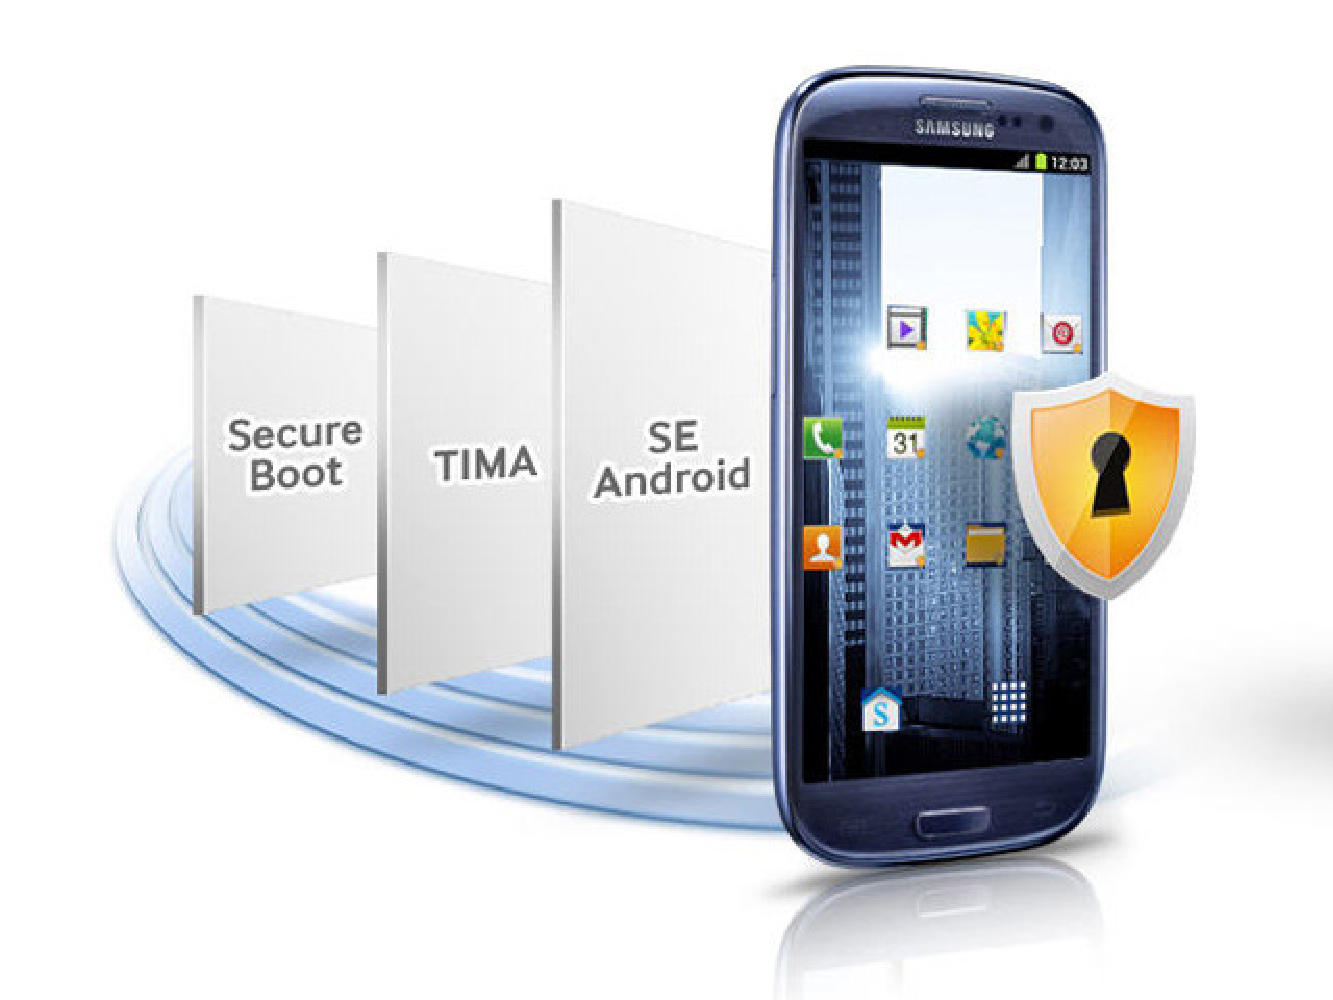
\includegraphics[scale =0.4] {gfx/byodSotA/samsung_knox.pdf}
	\caption{Samsung's Knox utility architecture. Source: \url{http://www.samsung.com/global/business/mobile/solution/security/samsung-knox}}
	\label{fig:img_knox_01}
\end{SCfigure}

Features in Blackberry Balance are similar. This security package was announced as a feature of BlackBerry 10. Nevertheless, it is available with BlackBerry Enterprise Service 10, which is a device management, security and app management for BlackBerry, iOS and Android devices. It is necessary to activate BlackBerry Balance for having available some security features, all related or similar to the aforementioned. For instance, as shown in Figure \ref{fig:blackberry_bal}, a message is displayed when the user tries to copy work data and then paste it into personal apps. Also, a user attempting for actions that are not permitted in the company ISP, or may cause secure work information to be in contact with personal applications, these actions will not be permitted. 

\begin{SCfigure}[tb]
	\centering
	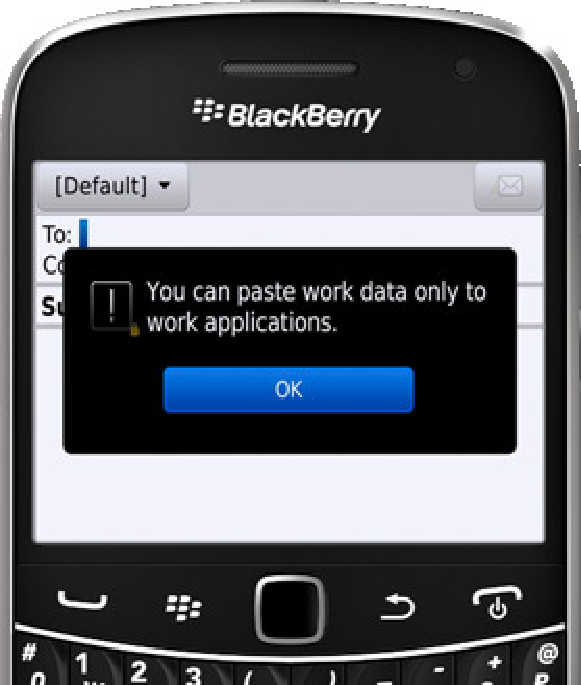
\includegraphics[scale =0.5] {gfx/byodSotA/Blackberry_balance.pdf}
	\caption{Displayed message in new Blackberry 10 when attepmting to copy sensitive company data. Source: \url{http://uk.blackberry.com/business/software/blackberry-balance.html}}
	\label{fig:blackberry_bal}
\end{SCfigure}

On the other side, while KNOX allows to \textit{push} policies from the server to the devices, so they are available offline, Blackberry Balance only allows to read documents in this mode. Finally, another known feature is also offered by Blackberry, so if the device gets lost, it is stolen, or if the employee leaves the organization, there is an option to wipe just work information which can be done remotely.

As a summary, Blackberry Balance has little opportunity if Blackberry sales continue to decrease, as well as Samsung KNOX, which is still out of the market. With this situation, MUSES could be a good choice, because is device-independent, and is available as an open source tool for both devices and servers.

%----------------------------------------------------------------------------

\subsection{Blackphone}
\label{subsec:blackphone}

On the device side, one of the most powerful solutions found in the BYOD state of the art is, apparently, to directly use a phone which has been developed with data security in mind such as the BlackPhone \cite{Blackphone}. It has its own Android-based operating system, called \textit{PrivatOS} \cite{Blackphone}, which includes a privacy-focused application store, called \textit{Silent Store}, that takes care of the problem of applications which ask for certain permissions that can lead, for instance, to personal data leakage \cite{gangula2013survey}. In Figure \ref{fig:blackphone} there is a list of the main advantages and security and privacy enhancements that PrivatOS has with respect to a standard Android OS. BlackPhone also allows a remote wiping of the data if the device is lost or stolen. The main disadvantage of this solution is either the enterprise having to make an investment and buy these smartphones to the employees or to make employees buy them, so they cannot use the device they already have. Both options are against the BYOD philosophy. On the contrary, the MUSES system proposed in this work is designed as device-independent.
Furthermore, the lack of information about this system makes it difficult to determine its real qualities.

\begin{SCfigure}[tb]
	\centering
	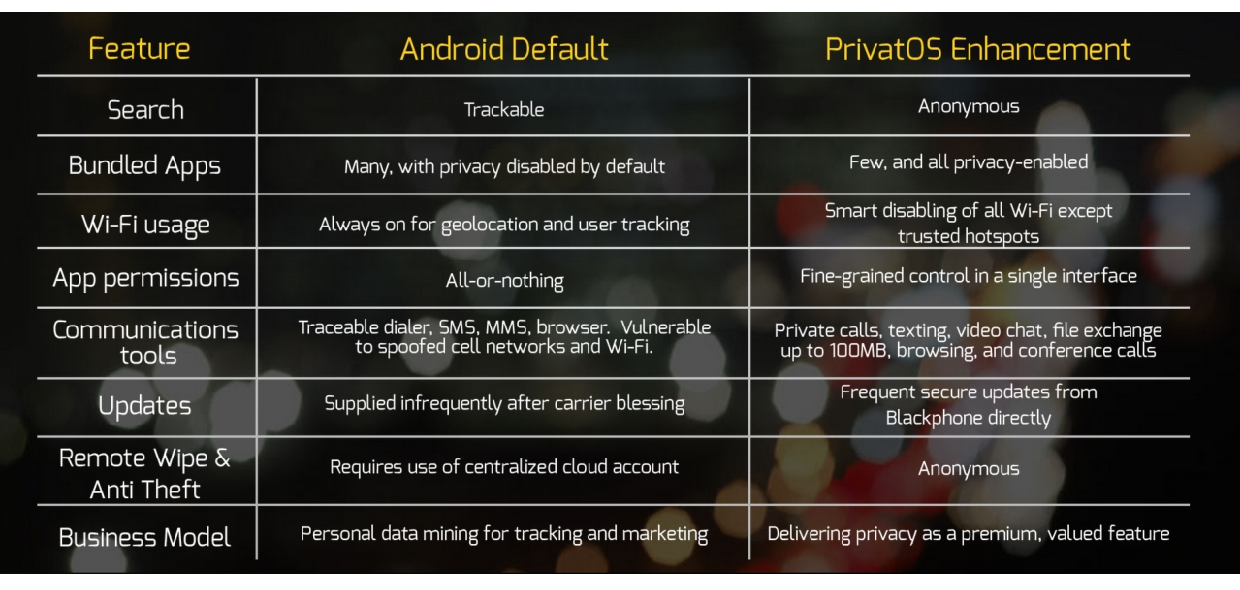
\includegraphics[scale =0.5] {gfx/byodSotA/blackphone.pdf}
	\caption{The features are compared with the ones in Android from the point of view os security and user privacy. Source: \url{https://www.blackphone.ch}}
	\label{fig:blackphone}
\end{SCfigure}

%----------------------------------------------------------------------------

\subsection{Android Work}
\label{subsec:androidwork}

This tool is the Google approach in the mobile enterprise security area, and  will run on Android 5.0 ``Lollipop''. It follows the idea of containers, previously presented in the Samsung KNOX description. Thus the container will be used to manage (encrypted) corporate data, and also to restrict what the users can do with them. This is called a ``dual-persona'' smartphone \cite{AndroidWork_review}.

This system is be strongly related to the Google Play market, as the applications will be `categorized'. Thus, Android Work provides the CSOs with a tool to define which apps would be allowed for being installed by the users and considered as corporate-related applications. Several enterprise-security aimed applications will be offered in the market, so the IT can decide which ones will be installed in the employees' devices. Also, they can manage the updates of these apps, in order to ensure that all the employees are up to date. For instance, one app could manage the creation of personal and work profiles, so the user just could access corporate assets after login in into the app. Moreover, the enterprise IT department could define specific security policies on these apps, in addition to the inherent protection that the container provides. However, the specifications of this tool \cite{AndroidWork_tool} do not include the ``self-adaptation'' as a feature, as the MUSES system does. 

Even though it does not analyze the system information for security rules evolution purposes, it offers policy management. Thus, the system will provide a framework for IT staff to manage business devices, but also, and more importantly, personal devices being used in a BYOD context. The CSO would give the employee an activation code in order to `connect' the smartphone to the enterprise and use this Android Work.
Therefore, IT admins will be able to specify which Google Play apps will be available for users to install through this work profile, including being able to provision apps to specific individuals or groups inside the company.

In addition to the work profiles, there will be considered other high-level ones with the ability to administrate the device from the corporate-security point of view, or as the owner, with all the privileges on the device.

Android Work presents only one advantage over MUSES, and roughly over all solutions, which is the ability to act over the Android kernel. The rest of tools only have permission for monitoring the running processes in the devices, while Android Work has, for instance, the ability to provide a `work' version of its native apps. MUSES, instead, depends on the developers to adapt their applications through a MUSES API, transforming them to MUSES Aware apps, as will be explained in Section \ref{subsec:client}. In any other case, and most of all with the ``self-adaptation'' feature of MUSES, it can be said that MUSES presents more advantages than the Google solution.

%----------------------------------------------------------------------------

\subsection{Multi-platform Usable Endpoint Security System}
\label{subsec:musestool}

MUSES is mainly a free, open-source, platform independent solution, and adopts the recommended best practices by Romer \cite{Romer14BestPractices}. These features make it a good alternative to most of the proprietary, close and system-specific tools presented in Section \ref{sec:toolsreview} (all but WSO2). In addition, most of the existing tools take into account only smartphones and tablets, but MUSES also covers laptops and company PCs, thus, it is not only for BYOD. Moreover, the companies which might want to work with one of the reviewed systems need a specific operating system in the server, being even more restrictive in some cases. This is specially remarkable in the case of the Blackphone, forcing the companies and the employees to purchase a specific device. MUSES is a good solution towards these cases, since it is a multi-platform system in both the client and the server.

This thesis is framed inside the European project MUSES (FP7-318508). The complete description of the MUSES project, along with the details of its architecture, can be found in Appendix \ref{chap:appendixmuses}.

%----------------------------------------------------------------------------

\subsection{Other tools}
\label{subsec:othertools}

There exist other corporate security-aimed tools inside the BYOD philosophy, of which there are less references on the Internet, but still we consider important for having similar features as MUSES. These tools are:

\subsubsection{WSO2 - Enterprise Mobility Manager}

WSO2 Enterprise Mobility Manager (WSO2 EMM) \cite{WSO2_tool} is an open source platform that also works with the BYOD program. Some of this WSO2 EMM key features are:

\begin{itemize}
  \item \textit{Mobile Device Management}: It is used to manage both user and corporate owned devices, providing support for Android and iOS at the moment. It should be noted that this tool allows tracking every enrolled device, as well as obtaining reports and analytics of their use.
  \item \textit{Mobile Application Management}: With regard to the software, this platform is able to allow or deny the use of applications on enrolled devices based on the role of the user or policies, thus restricting the use of some apps to certain users.
  \item \textit{Enterprise App Store}: This store provides users with both enterprise and public applications approved by the company.
  \item \textit{Mobile Data Security}: WSO2 also allows the user's data to be encrypted via password.
\end{itemize}

Although this tool also includes features such as device location, remote wipe, or encrypt storage, its main disadvantage is that it does not work in offline mode. In the documentation \cite{wso2Pol}, it is clearly stated that the policy compliance can be monitored while the devices are connected to the WSO2 EMM server. In addition, this tool seems to be only an MDM, without any refinement of the security policies.

\subsubsection{Good's Bring Your Own Device solution}

The philosophy followed by Good \cite{Good_tool} is similar to Samsung KNOX one: to create a secure container that places an unreachable partition between personal and business data in order to protect company assets. The solutions that they offer \cite{Good_tool} are similar than in the already described solutions. Their solution has been developed for the main OSs: iOS, Android, Windows phone, and also desktop computers with Windows. A Good's secure Network Operations Center (NOC) is introduced for dealing with the unauthorized devices, or for providing access to secure collaboration solutions (email, documents, calendar), the intranet, and both in-house or third-party mobile applications. Finally, Good offers best practice recommendations to help the company developing BYOD policies. A document can be accessed from Good's webpage \cite{Good_tool}, which contains several questions about ISPs and how to cope with all of them.

\subsubsection{Azzurri - Icon Mobilise}

It is a cloud-based service \cite{Azzurri_tool} to manage enterprise devices from the BYOD point of view, protecting sensitive corporate data and also letting the users enjoy them privately, by outsourcing the management of those devices to Azzurri.
 
\begin{itemize}
\item It offers a central deployment, administration and security control of all mobile devices regardless of their OS.
\item It manages and enforces security policies `over the air' for both corporate and employee-owned mobile devices.
\item It does it by enforcing passwords and providing mechanisms for remote lock.
\item It offers the ability to wipe, even selectively, corporate data email and contacts on the device if lost or stolen.
\end{itemize}


\subsubsection{Citrix - XenMobile}

XenMobile with the development environment called Worx App SDK, made by Citrix Systems, provides BYOD security services to companies using fine-grained policies to prevent users from performing unallowed actions \cite{WorxSDK}. For example using the mobile phone camera, GPS, or microphone. These policies can be turned on or off using its own GUI. Citrix is framework-enabled, and it is aware of the apps installed on the device. All the apps that are Worx-enabled are capable of interacting, and thus offering the user a better experience. This concept is similar to the `MUSES Aware' one, which was mentioned earlier in this section, and consists of adapting the applications to allow communications with the BYOD tools.

It is also important to point out that Citrix differentiates between apps used by the user privately and those used for business, locating both on a secure mobile container that is encrypted, and can be locked remotely for safety reasons. Another feature of Citrix is that it uses dedicated micro VPN to connect to Citrix-protected backend services.

Once the main tools and systems in this area have been introduced, in the following section our own system is presented, giving an overview on its general architecture. Moreover, we devote a subsection to describe its main features: the use of DM + ML techniques, and also its self-adaptation ability using CI methods, which compose the real difference with all the reviewed tools. 

\section{A comparison between tools}
\label{sec:comparison}

Table \ref{tab:taxonomy} summarizes the features of the main analyzed tools, with respect to the proposed taxonomy in Section \ref{sec:toolsreview}. Also, Table \ref{tab:features} shows the features of the analyzed products considering licenses, type of supported devices, and price.


\begin{SCtable}[][tb]
\resizebox{11cm}{!}{
\begin{tabular}{llllll}
\hline
\rowcolor{colorCorporativoSuave}{} & {\em \begin{tabular}[c]{@{}l@{}}Offline threat\\ detection method\end{tabular}} & {\em \begin{tabular}[c]{@{}l@{}}Updatable\\ database\end{tabular}} & {\em Standalone} & {\em \begin{tabular}[c]{@{}l@{}}Non-invasive\\ data access\end{tabular}} & {\em \begin{tabular}[c]{@{}l@{}}Superuser\\ system control\end{tabular}} \\\hline\hline
\rowcolor{colorCorporativoMasSuave}MUSES & \checkmark & \checkmark & \checkmark & \checkmark & \checkmark \\\hline
\rowcolor{colorCorporativoSuave}IBM Mobile Security &  &  & \checkmark &  &  \\ \hline
\rowcolor{colorCorporativoMasSuave}Sophos Mobile Control & \checkmark &  & \checkmark &  &  \\ \hline
\rowcolor{colorCorporativoSuave}Samsung KNOX & \checkmark &  & \checkmark & \checkmark & \checkmark \\ \hline
\rowcolor{colorCorporativoMasSuave}Blackberry Balance &  &  & \checkmark & \checkmark & \checkmark \\ \hline
\rowcolor{colorCorporativoSuave}Blackphone & - & - & \checkmark & \checkmark & \checkmark \\ \hline
\rowcolor{colorCorporativoMasSuave}Android for Work & \checkmark &  & \checkmark & \checkmark & \checkmark \\ \hline\hline
\end{tabular}
}
\caption{Features of the analysed tools with regard to the proposed taxonomy to classify BYOD systems.}
\label{tab:taxonomy}
\end{SCtable}

\begin{SCtable}[][tb]
\resizebox{11cm}{!}{
\begin{tabular}{llll}
\hline
\rowcolor{colorCorporativoSuave}{} & {\em License} & {\em Devices} & {\em Price} \\\hline\hline
\rowcolor{colorCorporativoMasSuave}MUSES & OpenSource & \begin{tabular}[c]{@{}l@{}}Android, iOS,\\Windows 8.1,\\Windows Phone\end{tabular} & Free \\\hline
\rowcolor{colorCorporativoSuave}IBM Mobile Security& Proprietary & \begin{tabular}[c]{@{}l@{}}Android, iOS,\\Windows Phone,\\Blackberry\end{tabular} & By request \\ \hline
\rowcolor{colorCorporativoMasSuave}Sophos Mobile Control & Proprietary & \begin{tabular}[c]{@{}l@{}}Android, iOS,\\Windows Phone\end{tabular} & By request \\ \hline
\rowcolor{colorCorporativoSuave}Samsung KNOX & Proprietary & \begin{tabular}[c]{@{}l@{}}Android, iOS,\\Samsung devices\end{tabular} & \begin{tabular}[c]{@{}l@{}}12\$ per\\year/device\end{tabular} \\ \hline
\rowcolor{colorCorporativoMasSuave}Blackphone & Proprietary & Own device & 120\$ per year \\ \hline
\rowcolor{colorCorporativoSuave}Android for Work & Proprietary & \begin{tabular}[c]{@{}l@{}}Android,\\devices with\\Chrome browser\end{tabular} & \begin{tabular}[c]{@{}l@{}}12\$ per\\month/user\end{tabular} \\ \hline\hline
\end{tabular}
}
\caption{Features of the analysed products considering licenses, type of devices and OS, and price..}
\label{tab:features}
\end{SCtable}


Another comparison would be that the existing products are mostly policy-based, while MUSES makes its decisions not only considering policies, but also based on the terminals and users context, such as connection properties, or trust value of the device, to really understand the real risk that comes with a specific action.

Also related to this issue, a very big advantage of the MUSES system that is not present in the other solutions is its self-adaptivity power. The proposed system uses different methods to create new security rules, being their aim to cover new vulnerabilities or threats. Thus, MUSES is able to adapt to changes by applying classification techniques to create new rules, and then refining the whole set of existing policies. Additionally, MUSES is able to discover new threats by a combination of real-time risk and trust analysis plus a classifier trained with all the occurred events in the system.

However, MUSES presents a limitation regarding the enhance of rules, since, in principle, it cannot predict or generate rules for dealing
with unexpected or unknown events, which could lead to a security incident. The philosophy is that the initial set of rules, defined by the CSO, should be very restrictive regarding possible unexpected users' behaviours or events, in order to avoid as much security incidents as possible. As the system works, MUSES would be able to define new rules through refinement which could get an associated decision after the corresponding events have happened. Thus, this will lead to obtaining an optimal set of security rules.

In addition, MUSES can also infer or create new rules using computational intelligence techniques. These rules could deal with unexpected situations not previously happened, but must be previously approved by the CSO. Of course, everything is constrained by the available set of sensors which, in turn, define the possible information that MUSES will analyze and use in the refinement and inference processes.

Moreover, another clear improvement over the rest is that MUSES can work in both online and offline modes, depending on the client being able to connect with the server or not, which favours the real-time decision making process.

These are not only advantages of MUSES over the existing products, but also a progress beyond the state of the art in some fields like risk and trust analysis, event correlation, and human-computer interaction (HCI).

First, as mentioned previously, it  implements a self-adaptive event correlation, including a novel hybrid technique of rule refinement and rule adjustment extracting relevant information from processing huge amounts of data. Then, the project defines a new approach to risk management taking into account threats, with their costs, as well as the innovative concept of opportunity: the following beneficial outcome from a situation on which, for instance, a user is able to work while waiting at the airport if the risk is low enough. 

As far as the HCI is concerned, in Section \ref{sec:preliminaryconcepts} we talked about how it has been demonstrated by Shaw et al. \cite{SecPolComp09} and Herath et al. \cite{SecPolPenalty09} that the compliance of the employees of a company, with respect to the security policies, increases by educating them and decreases by punishing them. Therefore, the fact that MUSES is focused in avoiding security incidents due to users' unawareness of the ISPs, it sets up a significant advance in the state of the art. This is because not only the incident is avoided, but the user is educated, which at the same time avoids future risky situations.
With regard to device monitoring, MUSES  also take into account the so-called context observation, by which private or professional scenarios can be detected, or predicted, based on advanced machine learning techniques. Finally, the project is concerned about legal compliance in regards of Information Security Policies, so that it  contributes to the proposal for the EU Data Protection: legal binding force and legal certainty of company policies, and end-user responsibility.

With regard to the scientific contribution of the system, one of the main differences with respect to previous works is the consideration of security threats `brought' by the user's behavior inside the system, i.e. through interaction or events, rather than more general and external threats. Moreover, the techniques to be used in MUSES  works with real data, as a difference to several research works which consider simulated data.

Authors have used DM techniques in previous works, but usually aiming for a specific general objective, for instance the detection of threats such as botnet \cite{botnet_detection_clustering_09}, or the recognition of anomalies \cite{feature_selection_anomalies_08}. However, these works do not contemplate any process to improve the system as the refinement phase in MUSES.

There are some proposals in which security policies are inferred or refined \cite{inferring_policies_socialnetworks_09,policy_generation_clustering_10}, but they do not affect the ISPs as in MUSES, and they are not based on the user's behaviour in order to do this.

GP has been previously proposed in bibliography \cite{rule_generation_gp_09,sec_policy_evolution_gp_08}, even for creating new policies or rules in a security-aimed sense. In any case they do not affect the ISPs and moreover, our proposed evaluation functions, completely integrated in the system, for the refinement and inference approaches are novel.

With respect to GA, they have been extensively used in this scope in the literature, mainly for the detection of anomalies and intrusions rather than for optimization, as it is used in the proposed system. However, there are some examples that could be used as model for our approach, such as \cite{EAs_securitycosts-kirta,risk_reduction_ga_12}.
}{\myChapter{Corporate Security Solutions for BYOD}\label{chap:byodSotA}}
%%\ifthenelse{\equal{\value{IncluyeCapitulo}}{5}}{\include{Chapters/BajaVision}}{\myChapter{Cuestionarios para la \textsc{Baja Visi�n}}\label{sec:cuestionariosBajaVision}}
%%-----------------------------
\myPart{Materials and Methods}\label{part:metodoYmateriales}
\ifthenelse{\equal{\value{IncluyeCapitulo}}{2}}{\myChapter{Applied methods... title TBC}\label{chap:softc} 
\chaptermark{Applied methods... title TBC} 

\begin{flushright}{\slshape
    ...} \\ \medskip
    --- {}
\end{flushright}

\minitoc\mtcskip
\vfill

\lettrine{S}{ince} the final outcome from the application of the methodology that is proposed in this thesis is a set of rules, that will aid the CSOs in the process of reviewing and extending the set of security policies, we present the most suitable techniques to produce this outcome, taking into account the input data. The input data are be the actions that the employees make with their devices in certain situations, hence the final problem is that of classification, to see if they should be allowed or not.

Therefore, in this chapter we will look over the techniques that take part in the process, from selecting the data in the database to actually obtaining the set of rules and visualise them, via data preprocessing and transformation. Furthermore, the soft computing techniques that have been applied in research for the problem of classification -- extraction of rules -- and visualisation are also detailed.

It is important to note that this process, known as ``Knowledge Discovery in Databases'' is not the proposed methodology itself, but part of it. These are the necessary steps and methods to obtain the rules, but the proposed algorithms can be used or not depending on the use case, which will be defined later.

\section{The Knowledge Discovery in Databases process}

The process of discovering new -- previously unknown or non trivial -- relationships between the instances of the data, being these the observations of the use case in certain environments, has been named ``Knowledge Discovery in Databases'' or KDD \cite{fayyad1996data}. Every step of the process is described in \cite{fayyad1996data}, where the authors also remark that the Data Mining procedure is part of KDD. This is because even though DM is the most famous and indeed is a very importante step, the rest are equally important and sometimes more, because without a proper preprocessing or interpretation of the results, DM could lead to misunderstandings.

This way, the steps detailed in \cite{fayyad1996data} are the following:

\begin{enumerate}
	\item Identifying the desired outcome or use of the process by the final user.
	\item Obtaining the set of data to explore.
	\item Cleaning and preprocessing of the data.
	\item Transforming the data in order to obtain new attributes of the observations or reduce them.
	\item Identifying the methods to use according to what has been defined in step 1.
	\item Applying the methods.
	\item Presenting the results in a suitable way for the final user.
\end{enumerate}

In the succeeding sections, we will describe the most used techniques for every case.

\section{Data selection}

When we talk about selecting the target data, we refer to choosing the set of data to which we want to apply the different, either if is the whole set of observations or a subset of it. The reasons for using all the data at hand or just a portion will entirely depend on the aim of the use case, and whether we want to generaly discover new relationships between the observations or just to study a particular group or time of day. For this reason, there is not a particular technique that can be used in this step, as it consists of gathering the data from the source of the observations.

Therefore, this is a matter of properly designing the database, and it is more important to do so for scalability reasons, when the number of observations that will be stored tend to be treated the same way as ``Big Data'' \cite{begoli2012design, wu2014data}.

\section{Data preprocessing}

The preprocessing of the data includes the treatment of some of the values, the cleaning of the database, and the application of balancing techniques.

On the one hand, the data might not be directly stored in the way that it is needed for the knowledge discovery. This means that either the information is in log files from what the observations have to be extracted and stored in a database, or even if the data is already in a database, the attributes related with the observation might be distributed along many different tables. What is more, the assignation of a \textit{class}, i.e. a label which describes the group to which an observation belongs, can be made manually or by performing techniques such as clustering \cite{witten2016data}. In addition, new attributes can be added to the observation by processing the ones obtained directly from the sensor, and this way we add information that might be helpful. Then, this preprocessing and actual making of the dataset is an adaptable task, because it can be done with any chosen tool. However, this is a process that can be avoided with a careful definition of the values of interest and the structure of the database that will store them.

On the other hand, the observation of the real world can lead to missing or repeated values due to failing sensors or the communication with them. This is why it is important to perform a database cleaning. The work discussed in \cite{wilson2001maintaining} presents an exhaustive review of works which study database cleaning and their conclusion is that a database with good quality is decisive when trying to obtain good accuracies when classifying new observations; a fact which was also demonstrated in \cite{zeineb2014thesis}. This means that the model that will be built in the data mining step will be more helpful, and more knowledge can be extracted, when the database is well maintained.

Many cleaning techniques have been proposed in literature \cite{wilson2001maintaining} in order to guarantee the good quality of
a given dataset. Most of these techniques are based on updating a database by adding or deleting instances to optimize and reduce the initial database. These policies include different operations such as deleting the outdated, redundant, or inconsistent instances; merging groups of objects to eliminate redundancy and improve reasoning power; re-describe objects to repair incoherencies; check for signs of corruption in the database and controlling any abnormalities in the database which might signal a problem. Working with a database which is not cleaned can become sluggish and without accurate data users will make uninformed decisions.

Lastly, it is also usual to have an unequal number of observations in every class or group. This is called ``data imbalance'' \cite{imbalanced_data_05}. In order to deal with this problem there exist several methods in the literature, but all of them are mainly grouped in three techniques \cite{imbalance_techniques_02}: 

\begin{itemize}
\item \textit{Undersampling the majority classes}: i.e. reduce the considered number of patterns for the classes with the majority.
\item \textit{Oversampling the minority classes}: i.e. introduce additional -- normally synthetic -- patterns in the classes with the minority.
\item \textit{Modifying the cost associated to misclassifying the positive and the negative class} to compensate for the imbalance ratio of the two classes. For example, if the imbalance ratio is 1:10 in favour of the negative class, the penalty of misclassifying a positive example should be 10 times greater.
\end{itemize}

The first option has been applied in some works, following a random undersampling approach \cite{random_undersampling_08}, but it has the problem of the loss of valuable information. 
% dónde está la primera hand? - JJ
The second has been so far the most widely used, following different approaches, such as SMOTE (Synthetic Minority Oversampling Technique) \cite{smote_02}, a method proposed by Chawla et al. for creating ``artificial'' samples for the minority class, in order to balance the amount of them with respect. However this technique is based in numerical computations, which consider different distance measures, in order to generate useful patterns , i.e. realistic or similar to the existing ones.

The third option implies using a method in which a cost can be associated to the classifier accuracy at every step. This was done for instance by Alfaro-Cid et al. in \cite{cost_adjustment_07}, where they used a Genetic Programming (GP) approach in which the fitness function was modified in order to consider a penalty when the classifier makes a false negative -- an element from the minority class was classified as belonging to the majority class --. However almost all the approaches deal with numerical data, which is important to take into account when working with nominal -- not integer or real -- values as well.

\section{Data transformation}



\section{Soft computing techniques applied to data mining and visualisation}

Until now, for the other parts of the process, we have focused in some characteristics of the dataset, such as the number of attributes, whether it has missing values, or the difference between cases belonging to each class. But the type of data for every attribute is also important, because it will determine the kind of algorithms that can be used.

This way, an attribute can be \textit{numeric} or \textit{nominal} \cite{witten2016data}. Numeric attributes measure continuous values such as integers and real numbers, and boolean as well, whilst nominal attributes -- also named \textit{categorical} -- take their value from a predefined, finite set of possibilities. In what follows we will overview the algorithms that can be used in the cases that, like ours, the data is mostly nominal.

\subsection{Classification in the data mining process}

Inside KDD, the process of classification, or application of classifying algorithms, helps in building a model of the data set, and to understand the relationships therein. As previously said, the data coming from BYOD practises is usually not only numerical or nominal, thus, only classification algorithms that support both types of data can be considered. Weka \cite{weka:site} is a collection of State-of-the-Art machine learning algorithms and data preprocessing tools that are key for data mining processes \cite{witten2016data}. On the other hand, it is important that for our purposes we focus on rule-based and decision-tree-based algorithms. A decision-tree algorithm is a group of conditions organised in a top-down recursive manner in a way that a class is assigned following a path of conditions, from the root of the tree to one of its leaves. Generally speaking, the possible classes to choose are mutually exclusive. Furthermore, these algorithms are also called ``divide-and-conquer'' algorithms. On the other hand, there are the ``separate-and-conquer'' algorithms, which work creating rules one at a time, then the instances covered by the created rule are removed and the next rule is generated from the remaining instances. The most important characteristic of these algorithms is that the model that is built from the dataset is expressed in the form of a set of rules.

Inside the rule-based and decision tree-based algorithms, there is a great number of possible algorithms to work with, we have conducted a preselection phase trying to choose those which would yield better results in the experiments. A reference to each Weka classifier can be found at \cite{witten2016data}. Below are described the top five techniques, obtained from the best results  of the experiments done in this stage, along with more specific bibliography. Na\"{i}ve Bayes method \cite{Bayesian_Classifier_97} has been included as a baseline, normally used in text categorization problems. According to the results, the five selected classifiers are much better than this method.

\begin{description}
  \item[Na\"{i}ve Bayes] It is the classification technique that we have used as a reference for either its simplicity and ease to understand. Its basis relies on the Bayes Theorem and the possibility of represent the relationship between two random variables as a Bayesian network \cite{rish2001empirical}. Then, by assigning values to the variables probabilities, the probabilities of the occurrences between them can be obtained. Thus, assuming that a set of attributes are independent one from another, and using the Bayes Theorem, patterns can be classified without the need of trees or rule creation, just by calculating probabilities.
   \item[J48] This classifier generates a pruned or unpruned C4.5 decision tree. Described for the first time in 1993 by \cite{Quinlan1993}, this machine learning method builds a decision tree selecting, for each node, the best attribute for splitting and create the next nodes. An attribute is selected as `the best' by evaluating the difference in entropy (information gain) resulting from choosing that attribute for splitting the data. In this way, the tree continues to grow till there are not attributes anymore for further splitting, meaning that the resulting nodes are instances of single classes. 
   \item[Random Forest] This manner of building a decision tree can be seen as a randomization of the previous C4.5 process. It was stated by \cite{Breiman2001} and consist of, instead of choosing `the best' attribute, the algorithm randomly chooses one between a group of attributes from the top ones. The size of this group is customizable in Weka.
   \item[REP Tree] Is another kind of decision tree, it means Reduced Error Pruning Tree. Originally stated by \cite{Quinlan1987}, this method builds a decision tree using information gain, like C4.5, and then prunes it using reduced-error pruning. That means that the training dataset is divided in two parts: one devoted to make the tree grow and another for pruning. For every subtree (not a class/leaf) in the tree, it is replaced by the best possible leaf in the pruning three and then it is tested with the test dataset if the made prune has improved the results. A deep analysis about this technique and its variants can be found in \cite{Elomaa2001}.
   \item[NNge] Nearest-Neighbor machine learning method of generating rules using non-nested generalised exemplars, i.e., the so called `hyperrectangles' for being multidimensional rectangular regions of attribute space \cite{Martin1995}. The NNge algorithm builds a ruleset from the creation of this hyperrectangles. They are non-nested (overlapping is not permitted), which means that the algorithm checks, when a proposed new hyperrectangle created from a new generalisation, if it has conflicts with any region of the attribute space. This is done in order to avoid that an example is covered by more than one rule (two or more).
   \item[PART] It comes from `partial' decision trees, for it builds its rule set from them \cite{Frank1998}. The way of generating a partial decision tree is a combination of the two aforementioned strategies ``divide-and-conquer'' and ``separate-and-conquer'', gaining then flexibility and speed. When a tree begins to grow, the node with lowest information gain is the chosen one for starting to expand. When a subtree is complete (it has reached its leaves), its substitution by a single leaf is considered. At the end the algorithm obtains a partial decision tree instead of a fully explored one, because the leafs with largest coverage become rules and some subtrees are thus discarded.
 \end{description} 

\subsection{Data visualisation and interpretation}}{\myChapter{Soft computing techniques applied to classification}\label{chap:softc}}
\ifthenelse{\equal{\value{IncluyeCapitulo}}{2}}{\myChapter{A methodology for obtaining rules in BYOD environments}\label{chap:methodology}


\begin{flushright}{\slshape
    ... } \\ \medskip
    --- {}
\end{flushright}

\minitoc\mtcskip
\vfill
\lettrine{}{}

%The steps of the methodology are:
%
%Use case identification
%Data identification
%Analysis
%Establishing desirable metrics
%Applying the most suitable SC techniques

%\section{Scenarios}
%\label{sec:scenarios}
%
%\section{Analysis on the attributes}
%\label{sec:attributes}}{\myChapter{A methodology for obtaining rules in BYOD environments}\label{chap:methodology}}
%%\ifthenelse{\equal{\value{IncluyeCapitulo}}{8}}{\include{Chapters/cuestionariosBordes}}{\myChapter{Recomendaciones para la Construcci�n de Cuestionarios de calidad de bordes}\label{chap:recCuestCalidadBordes}}
%%-----------------------------
\myPart{Experimental Results}\label{part:resultadosExperimentales}
\ifthenelse{\equal{\value{IncluyeCapitulo}}{2}}{\myChapter{Going a Step Beyond the Black and White Lists for URL Accesses in the Enterprise by Means of Categorical Classifiers}\label{chap:urls}

\begin{flushright}{\slshape
  ...} \\ \medskip
    --- {}
\end{flushright}

\minitoc\mtcskip
\vfill

\lettrine{E}{very} section corresponds to a step in the methodology.


\section{Use case identification}

The CSPs usually include policies that allow or deny access to non-confident (or non-certified) web sites. Moreover, several web pages might be also controlled for productivity or suitability reasons. Thus, some of the CSPs usually define sets of allowed or denied pages/sites that could be accessed by the enterprise users/employees. These sets are usually included in a White (permitted) or Black (non-permitted) Lists. These lists act as a good control tool for those URLs included in them of for the complementary, i.e. the URLs not included in a Whitelist have automatically denial of access, for instance.

The aim is going a step beyond, trying to define a tool for automatically making an allowance or denial decision with respect to URLs that are not included in the aforementioned lists. This decision would be based in the one made for similar URL accesses (those with similar features).

Thus, the problem has been transformed into a \textit{classification} one, in which we have started from a set of unlabelled patterns, that model the connection properties from a huge amount of \textit{real}\footnote{Taken from a log file given by a volunteer Spanish company.} URL accesses (known as sessions). Then we have assigned a label to many of them, considering a set of \textit{real}\footnote{The set of rules has been written by the same company, with respect to its employees.} security rules (CSPs) defined by the Chief Security Officer (CSO) in the company.
The resulting dataset has been processed by means of different classification methods, in order to find the best algorithm for dealing with these data.
Previously, data balancing techniques were applied, namely \textit{undersampling} and \textit{oversampling} \cite{imbalance_techniques_02}, due to the high imbalance present in the dataset, given that more than two thirds of the patterns belonged to the majority class.

The problem to solve is related with the application of corporate security policies in order to deal with potential URL accesses inside an enterprise. To this end a dataset of URL sessions (requests and accesses) is analysed. These data are labelled with the corresponding permission or not for that access following the aforementioned rules. The problem is then transformed into a classification one, in which every new URL request will be classified, and thus, a grant or deny action will be assigned to that pattern.

The analysed data come from an \texttt{access.log} of the Squid proxy application \cite{squid:site}, in a real Spanish company. This open source tool works as a proxy, but with the advantage of storing a cache of recent transactions so future requests may be answered without asking the origin server again \cite{DuaneWessels2004}. Every pattern, namely a URL session has ten variables associated, which we describe in Table \ref{tabdata}, indicating if the variable is numeric or nominal/categorical.

\begin{table*}[htpb]
\centering
 \caption{\label{tabdata} Independent Variables corresponding to a URL session (a connection to a URL for some time). The URLs are parsed as detailed in Section \ref{sec:dataid}.}
{\scriptsize
\begin{tabular}{llll}
\hline\noalign{\smallskip}
Variable name & Description & Type & Rank/Number of Values (if categorical)\\
\noalign{\smallskip}\hline\noalign{\smallskip}
\texttt{http\_reply\_code} & Status of the server response & Categorical & 20 values\\
\texttt{http\_method} & Desired action to be performed & Categorical & 6 values\\
\texttt{duration\_milliseconds} & Session duration & Numerical & integer in [0,357170]\\
\texttt{content\_type} & Media type of the entity-body sent to the recipient & Categorical & 11 values (main content), 85 values (whole content)\\
\texttt{server\_or\_cache\_address} & IP address & Categorical & 2343 values\\
\texttt{time} & connection hour (in the day) & Date & 00:00:00 to 23:59:59\\
\texttt{squid\_hierarchy} & It indicates how the next-hop cache was selected & Categorical & 3 values\\
\texttt{bytes} & Number of transferred bytes during the session & Numerical & integer in [0,85135242]\\
\texttt{client\_address} & IP address & Categorical & 105 values\\
\texttt{URL} & Core domain of the URL, not taking into account the TLD & Categorical & 976 values\\
%\noalign{\smallskip} \hline\noalign{\smallskip}
%Non-financial Variables (used in GP) & Description & Type\\
%\noalign{\smallskip}\hline\noalign{\smallskip}
%$x_0$, $x_1$, $x_2$ & Size & Small/Medium/Large& Categorical\\
\noalign{\smallskip}\hline
\end{tabular}
}
\end{table*}

The dependent variable or class is a label which inherently assigns an decision (and so the following action) to every request. This can be: \textit{ALLOW} if the access is permitted according to the CSPs, or can be \textit{DENY}, if the connection is not permitted. These patterns are labelled using an `engine' based in a set of security rules, that specify the decision to make.

These data were gathered along a period of two hours, from 8.30 to 10.30 am (30 minutes after the work started), monitoring the activity of all the employees in a medium-size Spanish company (80-100 people), being 100000 patterns. The results derived from the experiments show that this quantity of data might be big enough, but a more accurate outcome would be given with, for instance, a 24 hours long log.

\section{Data identification}
\label{sec:dataid}

Before classification techniques are applied, a data preprocessing step has been performed. First, the raw dataset is labelled according a set of \textit{initial corporate security rules}, i.e. every pattern is assigned to a label indication if the corresponding URL request/access would be ALLOWED or DENIED considering these rules. This step is necessary in order to transform the problem into a classification one. However, in order to apply the rules they must be transformed from their initial format into another one that can be applied in our programs (a hash in Perl\footnote{A \textit{hash} in Perl is an object that represents a \textit{hash table}, which is a set of pairs key-value. Sometimes, the value can be another hash itself.}). This is described in Subsection \ref{subsec:ruleparsing}. 

Subsection \ref{subsec:logparsing} details how the patterns of the navigation data log (URL sessions) are also converted to a Perl hash to perform the matting/labelling process. 

At the end of these two steps, the two hashes are compared in order to obtain which entries of the log should be ALLOW or DENY, know as the \textit{labelling} step. This is similar to perform a decision process in a security system. This step results in that there are 38972 pattern belonging to class ALLOW (positive class) and 18530
of class DENY (negative class), so just a 67.78\% of the samples
belong to the majority class. This represents a very important problem, since a classifier that is trained considering these proportions is supposed to classify all the samples as ALLOW, getting a theoretically
quite good classification accuracy equal or greater than 68\%. However, in section \ref{sec:results} we will see that, despite the fact that some denied patterns are classified as allow, the overall performance of the classifiers are better than the expected.% Eso
                                % no es bueno. Es una mierda - JJ
Given that the dataset contains a majority of categorical/nominal data, we have performed different approaches for data balancing:
\begin{itemize}
\item Undersampling: we will remove random samples of the majority class until the amount in both classes are similar.
\item Oversampling: we will duplicate random samples of the minority class, in order to get a close number of patterns in both classes. This has be done due to the impossibility of creating synthetic data when dealing with categorical values (there is not a proper distance measure between two values in a category). Actually, since the number of samples in the majority class is almost twice the minority one, we have just duplicated all of those belonging to the minority class.
\end{itemize}

Finally, in Subsection \ref{subsec:methods} we explain the selection of the methods to apply in order to classify the data. We just have considered the patterns correctly labelled in the preprocessing phase. Thus, a supervised classification process \cite{classification_67} has been conducted on the balanced datasets.
Weka Data Mining Software\footnote{http://www.cs.waikato.ac.nz/ml/weka/} has been used, in order to select the best set of methods in order to deal with these data. These classifiers will be further tested in Section \ref{sec:results}.

% ------------------------------------------------------------------
%
\subsection{Security rules parsing}
\label{subsec:ruleparsing}

\noindent In this work we have considered Drools \cite{drools:site}
as % otra cosa que debería estar en el estado del arte.  - JJ
the tool to create and therefore manage rules in a business environment. This so called Business Rule Management System (BRMS) has been developed by the JBoss community under an Apache License and it is written in Java. Though this platform consist of many components, here we focus on Drools Expert and the Drools Rule Language (DRL, \cite{drools:doc}). Then, the defined rules for a certain company are inside of a file with a \texttt{.drl} extension, the file that needs to be parsed to obtain the final set of rules. In Figure \ref{fig:drools_hash}, (a), there is the typical rule syntax in DRL. Two main things should be obtained from the parsing method: both left and right sides of the rule, taking into account that the left side is where the company specifies the conditions required to apply the action indicated in the right side. Also, for describing the conditions, Squid syntax is used (see Section \ref{sec:problemDescription}), having thus the following structure: \texttt{squid:Squid(\textit{conditions})}. Finally, from the right side of the rule, the \textit{ALLOW} or \textit{DENY} label to apply on the data that matches with the conditions, will be extracted. The Perl parser that we have implemented applies two regular expressions, one for each side of the rule, and returns a hash with all the rules with the conditions and actions defined. The `before and after' performing the parsing over the \texttt{.drl} file is in Figure \ref{fig:drools_hash}.

\begin{figure}[htb]
\centering
\subfloat[Drools Rule]{
\begin{tabular}{ p{0.05cm} p{0.05cm} p{2.5cm} }
  \texttt{rule~"name"} & & \\
   & \texttt{attributes} & \\
   & \texttt{when} & \\
   & & \texttt{/* Left Side of the Rule */} \\
   & \texttt{then} & \\
   & & \texttt{/* Right Side of the Rule */} \\
  \texttt{end} & & \\
\end{tabular}
}
~
\subfloat[Hash Rule]{
\begin{tabular}{ p{0.05cm} p{0.05cm} p{2.5cm} }
  \texttt{\%rules~=~(} & & \\
   & \texttt{rule~=>\{} & \\
   & & \texttt{field => xxx} \\
   & & \texttt{relation => xxx} \\
   & & \texttt{value => xxx} \\
   & & \texttt{action => [allow, deny]} \\
   & \texttt{\},} & \\
  \texttt{);} & & \\
\end{tabular}
}
\caption{(a) Structure of a rule in Drools Expert. (b) Resulting rule, after the parsing, in a global hash of rules. \label{fig:drools_hash}}
\end{figure}

% ------------------------------------------------------------------
%
\subsection{URL log data parsing}
\label{subsec:logparsing}

\noindent Usually, the instances of a log file have a number of fields, in order to have a registration of the client who asks for a resource, the time of the day when the request is made, and so on. In this case, we have worked with an \textit{access.log} (see Section \ref{sec:problemDescription}) file, converted into a CSV format file so it could be parsed and transformed in another hash of data. All ten fields of the Squid log yield a hash like the one depicted in Figure \ref{fig:data_hash}.

Once the two hashes of data were created, they were compared in such a way that for each rule in the hash of rules, it was determined how many entries in the data log hash are covered by the rule, and so they were applied the label that appears as `action' in the rule.

One of the problems was to extract from a whole URL the part that was
more interesting for our purposes. It is important to point out that
in a log with thousands of entries, an enormous variety of URLs can be
found, since some can belong to advertisements, images, videos, or
even some others does not have a domain name but are given directly by
an IP address. For this reason, we have taken into account that for a
domain name, many subdomains (separated by dots) could be considered,
and their hierarchy grows from the right towards the left. The highest
level of the domain name space is the Top-Level Domain (TLD) at the
right-most part of the domain name, divided itself in country code
TLDs and generic TLDs. Then, a domain and a number of subdomains
follow the TLD (again, from right to left). This way, the URLs in the
used log are such as \textit{http://subdomain...subdomain.domain.TLD/}
\textit{other\_subdirectories}. However, for the ARFF\footnote{Format
  of Weka files} file to be created, only the domain (without the
subdomains and the TLD) should be considered, because there are too
many different URLs to take into consideration. Hence, applying
another regular expression, the data parser implemented in Perl
obtains all the core domains of the URLs, which makes 976 domains in
total. % primero: deberíais usar domain + TLD. Perl.com no es lo mismo
       % que perl.org. Segundo: deberíais de justificar esto un poco
       % más. Pensaba que usábais algo más avanzado para clasificar el
       % sitio, directorios o algo... - JJ

\begin{figure}[htb]
\centering
\caption{Perl hash with an example entry. The actual hash used for this work has a total of 100000 entries, with more than a half labelled as \textit{ALLOW} or \textit{DENY} after the comparing process. \label{fig:data_hash}}
\begin{tabular}{ p{0.1cm} p{0.1cm} p{6cm} }
  \texttt{\%logdata~=~(} & & \\
   & \texttt{entry~=>\{} & \\
   & & \texttt{http\_reply\_code => xxx} \\
   & & \texttt{http\_method => xxx} \\
   & & \texttt{duration\_miliseconds => xxx} \\
   & & \texttt{content\_type => xxx} \\
   & & \texttt{server\_or\_cache\_address => xxx} \\
   & & \texttt{time => xxx} \\
   & & \texttt{squid\_hierarchy => xxx} \\
   & & \texttt{bytes => xxx} \\
   & & \texttt{url => xxx} \\
   & & \texttt{client\_address => xxx} \\
   & \texttt{\},} & \\
  \texttt{);} & & \\
\end{tabular}
\end{figure}


\section{Analysis}


\section{Establishing desirable metrics}


\section{Applying the most suitable soft computing techniques}

Several experiments have been conducted, once a subset of classification methods has been chosen in previous section.
To this end, some training and test datasets have been created from the set of labelled patterns. It contains 57502 samples, with 38972 belonging to class ALLOW and 18530 to class DENY.

In order to better test the methods, two different divisions (training-test) have been done, namely 90\%-10\% and 80\%-20\%. Moreover, two additional splits have been considered in every case, using both a random and a sequential approach for selecting samples from the original file. Thus, in the latter, consecutive patterns have been included in the training file up to the desired percentage. The rest have composed the test file. In the first approach, a random selection is performed.

The aim of the sequential division is to compare if the online activity of the employees considering URL sessions could be somehow `predicted', just using data from previous minutes or hours.

With respect to the data, the initial file was unbalanced, as it can be seen in the number of patterns per class. Hence, as stated in Section \ref{sec:problemDescription}, two data balancing methods have been applied to all the files, to get similar numbers in both classes: undersampling (random removal of ALLOW patterns) and oversampling (duplication of DENY patterns).

Results for unbalanced data are presented in Table \ref{tabresults_nobalan}.
Three different tests have been done for the random pattern distribution approach, so the mean and standard deviation are shown in the corresponding columns.

\begin{table*}[htpb]
\centering
 \caption{\label{tabresults_nobalan} Percentage of correctly classified patterns for non-balanced data}
{\small
\begin{tabular}{|l|l|l|l|l|}
\cline{2-5}
\multicolumn{1}{l|}{} & \multicolumn{2}{c|}{80\% Training - 20\% Test} & \multicolumn{2}{c|}{90\% Training - 10\% Test} \\ 
\cline{2-5}
\multicolumn{1}{l|}{} & Random (mean) & Sequential & Random (mean) & Sequential \\ 
\hline
J48 & 97.56 $\pm$ 0.20 & 88.48 & 97.70 $\pm$ 0.15 & 82.28 \\ 
\cline{1-1}
Random Forest & 97.68 $\pm$ 0.20 & 89.77 & 97.63 $\pm$ 0.13 & 82.59 \\ 
\cline{1-1}
REP Tree & 97.47 $\pm$ 0.11 & 88.34 & 97.57 $\pm$ 0.01 & 83.20 \\ 
\cline{1-1}
NNge & 97.23 $\pm$ 0.10 & 84.41 & 97.38 $\pm$ 0.36 & 80.34 \\ 
\cline{1-1}
PART & 97.06 $\pm$ 0.19 & 89.11 & 97.40 $\pm$ 0.16 & 84.17 \\ 
\hline
\end{tabular}
}
\end{table*}
% primero: ¿las diferencias son significativas? No lo
% parecen. Segundo: ¿habéis incluido algún método "baseline" para
% comparación, como NaiveBayes, que es el que se incluye siempre? - JJ 
As it can be seen, all the five methods achieved a high performance classifying in the right way the test dataset. Also, these results are not like this by chance, as shown by a low standard deviation. Although it was expected that the results from the 90\%-10\% division were slightly better, in the future a more agressive division will be executed so the methods can be really proved with much less training data.

What matters to the results of the experiments made with the sequential data, they are worse than the obtained from the random data, but still they are good ($>$ 85\%). This is due to the occurrence of new patterns from a certain time (maybe there are some requests that are made just at one specific time in a day, or in settled days), and then there is no sufficient similarity between the training data and the classifying of the test data set may fail. The loss of 5 to 6 points in the results of the 90\%-10\% division is the first unexpected or unlogicall result of the experiments, but they also reinforce the previous theory.

The technique that lightly stands out over the others is
\textit{Random Forest}, being the best in almost every case, even in
the experiments with the most complex sequential divisions. However,
if we focus on the standard deviation, \textit{REP Tree} is the chosen
one, as its results present robustness. % yo no estaría tan
                                % seguro. Tenéis que hacer tests
                                % estadísticos. En serio que parecen
                                % exactamente los mismos
                                % resultados. ¿Son métodos
                                % deterministas? En todo caso, la
                                % diferencia es mínima, de 5 o 6
                                % dominios URLs, ¿no? - JJ

For its part, results obtained from unbalanced data are shown in Table \ref{tabresults_balan}. Again the corresponding to the random partitions come from the mean of three blocks of experiments, and so are specified the standard deviations. The Table illustrates two segments of results, obtained from the undersampled data and from the oversampled data. For each one, the 90\%-10\% and 80\%-20\% divisions were also made.

% ***
% Se puede ver que todos los métodos obtienen un rendimiento similar en aciertos, siendo éste bastante alto. Si se mira la desviación estándard se ve que los resultados no son fortuitos, ya que ésta es muy pequeña.
% 
% Como era de esperar la división en 90\%-10\% mejora los resultados, aunque no mucho, por lo que habría que hacer una prueba con una división más agresiva (trabajo futuro) para saber las capacidades de los métodos al trabajar con pocos datos de entrenamiento.
% 
% Respecto a los datos secuenciales sus resultados son peores, pero aún así bastante buenos (> 85\%).
% La bajada en aciertos se debe sin duda a la aparición de patrones totalmente nuevos a partir de determinada hora (puede que algo que se haga de forma programada cada día o determinados días), por lo que no hay patrones similares con los que entrenar y se falla al clasificar en el test.
% 
% Los aciertos son incluso menores (hay una bajada de 5-6 puntos) al hacer una división considerando más patrones, contrariamente a lo esperado/logico, por lo que esto refuerza la teoría de patrones que sólo suceden a determinadas horas.
% 
% Como técnica destaca levemente \textit{Random Forest}, siendo la que mejores resultados obtiene en casi todos los casos, incluyendo las más complejas particiones secuenciales. Aunque mirando la desviación estándar nos decantamos por \textit{REP Tree}, que obtiene resultados más robustos.
% ***
% 
% ***
% Los resultados de los datos balanceados se muestran en la Tabla \ref{tabresults_balan}. Nuevamente los resultados de las particiones aleatorias se muestran en media de tres particiones.
% ***

\begin{table*}[htpb]
\centering
 \caption{\label{tabresults_balan} Percentage of correctly classified patterns for balanced data (under- and oversampling)}
{\small
\begin{tabular}{|l|l|l|l|l|l|l|l|l|}
\cline{2-9}
\multicolumn{1}{l|}{} & \multicolumn{4}{c|}{80\% Training - 20\% Test} & \multicolumn{4}{c|}{90\% Training - 10\% Test} \\ 
\cline{2-9}
\multicolumn{1}{l|}{} & \multicolumn{2}{c|}{Undersampling} & \multicolumn{2}{c|}{Oversampling} & \multicolumn{2}{c|}{Undersampling} & \multicolumn{2}{c|}{Oversampling} \\ 
\cline{2-9}
\multicolumn{1}{l|}{} & Rand (mean) & Sequential & Rand (mean) & Sequential & Rand (mean) & Sequential & Rand (mean) & Sequential \\ 
\hline
J48 & 97.05 $\pm$ 0.25 & 84.29 & 97.40 $\pm$ 0.03 & 85.66 & 96.85 $\pm$ 0.35 & 76.44 & 97.37 $\pm$ 0.06 & 74.24 \\ 
\cline{1-1}
Random Forest & 96.61 $\pm$ 0.17 & 88.59 & 97.16 $\pm$ 0.19 & 89.03 & 96.99 $\pm$ 0.13 & 79.98 & 97.25 $\pm$ 0.33 & 81.33 \\ 
\cline{1-1}
REP Tree & 96.52 $\pm$ 0.13 & 85.54 & 97.13 $\pm$ 0.25 & 85.41 & 96.55 $\pm$ 0.10 & 77.65 & 97.14 $\pm$ 0.09 & 76.81 \\ 
\cline{1-1}
NNge & 96.56 $\pm$ 0.42 & 85.28 & 96.90 $\pm$ 0.28 & 83.46 & 96.33 $\pm$ 0.05 & 81.93 & 96.91 $\pm$ 0.06 & 78.73 \\ 
\cline{1-1}
PART & 96.19 $\pm$ 0.14 & 85.16 & 96.82 $\pm$ 0.09 & 84.50 & 96.09 $\pm$ 0.10 & 79.70 & 96.68 $\pm$ 0.11 & 78.16 \\ 
\hline
\end{tabular}
}
\end{table*}

\begin{description}
  \item[Applying Undersampling] In comparison with those results from Table \ref{tabresults_nobalan}, these go down one point (in the case of randomly made divisions) to six points (sequential divisions). The reason why this happens is that when randomly removing ALLOW patterns, we are really losing information, i. e. key patterns that could be decisive in a good classification of a certain set of test patterns. 
  \item[Applying Oversampling] Here we have duplicated the DENY patterns so their number could be up to that of the ALLOW patterns. However, it does not work as well as in other approaches which uses numerical computations for creating the new patterns to include in the minority class. Consequently, the results have been decreased.
\end{description}

In both cases is noticeable that taking the data in a sequential way, instead of randomly, lower the results. It is clear that due to the fact that performing undersampling some patterns are lost while in the case of oversampling they all remain, \textit{undersampling results} are better. Then, in this case the algorithm with best performance is \textit{J48}, though \textit{Random Forest} follows its results very closely in random datasets processing, and \textit{REP Tree}, which is better than the rest when working with sequential data. Nevertheless, generally speaking and given the aforementioned reasons, performing data balancing methods yields worse results.

Furthermore, we have found that for the data sets taken consecutively, the methods always classify worse the DENY labels, as they label them as ALLOW patterns. This is worth further study because it is the worst situation. It would be preferable a false positive in a DENY pattern, rather than a false negative and to permit a request that is forbidden in the ISP.}{\myChapter{Going a Step Beyond the Black and White Lists for URL Accesses in the Enterprise by Means of Categorical Classifiers}\label{chap:urls}}
\ifthenelse{\equal{\value{IncluyeCapitulo}}{2}}{\myChapter{Applying Soft Computing Techniques to Corporate Mobile Security Systems}\label{chap:musesdata}



\begin{flushright}{\slshape
    ...} \\ \medskip
    --- {}
\end{flushright}

\minitoc\mtcskip
\vfill

\lettrine{E}{very} section corresponds to a step in the methodology.


\section{Use case identification}

As previously highlighted, the main idea behind corporate security
policies, which are defined by the CSO, is to build a basic, fixed,
and well defined set of rules, which take the form of \textsc{IF
  \ldots THEN} clauses. By applying them, the company system decides if certain conditions are met in order to allow or
deny access to an asset, whether is from the company or is accesed from it. 
Therefore, these rules can be visualised as the actions, taking place in a precise environment, being classified as
allowed or denied. In this sense and while facing a security breach
from a BYOD system, the set of rules will be tested looking for
matches between the access' characteristics and the rules' premises --
the conditions expressed in the IF part, also known as the description
of the rule [\cite{DeFalco2002257}]. If it matches then the decision can
be made, by checking the conclusion part of the rule, which comes
after the THEN and indicates the class [\cite{DeFalco2002257}], either
by allowing or denying employees' access to non-confidential
 or non-certified data, for example. However, it is important to
 mention that the companies'  set of security rules defined by the CSO is
 based on known and previously recognised accesses and thus it cannot
 cover the whole, safe and unsafe, search spaces. Therefore,
 there is an urgent need to develop a system capable of discovering a
 more reliable rule set which should be able to cover every new
 situation that may be a threat. Hence, allowing the company security
 system to go beyond the limited set of known, pre-defined rules.  % This rather belong to the introduction - JJ
 % (Paloma) The whole paragraph?
% What do you think? - JJ

Our proposed solution is based on a novel GP framework dedicated for
the BYOD context and capable of performing an automatic and wider discovery of classification rules. More precisely, our GP based framework will, first, extract all the possible values of every attribute in the data at hand and then make the GP algorithm evolving. 
Specifically, in this context, we have decided to follow the more
conventional approach in Genetic Programming, the Pittsburgh approach
[\cite{freitas2002data}], meaning that each individual is seen as a set
of rules. However, in this work we have also implemented the Michigan
approach, where every indidual is a single rule. The aim of having these two different implementations is to choose the most efficient, in terms of time to find the solution, best fitness, accuracy in the validation phase, and readability.

The last step would be to present the rules -- solution -- to the CSO of the company and tune the algorithm according to the decision of
finally including or not the set of rules in the main security
policy. The description of the used data and further explicit details
about our proposed solution are given in what is next.

\section{Data identification}

The set of used data has been gathered from the trials that were performed
 during the development of an FP7 European Project, called MUSES
 [\cite{DBLP:conf/sac/MoraCGZJEBAH14}]. In these trials, a group of
 users tested a smartphone and PC application meant for securing a
 BYOD environment. The application generates warnings when the users
 act in a dangerous way. Technically, these warnings are triggered by
 a set of initial and pre-defined rules, so that when certain
 conditions are met in an ``event'' (an action performed by a user),
 the corresponding action could be allowed - nothing happened - or
 denied, where a warning appears explaining the rule that the user did not comply with and how to perform the action in a more secure way or environment.

The dataset contains a set of these ``events'' from which a number of attributes (variables) have been extracted or are given by the application itself. User data has been also extracted but anonymised, in the sense that from all the attributes extracted from the user actions, the username is not included as a variable to build rules with. The attributes can be classified in different ways; one of them is based on whether they are directly read from the application or inferred after processing the read data. Therefore, we distinguish between:
\begin{itemize}
  \item Attributes given by the tested application: these attributes
    are related to the type of the event (action), its timestamp, or
    the application which originated the event, among others. 
  \item Attributes inferred from the information in the database: the information given by the aforementioned attributes, along with the rest of information already existing in the database, helps inferring other attributes. These are, for instance: all extra information related to the origin, like the user position in the company or the device Operating System; the configuration of the device, such as WiFi or Bluetooth being enabled; and even lexical properties of the user password, in order to avoid storing the password itself or using it for classification or rule generation.
\end{itemize}

The trials had a duration of five weeks, and a total of 
153270 events were registered in the database. We filtered those events that did not imply access to assets, meaning that they were not useful for
knowledge extraction purposes, such as events of \textit{log in},
\textit{log out}, or \textit{restarting the server}.
The remaining was a 35\% (53296 instances) of the total, and were considered as \textit{important}
because they did contain information about user actions such as
opening files or sending emails in a certain connection environment,
changing security properties, or installing apps. Altogether, there
are 38 attributes, plus the class, which can take two possible values:
GRANTED or STRONGDENY. 


\section{Analysis}


\section{Establishing desirable metrics}


\section{Applying the most suitable soft computing techniques}

\subsection{Experimental Setup}
\label{sec:experiments}

Once the methods to compare have been explained, the rest of the experimental setup is described.

The configurations that will be compared involve two different encoding of individuals (Pittsburgh tree individuals vs. Michigan list individuals), two types of fitness ($f_{CS}$ and $f_{Acc}$), and three different values for $\alpha$ in the case of $f_{Acc}$.

With respect to the GP parameters, different decisions for experimental design have been taken into account. 
First, sub-tree crossover and 1-node mutation evolutionary operators have
been used, following our previous works that have used these operators
obtaining good results [\cite{EvoStar2014:GPBot}]. In this case, during the
mutation operation, there is a 50\% of probabilty to change the complete variable (prefix, name, operator and value) or only the value. A population of 32 individuals and a 2-tournament selector for a pool of
16 parents have been used. These parameters have been also previously used in previous GP works [\cite{EvoStar2014:GPBot}]. Table \ref{tab:parameters} summarises all the parameters used.

\begin{table}
\begin{center}
\caption{Parameters used in the experiments.}
\resizebox{8cm}{!}{
\begin{tabular}{|c|c|}
\hline
{\em Parameter Name} & {\em Value} \\\hline
Population size & 32 \\\hline
Crossover type & Sub-tree crossover \\ \hline
Crossover rate & 0.5\\ \hline
Mutation  & 1-node mutation\\ \hline
Selection & 2-tournament \\ \hline
Replacement & Generational with elitism\\ \hline
Stopping criterion & 150 generations \\ \hline
Maximum Tree Depth & 10 \\ \hline 
Runs per configuration & 10 \\ \hline
\multicolumn{2}{|c|}{{\em Compared configurations}} \\ \hline
Individual representation & Pittsburgh vs. Michigan \\ \hline
Fitness & $f_{CS}$ VS $f_{Acc}$ \\ \hline
$\alpha$ for $f_{CS}$ & 0, 0.5, and 1 \\ \hline

\end{tabular}
}
\label{tab:parameters}
\end{center}
\end{table}

During the fitness evaluation, the generated individual is converted
into a string, which can become a single rule or set of rules
depending on the approach, as previously described. % But this is what you are going to
                           % compare. You should make a lot of more
                           % emphasis - JJ
Then, the chosen fitness is evaluated for a particular rule -- the single rule or each one inside the set -- and over the 90\% of the data.
For further reliability of the results, it is advised to perform
10-fold cross-validation [\cite{kohavi1995study}], and as such the WEKA %Pablo: it is worth mentioning WEKA here? (well, in fact, I wrote this paragraph, but Paloma decides)
% (Paloma) Uhm, maybe it's not THAT necessary, but it does not bother either... i don't know xD 
Java Library [\cite{HallWEKA09}] has been used to generate the 10 folds
or distributions of data into 90\% training (fitness evaluation) and
10\% validation. This way, each experiment has been executed 10 times,
each one with a different distribution of data.

The algorithms have been executed in a cluster node with 16 Intel(R) Xeon(R) CPU E5520
@2.27GHz processors, 16 GB RAM, CentOS 6.8 and Java Version 1.8.0\_80.

The specific source code of the proposed method is available under a LGPL V3 License 
at \url{https://github.com/fergunet/GPRuleRefinement}, as a module for 
the framework OSGiLiath [\cite{DBLP:journals/soco/Garcia-SanchezGCAG13}] 
\footnote{The source code of OSGiLiath is available with the same license  as well, at \url{http://www.osgiliath.org}.}.

\subsection{Results from Genetic Programming application} 
\label{sec:gp}

As our purpose in this paper is to obtain a system which proposes to a CSO useful security rules that improve the existing ones, and present them in an understandable way, in this section we compare the results from using two fitness functions
described in Equations \ref{eq:accuracy} and \ref{eq:complexFitness}, as well as the two approaches taken -- Pittsburgh and Michigan --. In addition, an example of the individuals obtained will be presented in order to understand how the different approaches affect them, along with
their advantages and disadvantages.
Lastly, we will choose the best
approach, justifying this choice. 

% You are not examining different approaches and reporting results on
% them. You are trying to solve a problem, for which you are testing
% different approaches, and it should be very clear to you how to test
% what solution is the best INDEPENDENTLY OF THE APPROACH, so you
% might have to come up with a way of comparing solutions
% independently of the fitness you are using. At any rate, the reader
% is not interested in Pittsburgh and Michigan approaches _separately_
% but on which one yields the best solution. Boils down to: don't
% separate results, compare them, even less so in different
% subsections.

\subsubsection{$F_{Acc}$ vs. $F_{CS}$} 
\label{subsec:fitnesscomparison}

The aim of this comparison is to conclude which fitness function should be used, discussing the results from the point of view of convergence, and that means finding which one reaches the best value faster. To study this we have displayed the obtained fitness through the iterations for the Pittsburgh approach in Figure \ref{fig:pittsburghItvsF} and for the Michigan approach in Figures \ref{fig:michiganItvsF_allow} and \ref{fig:michiganItvsF_deny}. Figures for GRANTED and STRONGDENY classes are separated because the solution is a single rule instead of a set of rules, and therefore the algorithm has to be executed once per class. With regard to the best fitness obtained for each fitness function, they are similar in the same scope, which means that the different values of $\alpha$ in $f_{CS}$ did not present significant differences in the two approaches separately.

\begin{figure*}[h!tb]
\centering
\includegraphics[width=0.8\textwidth]{img/Fig1.eps}
\caption{Convergence of fitness for each one of the tested fitness
  functions, and for Pittsburgh approach. Note that $f_{Acc}$ has to
  be maximised, whereas $f_{CS}$ has to be minimised.}
\label{fig:pittsburghItvsF}
\end{figure*}

For the sake of clarity, $f_{CS}$ has been divided by the maximum
value -- the number of instances for training -- it might take. By
looking at the Pittsburgh approach values in Figure
\ref{fig:pittsburghItvsF}, we show that mostly all configurations tend to converge around iteration 40, but it seems that $f_{CS}$ with
$\alpha = 0.5$ is the configuration that reaches the best solution
faster, around the 30th iteration.  

\begin{figure*}[h!tb]
	\centering
	\includegraphics[width=0.8\textwidth]{img/Fig2.eps}
	\caption{Convergence of fitness for each one of the tested fitness functions, and for Michigan approach being executed for the GRANTED class. Note that $f_{Acc}$ has to be maximised, whereas $f_{CS}$ has to be minimised.}
	\label{fig:michiganItvsF_allow}
\end{figure*}

With respect to the Michigan approach, a higher variability is noticeable in Figures \ref{fig:michiganItvsF_allow} and \ref{fig:michiganItvsF_deny}, but in average we see that for $f_{CS}$ with $\alpha = 0$ or 1, the fitness do not converge until generation 120. The best ones are for $f_{Acc}$ and $f_{CS}$ with $\alpha = 0.5$, being the latter the one that converges faster, around the 50th iteration.

\begin{figure*}[h!tb]
	\centering
	\includegraphics[width=0.8\textwidth]{img/Fig3.eps}
	\caption{Convergence of fitness for each one of the tested fitness functions, and for Michigan approach being executed for the STRONGDENY class. Note that $f_{Acc}$ has to be maximised, whereas $f_{CS}$ has to be minimised.}
	\label{fig:michiganItvsF_deny}
\end{figure*}

We can advance that the best results might be obtained for $f_{CS}$
with $\alpha = 0.5$. However, there is a considerable difference between the performance, in terms of best
obtained fitness, of the two used approaches. In this way, we have to thoroughly compare them. In the next section we do so by chosing the validation coverage and the ratio of false positives and negatives as independent measurements. 

\subsubsection{The Pittsburgh vs. Michigan approach} 
\label{subsec:approachcomparison}

Once the variability of the obtained fitness has been studied, and
always taking into account that those values come from their
evaluation in a training subset of the data, now we \textit{validate}
the proposed approaches with a validation set, similar to the validation set used in classification problems [\cite{witten2005data}]. 
 The way to evaluate this is similar to Equation \ref{eq:accuracy}, but using the validation subset of the data:

\begin{equation}
\label{eq:VALaccuracy}
v_{Acc} = (TP + TN) / T_{val}
\end{equation}

This measure will be the same independently of the approach or fitness
function has used to evaluate the individuals. Table
\ref{tab:PvsMvalidation} shows the average, best, median, and worst
results from the evaluations with $f_{Acc}$ and also $f_{CS}$. 

\begin{table}
	\centering
	\caption{Comparison between Pittsburgh and Michigan approaches, in terms of their validation scores. Validation has been calculated as the accuracy in classifying a validation dataset. False positives and false negatives are also indicated, as one of our goals is to reduce the number of false positives. An \textbf{$*$} indicates the  statistically significant best value for $\alpha$, but only in the cases were we found statistically significant differences.}
	\resizebox{13cm}{!}{
		\begin{tabular}{llll|l|l|l|l|l|l|}
			\cline{5-10}
			&  &  &  & \multicolumn{6}{l|}{Validation measurement} \\ 
			\cline{3-10} 
			& \multicolumn{1}{l|}{}  & \multicolumn{2}{l|}{Fitness function}  & Average & Best & Median & Worst & FP & FN \\
			\hline
			\multicolumn{2}{|l|}{\multirow{6}{*}{\begin{tabular}[c]{@{}l@{}}Pittsburgh:\\ Individual eq. set of rules\end{tabular}}}  & \multicolumn{2}{l|}{$f_{Acc}$}                                  & 0.925 $\pm$ 0.379e-2 & 0.929 & 0.926  & 0.917 & 0.075 $\pm$ 0.045e-1 & 0                    \\ \cline{3-10} 
			\multicolumn{2}{|l|}{}                                                                                                                                                                                                 & \multicolumn{1}{l|}{\multirow{3}{*}{$f_{CS}$}} & $\alpha$ = 0   & 0.926 $\pm$ 0.744e-2 & 0.945 & 0.926  & 0.917 & 0.072 $\pm$ 1.272e-2 & 0.002 $\pm$ 0.564e-2 \\ \cline{4-10} 
			\multicolumn{2}{|l|}{}                                                                                                                                                                                                 & \multicolumn{1}{l|}{}                          & $\alpha$ = 0.5 & 0.924 $\pm$ 0.371e-2 & 0.929 & 0.924  & 0.917 & 0.074 $\pm$ 0.451e-2 & 0 \\ \cline{4-10} 
			\multicolumn{2}{|l|}{}                                                                                                                                                                                                 & \multicolumn{1}{l|}{}                          & $\alpha$ = 1   & 0.925 $\pm$ 0.384e-2  & 0.929 & 0.926  & 0.917 & 0.075 $\pm$ 0.378e-2 & 0                    \\ \hline
			\multicolumn{1}{|l|}{\multirow{8}{*}{\begin{tabular}[c]{@{}l@{}}Michigan:\\ Individual eq. one rule\end{tabular}}} & \multicolumn{1}{l|}{\multirow{4}{*}{\begin{tabular}[c]{@{}l@{}}Class:\\ GRANTED\end{tabular}}}    & \multicolumn{2}{l|}{$f_{Acc}$}                                  & 0.467 $\pm$ 0.143e-2 & 0.472 & 0.468  & 0.459 & 0.023 $\pm$ 0.095e-1 & 0                    \\ \cline{3-10} 
			\multicolumn{1}{|l|}{}                                                                                             & \multicolumn{1}{l|}{}                                                                             & \multicolumn{1}{l|}{\multirow{3}{*}{$f_{CS}$}} & $\alpha$ = 0   & 0.466 $\pm$ 0.441e-2 & 0.472 & 0.467  & 0.459 & 0.021 $\pm$ 0.094e-1 & 0                    \\ \cline{4-10} 
			\multicolumn{1}{|l|}{}                                                                                             & \multicolumn{1}{l|}{}                                                                             & \multicolumn{1}{l|}{}                          & $\alpha$ = 0.5 & 0.467 $\pm$ 0.305e-2 & 0.472 & 0.467  & 0.462 & 0.019 $\pm$ 0.088e-1 & 0                    \\ \cline{4-10} 
			\multicolumn{1}{|l|}{}                                                                                             & \multicolumn{1}{l|}{}                                                                             & \multicolumn{1}{l|}{}                          & $\alpha$ = 1   & 0.465 $\pm$ 0.43e-2  & 0.472 & 0.467  & 0.458 & 0.023 $\pm$ 0.099e-1 & 0                    \\ \cline{2-10} 
			\multicolumn{1}{|l|}{}                                                                                             & \multicolumn{1}{l|}{\multirow{4}{*}{\begin{tabular}[c]{@{}l@{}}Class:\\ STRONGDENY\end{tabular}}} & \multicolumn{2}{l|}{$f_{Acc}$}                                  & 0.046\textbf{$*$} $\pm$ 0.74e-2  & 0.065 & 0.045  & 0.037 & 0 & 0.307 $\pm$ 0.745e-1 \\ \cline{3-10} 
			\multicolumn{1}{|l|}{}                                                                                             & \multicolumn{1}{l|}{}                                                                             & \multicolumn{1}{l|}{\multirow{3}{*}{$f_{CS}$}} & $\alpha$ = 0   & 0.025 $\pm$ 1.527e-2 & 0.045 & 0.023  & 0.003 & 0 & 0.004 $\pm$ 0.039e-1 \\ \cline{4-10} 
			\multicolumn{1}{|l|}{}                                                                                             & \multicolumn{1}{l|}{}                                                                             & \multicolumn{1}{l|}{}                          & $\alpha$ = 0.5 & 0.02 $\pm$ 1.603e-2  & 0.061 & 0.015  & 0.002 & 0 & 0.007 $\pm$ 0.063e-1 \\ \cline{4-10} 
			\multicolumn{1}{|l|}{}                                                                                             & \multicolumn{1}{l|}{}                                                                             & \multicolumn{1}{l|}{}                          & $\alpha$ = 1   & 0.025 $\pm$ 1.948e-2 & 0.047 & 0.036  & 0     & 0 & 0.004 $\pm$ 0.049e-1 \\ \hline
		\end{tabular}
	}
	\label{tab:PvsMvalidation}
\end{table}

In Section \ref{subsec:fitnesscomparison} we have shown that the performance in the
fitness of the Michigan approach was worse than that of Pittsburgh,
and now it is more clear, given that the accuracy over the validation set is
not even 50\%. In fact, the dataset we are using is highly imbalanced; there are 1 instance
in the training set of data labelled as STRONGDENY for every 13
labelled as GRANTED. Thus, the results we have obtained are biased towards the majority
class [\cite{japkowicz2002class}]. 

At the same time, and because the distributions for the Michigan approach follow the normal, an ANOVA test has been performed in every class [\cite{DerracTests11}], obtaining a p-value of 0.5538 for the GRANTED class, meaning that there are not statistically significant differences in the results. However, in the case of the STRONGDENY class, using $f_{CS}$ significantly (p-value of 0.001736) decreases the accuracy over the validation set. With regard to how many FP and FN are obtained in every approach, we see in Table \ref{tab:PvsMvalidation} that for the Pittsburgh approach we generally obtain low rates or 0 -- ideal -- false negatives, and around 7\% rate of false positives -- almost 400 in average for our validation set --. On the other hand, best rates are found for the Michigan approach, where the rate of FP is, at most, 2.8\% -- around 113 instances in average --. And even if there were FN found, the average for the used validation set is 29 instances out of 5330, which is a very low number and as we explained before, in this BYOD scenario it is less worse to have FN than FP. Also, this imbalance in the FP and FN values is also caused by the imbalance in the dataset.

% Esta se deja comentada por si piden más resultados

%\begin{table*}
%\centering
%\resizebox{16.5cm}{!}{
%\begin{tabular}{llll|l|l|l|l|l|l|}
%\cline{5-10}
%  &  &  &  & \multicolumn{6}{l|}{Validation measurement} \\ 
%  \cline{3-10} 
%  & \multicolumn{1}{l|}{}  & \multicolumn{2}{l|}{Fitness function}  & Average & Best & Median & Worst & FP & FN \\
%  \hline
%\multicolumn{2}{|l|}{\multirow{6}{*}{\begin{tabular}[c]{@{}l@{}}Pittsburgh:\\ Individual eq. set of rules\end{tabular}}}  & \multicolumn{2}{l|}{$f_{Acc}$}                                  & 0.925 $\pm$ 0.379e-2 & 0.929 & 0.926  & 0.917 & 0.075 $\pm$ 0.045e-1 & 0                    \\ \cline{3-10} 
%\multicolumn{2}{|l|}{}                                                                                                                                                                                                 & \multicolumn{1}{l|}{\multirow{3}{*}{$f_{CS}$}} & $\alpha$ = 0   & 0.926 $\pm$ 0.744e-2 & 0.945 & 0.926  & 0.917 & 0.072 $\pm$ 1.272e-2 & 0.002 $\pm$ 0.564e-2 \\ \cline{4-10} 
%\multicolumn{2}{|l|}{}                                                                                                                                                                                                 & \multicolumn{1}{l|}{}                          & $\alpha$ = 0.5 & 0.924 $\pm$ 0.371e-2 & 0.929 & 0.924  & 0.917 & 0.074 $\pm$ 0.451e-2 & 0 \\ \cline{4-10} 
%\multicolumn{2}{|l|}{}                                                                                                                                                                                                 & \multicolumn{1}{l|}{}                          & $\alpha$ = 1   & 0.925 $\pm$ 0.384e-2  & 0.929 & 0.926  & 0.917 & 0.075 $\pm$ 0.378e-2 & 0                    \\ \cline{4-10}
%\multicolumn{2}{|l|}{}                                                                                                                                                                                                 & \multicolumn{1}{l|}{}                          & $\alpha$ = 500   & 0.867 $\pm$ 0.337e-2  & 0.871 & 0.867  & 0.86 & 0.07 $\pm$ 0.382e-2 & 0                    \\ \cline{4-10}
%\multicolumn{2}{|l|}{}                                                                                                                                                                                                 & \multicolumn{1}{l|}{}                          & $\alpha$ = 1000   & 0.867 $\pm$ 0.438e-2  & 0.871 & 0.868  & 0.859 & 0.066 $\pm$ 0.772e-2 & 0                    \\ \hline
%\multicolumn{1}{|l|}{\multirow{8}{*}{\begin{tabular}[c]{@{}l@{}}Michigan:\\ Individual eq. one rule\end{tabular}}} & \multicolumn{1}{l|}{\multirow{4}{*}{\begin{tabular}[c]{@{}l@{}}Class:\\ GRANTED\end{tabular}}}    & \multicolumn{2}{l|}{$f_{Acc}$}                                  & 0.467 $\pm$ 0.143e-2 & 0.472 & 0.468  & 0.459 & 0.023 $\pm$ 0.095e-1 & 0                    \\ \cline{3-10} 
%\multicolumn{1}{|l|}{}                                                                                             & \multicolumn{1}{l|}{}                                                                             & \multicolumn{1}{l|}{\multirow{3}{*}{$f_{CS}$}} & $\alpha$ = 0   & 0.466 $\pm$ 0.441e-2 & 0.472 & 0.467  & 0.459 & 0.021 $\pm$ 0.094e-1 & 0                    \\ \cline{4-10} 
%\multicolumn{1}{|l|}{}                                                                                             & \multicolumn{1}{l|}{}                                                                             & \multicolumn{1}{l|}{}                          & $\alpha$ = 0.5 & 0.467 $\pm$ 0.305e-2 & 0.472 & 0.467  & 0.462 & 0.019 $\pm$ 0.088e-1 & 0                    \\ \cline{4-10} 
%\multicolumn{1}{|l|}{}                                                                                             & \multicolumn{1}{l|}{}                                                                             & \multicolumn{1}{l|}{}                          & $\alpha$ = 1   & 0.465 $\pm$ 0.43e-2  & 0.472 & 0.467  & 0.458 & 0.023 $\pm$ 0.099e-1 & 0                    \\ \cline{2-10} 
%\multicolumn{1}{|l|}{}                                                                                             & \multicolumn{1}{l|}{\multirow{4}{*}{\begin{tabular}[c]{@{}l@{}}Class:\\ STRONGDENY\end{tabular}}} & \multicolumn{2}{l|}{$f_{Acc}$}                                  & 0.046 $\pm$ 0.74e-2  & 0.065 & 0.045  & 0.037 & 0 & 0.307 $\pm$ 0.745e-1 \\ \cline{3-10} 
%\multicolumn{1}{|l|}{}                                                                                             & \multicolumn{1}{l|}{}                                                                             & \multicolumn{1}{l|}{\multirow{3}{*}{$f_{CS}$}} & $\alpha$ = 0   & 0.025 $\pm$ 1.527e-2 & 0.045 & 0.023  & 0.003 & 0 & 0.004 $\pm$ 0.039e-1 \\ \cline{4-10} 
%\multicolumn{1}{|l|}{}                                                                                             & \multicolumn{1}{l|}{}                                                                             & \multicolumn{1}{l|}{}                          & $\alpha$ = 0.5 & 0.02 $\pm$ 1.603e-2  & 0.061 & 0.015  & 0.002 & 0 & 0.007 $\pm$ 0.063e-1 \\ \cline{4-10} 
%\multicolumn{1}{|l|}{}                                                                                             & \multicolumn{1}{l|}{}                                                                             & \multicolumn{1}{l|}{}                          & $\alpha$ = 1   & 0.025 $\pm$ 1.948e-2 & 0.047 & 0.036  & 0     & 0 & 0.004 $\pm$ 0.049e-1 \\ \hline
%\end{tabular}
%}
%\caption{Comparison between Pittsburgh and Michigan
%  approaches, in terms of their validation scores. Validation has been calculated as the accuracy in classifying a test dataset. An $*$ indicates
%  the  statistically significant best value for $\alpha$.}
%\label{tab:PvsMvalidation}
%\end{table*}

To evaluate computation costs of the two approaches, and taking into consideration the infrastructure available for the experiments (see Section\ref{sec:experiments}), we present the execution times in Table \ref{tab:PvsMtime}, detailed by their average value and standard deviation, along weith the best, worst, and median values. Time is expressed in hours, for the sake of clarification. In addition, the values for the Michigan approach are not separated by class this time, because in order to have the two rules - one for each class -- the CSO would have to wait for both executions.

\begin{table*}
	\centering
	\caption{Comparison between Pittsburgh and Michigan approaches, in terms of their execution time. For the Michigan approach, times for executing the algorithm once for the GRANTED class and another for the STRONGDENY are presented together. An \textbf{$*$} indicates the  statistically significant best value for $\alpha$, but only in the cases were we found statistically significant differences.}
	\resizebox{10.5cm}{!}{
	\begin{tabular}{lll|l|l|l|l|}
		\cline{4-7}
		&                                                &                & \multicolumn{4}{l|}{Time measurement (h)}     \\ \cline{2-7} 
		\multicolumn{1}{l|}{}                                                                                                    & \multicolumn{2}{l|}{Fitness function}                           & Average            & Best   & Median & Worst  \\ \hline
		\multicolumn{1}{|l|}{\multirow{4}{*}{\begin{tabular}[c]{@{}l@{}}Pittsburgh:\\ Individual eq. set of rules\end{tabular}}} & \multicolumn{2}{l|}{$f_{Acc}$}                                  & 18.371 $\pm$ 7.178 & 8.545  & 17.366 & 31.366 \\ \cline{2-7} 
		\multicolumn{1}{|l|}{}                                                                                                   & \multicolumn{1}{l|}{\multirow{3}{*}{$f_{CS}$}} & $\alpha$ = 0   & 14.424 $\pm$ 2.938 & 7.016 & 14.352  & 17.43 \\ \cline{3-7} 
		\multicolumn{1}{|l|}{}                                                                                                   & \multicolumn{1}{l|}{}                          & $\alpha$ = 0.5\textbf{$*$} & 11.934 $\pm$ 2.22 & 8.267  & 11.609  & 16.166 \\ \cline{3-7} 
		\multicolumn{1}{|l|}{}                                                                                                   & \multicolumn{1}{l|}{}                          & $\alpha$ = 1   & 13.176 $\pm$ 1.923 & 9.283 & 13.424 & 16.517 \\ \hline
		\multicolumn{1}{|l|}{\multirow{4}{*}{\begin{tabular}[c]{@{}l@{}}Michigan:\\ Individual eq. one rule\end{tabular}}}       & \multicolumn{2}{l|}{$f_{Acc}$}                                  & 10.627 $\pm$ 0.187 & 10.307 & 10.64  & 10.956 \\ \cline{2-7} 
		\multicolumn{1}{|l|}{}                                                                                                   & \multicolumn{1}{l|}{\multirow{3}{*}{$f_{CS}$}} & $\alpha$ = 0\textbf{$*$}   & 9.342 $\pm$ 0.3    & 8.993  & 9.261  & 9.854  \\ \cline{3-7} 
		\multicolumn{1}{|l|}{}                                                                                                   & \multicolumn{1}{l|}{}                          & $\alpha$ = 0.5 & 9.435 $\pm$ 0.348  & 9.039  & 9.401  & 10.281 \\ \cline{3-7} 
		\multicolumn{1}{|l|}{}                                                                                                   & \multicolumn{1}{l|}{}                          & $\alpha$ = 1   & 9.612 $\pm$ 0.508  & 8.946  & 9.509  & 10.38  \\ \hline
	\end{tabular}
}
	\label{tab:PvsMtime}
\end{table*}

In this table we see that best times are obtained when $f_{CS}$ is used. More precisely, in the Pittsburgh approach, the distributions follow the normal and after performing the ANOVA test, we can say that the shorter execution time (the best) is found for $\alpha$ = 0.5 with statistical significance (p-value of 0.008623). In the case of the Michigan approach, we again find statistical differences (p-value of 5.537e-05) between the results, and thus we can say that the best execution time is obtained when we use $f_{CS}$ with an $\alpha$ value of 0. It seems that the time does decrease when $\alpha$ is different than 0, meaning that the depth of the tree is taken into account during the evaluation of the fitness. To study this effect, we have to look at the sizes of the best individuals obtained for each configuration, which are displayed in Table \ref{tab:PvsMsize}.

\begin{table*}
	\centering
	\caption{Size of the best individuals for the Pittsburgh approach, where the size is the size of the tree. In the Michigan approach, the size is the length of the list -- number of conditions in the rule -- and always equal to 10. An \textbf{$*$} indicates the  statistically significant best value for $\alpha$.}
	\resizebox{10.5cm}{!}{
	\begin{tabular}{lll|l|l|l|l|}
		\cline{4-7}
		&                                                &                & \multicolumn{4}{l|}{Best individual size}     \\ \cline{2-7} 
		\multicolumn{1}{l|}{}                                                                                                    & \multicolumn{2}{l|}{Fitness function}                           & Average            & Best   & Median & Worst  \\ \hline
		\multicolumn{1}{|l|}{\multirow{4}{*}{\begin{tabular}[c]{@{}l@{}}Pittsburgh:\\ Individual eq. set of rules\end{tabular}}} & \multicolumn{2}{l|}{$f_{Acc}$}                                  & 60.2 $\pm$ 10.922 & 47 & 60 & 79 \\ \cline{2-7} 
		\multicolumn{1}{|l|}{}                                                                                                   & \multicolumn{1}{l|}{\multirow{3}{*}{$f_{CS}$}} & $\alpha$ = 0   & 60 $\pm$ 11.086 & 43 & 60 & 83 \\ \cline{3-7} 
		\multicolumn{1}{|l|}{}                                                                                                   & \multicolumn{1}{l|}{}                          & $\alpha$ = 0.5 & 40 $\pm$ 4.447 & 35 & 40  & 47 \\ \cline{3-7} 
		\multicolumn{1}{|l|}{}                                                                                                   & \multicolumn{1}{l|}{}                          & $\alpha$ = 1\textbf{$*$}   & 36.2 $\pm$ 3.011 & 31 & 37 & 39 \\ \hline
	\end{tabular}
	}
	\label{tab:PvsMsize}
\end{table*}

In this table we only show the results for the Pittsburgh approach, given that the sizes of the trees do change in GP, but the size of a list -- number of conditions in the rule -- does not, and in this case is always 10. Certainly, the size of the trees diminishes when the value of $\alpha$ grows. Since the distributions do not follow the normal, a non-parametric test (Kruskal-Wallis) has been used to asset the statistical significance [\cite{DerracTests11}], obtaining a p-value of 1.679e-10. Then, the smaller individual is found for $f_{CS}$, and $\alpha$ = 1.

% Esta se deja comentada por si piden más resultados

%\begin{table*}
%\centering
%\begin{tabular}{lll|l|l|l|l|}
%\cline{4-7}
%                                                                                                                         &                                                &                & \multicolumn{4}{l|}{Time measurement (h)}     \\ \cline{2-7} 
%\multicolumn{1}{l|}{}                                                                                                    & \multicolumn{2}{l|}{Fitness function}                           & Average            & Best   & Median & Worst  \\ \hline
%\multicolumn{1}{|l|}{\multirow{4}{*}{\begin{tabular}[c]{@{}l@{}}Pittsburgh:\\ Individual eq. set of rules\end{tabular}}} & \multicolumn{2}{l|}{$f_{Acc}$}                                  & 18.371 $\pm$ 7.178 & 8.545  & 17.366 & 31.366 \\ \cline{2-7} 
%\multicolumn{1}{|l|}{}                                                                                                   & \multicolumn{1}{l|}{\multirow{3}{*}{$f_{CS}$}} & $\alpha$ = 0   & 14.424 $\pm$ 2.938 & 7.016 & 14.352  & 17.43 \\ \cline{3-7} 
%\multicolumn{1}{|l|}{}                                                                                                   & \multicolumn{1}{l|}{}                          & $\alpha$ = 0.5 & 11.934 $\pm$ 2.22 & 8.267  & 11.609  & 16.166 \\ \cline{3-7} 
%\multicolumn{1}{|l|}{}                                                                                                   & \multicolumn{1}{l|}{}                          & $\alpha$ = 1   & 13.176 $\pm$ 1.923 & 9.283 & 13.424 & 16.517 \\ \cline{3-7}
%\multicolumn{1}{|l|}{}                                                                                                   & \multicolumn{1}{l|}{} & $\alpha$ = 500   & 3.653 $\pm$ 0.36 & 3.239 & 3.576 & 4.436 \\ \cline{3-7}
%\multicolumn{1}{|l|}{}                                                                                                   & \multicolumn{1}{l|}{} & $\alpha$ = 1000   & 3.256 $\pm$ 0.229 & 2.922 & 3.284  & 3.624 \\ \hline
%\multicolumn{1}{|l|}{\multirow{4}{*}{\begin{tabular}[c]{@{}l@{}}Michigan:\\ Individual eq. one rule\end{tabular}}}       & \multicolumn{2}{l|}{$f_{Acc}$}                                  & 10.627 $\pm$ 0.187 & 10.307 & 10.64  & 10.956 \\ \cline{2-7} 
%\multicolumn{1}{|l|}{}                                                                                                   & \multicolumn{1}{l|}{\multirow{3}{*}{$f_{CS}$}} & $\alpha$ = 0   & 9.342 $\pm$ 0.3    & 8.993  & 9.261  & 9.854  \\ \cline{3-7} 
%\multicolumn{1}{|l|}{}                                                                                                   & \multicolumn{1}{l|}{}                          & $\alpha$ = 0.5 & 9.435 $\pm$ 0.348  & 9.039  & 9.401  & 10.281 \\ \cline{3-7} 
%\multicolumn{1}{|l|}{}                                                                                                   & \multicolumn{1}{l|}{}                          & $\alpha$ = 1   & 9.612 $\pm$ 0.508  & 8.946  & 9.509  & 10.38  \\ \hline
%\end{tabular}
%\caption{Comparison between Pittsburgh and Michigan
%  approaches, in terms of their execution time. For the Michigan approach, times for executing the algorithm once for the GRANTED class and another for the STRONGDENY are presented together. An $*$ indicates the  statistically significant best value for $\alpha$.}
%\label{tab:PvsMtime}
%\end{table*}

\subsubsection{Examples of the best obtained individuals}
\label{subsec:examples}

What we also have to determine is which kind of presented solution is better: showing the CSO a set of rules or a single rule for each class. As already discussed in Section \ref{sec:methodology}, each one has their advantages and disadvantages, but now we directly compare some of the best individuals obtained for both implementations, proving their readability and usefulness for the CSOs. In addition, we present the relation between the obtained solutions and the original rules that allowed to classify the dataset we have been working with.

As we have executed the experiments performing a 10-fold cross-validation, in order to study the best individuals for each configuration we need to consider the values of the validation accuracies per fold, and then choose the best one. In Figure \ref{fig:bestInd_fCS_a0} we show an example of best individual, in this case obtained when using $f_{CS}$ as the fitness function with an $\alpha$ value of 0. The tree in this figure represents a set of 16 rules, two of them classifying to the STRONGDENY class, whilst the rest classify towards the GRANTED class. The ones that classify to STRONGDENY have been highlighted and presented in string form in the figure.

\begin{figure*}[h!tb]
	\centering
	\includegraphics[width=\textwidth]{img/Fig4.eps}
	\caption{An example of best individual obtained when using
          $f_{CS}$ as the fitness function with an $\alpha$ value of
          0. This tree represents a set of 16 rules, two of them
          classifying to the STRONGDENY class, whilst the rest
          classify towards the GRANTED class.} 
	\label{fig:bestInd_fCS_a0}
\end{figure*}

The STRONGDENY rules in Figure \ref{fig:bestInd_fCS_a0} imply that the developers are more probably to get a GRANTED in their actions, and this conclusion makes sense because because they are supposed to be more familiar with system security. Also, from the second rule we can infer that the complex events -- not simple -- and the devices owned by the users and not the company may be dangerous. The root condition, which appears in every rule and therefore means is very important, is related to the time that the the device takes to enter into sleep mode (screen turns off). This kind of information can be used by the CSOs to develop new security rules for the system.

In general, what we have seen in the individuals obtained by the
Pittsburgh approach is that most of the rules in the set classify for
the GRANTED class, and less than 13\% are classifying for the
STRONGDENY class. Again, the effect of the imbalance in the dataset is
present. Actually, in some cases the set of rules only classify to
GRANTED, and this can be seen as a ``whitelist'', meaning that
everything that is not specify by these rules will be automatically
denied.}{\myChapter{Applying Soft Computing Techniques to Corporate Mobile Security Systems}\label{chap:musesdata}}
%%\ifthenelse{\equal{\value{IncluyeCapitulo}}{2}}{\include{Chapters/07-art}}{\myChapter{HSV and RGB comparison in Evolutionary Art}\label{chap:art}}
%\ifthenelse{\equal{\value{IncluyeCapitulo}}{2}}{\include{Chapters/08-rts}}{\myChapter{Generation of bots for RTS games using Genetic Programming}\label{chap:rts}}
%
%%-----------------------------
\myPart{Conclusions}\label{part:discusionYconclusiones}
\ifthenelse{\equal{\value{IncluyeCapitulo}}{2}}{\myChapter{Conclusions and future work}\label{chap:conclusions} 
\begin{flushright}{\slshape
    .} \\ \medskip
    --- {}
\end{flushright}
\minitoc\mtcskip
\vfill



The LaTeX files that generate this thesis have also been released in \url{https://github.com/unintendedbear/PhD-Thesis} under a GNU/GPL v3 License.
}{\myChapter{Conclusions and future work}\label{chap:conclusions}}
\ifthenelse{\equal{\value{IncluyeCapitulo}}{2}}{\include{Chapters/09-conclusions-SPANISH}}{\myChapter{Conclusiones y trabajo futuro}\label{chap:conclusionsSPANISH}}
%\ifthenelse{\equal{\value{IncluyeCapitulo}}{12}}{\include{Chapters/conclusiones}}{\myChapter{Conclusiones}\label{chap:conclusiones}}

}

% *******************************************************
% Backmatter
% *******************************************************
\appendix
\myPart{Appendix}
\myChapter{Appendix: Multi-platform Usable Endpoint Security System (MUSES)}\label{chap:appendixmuses}
\minitoc\mtcskip
\vfill

The MUSES system overview is presented in Figure \ref{fig:system_overview}. As it can be seen, in this system the user interacts with the devices, being self-owned or corporate-owned. MUSES is running as a background process, and monitoring those interactions along with the context of the environment. \textit{Context} was defined by Abowd et al. \cite{abowd1999towards} as ``any information that can be used to characterize the situation of an entity''. And the \textit{entity} itself is defined as ``a person, place, or object that is considered relevant to the interaction between a user and an application, including the user and applications
themselves''.

\begin{SCfigure}[tb]
\centering
 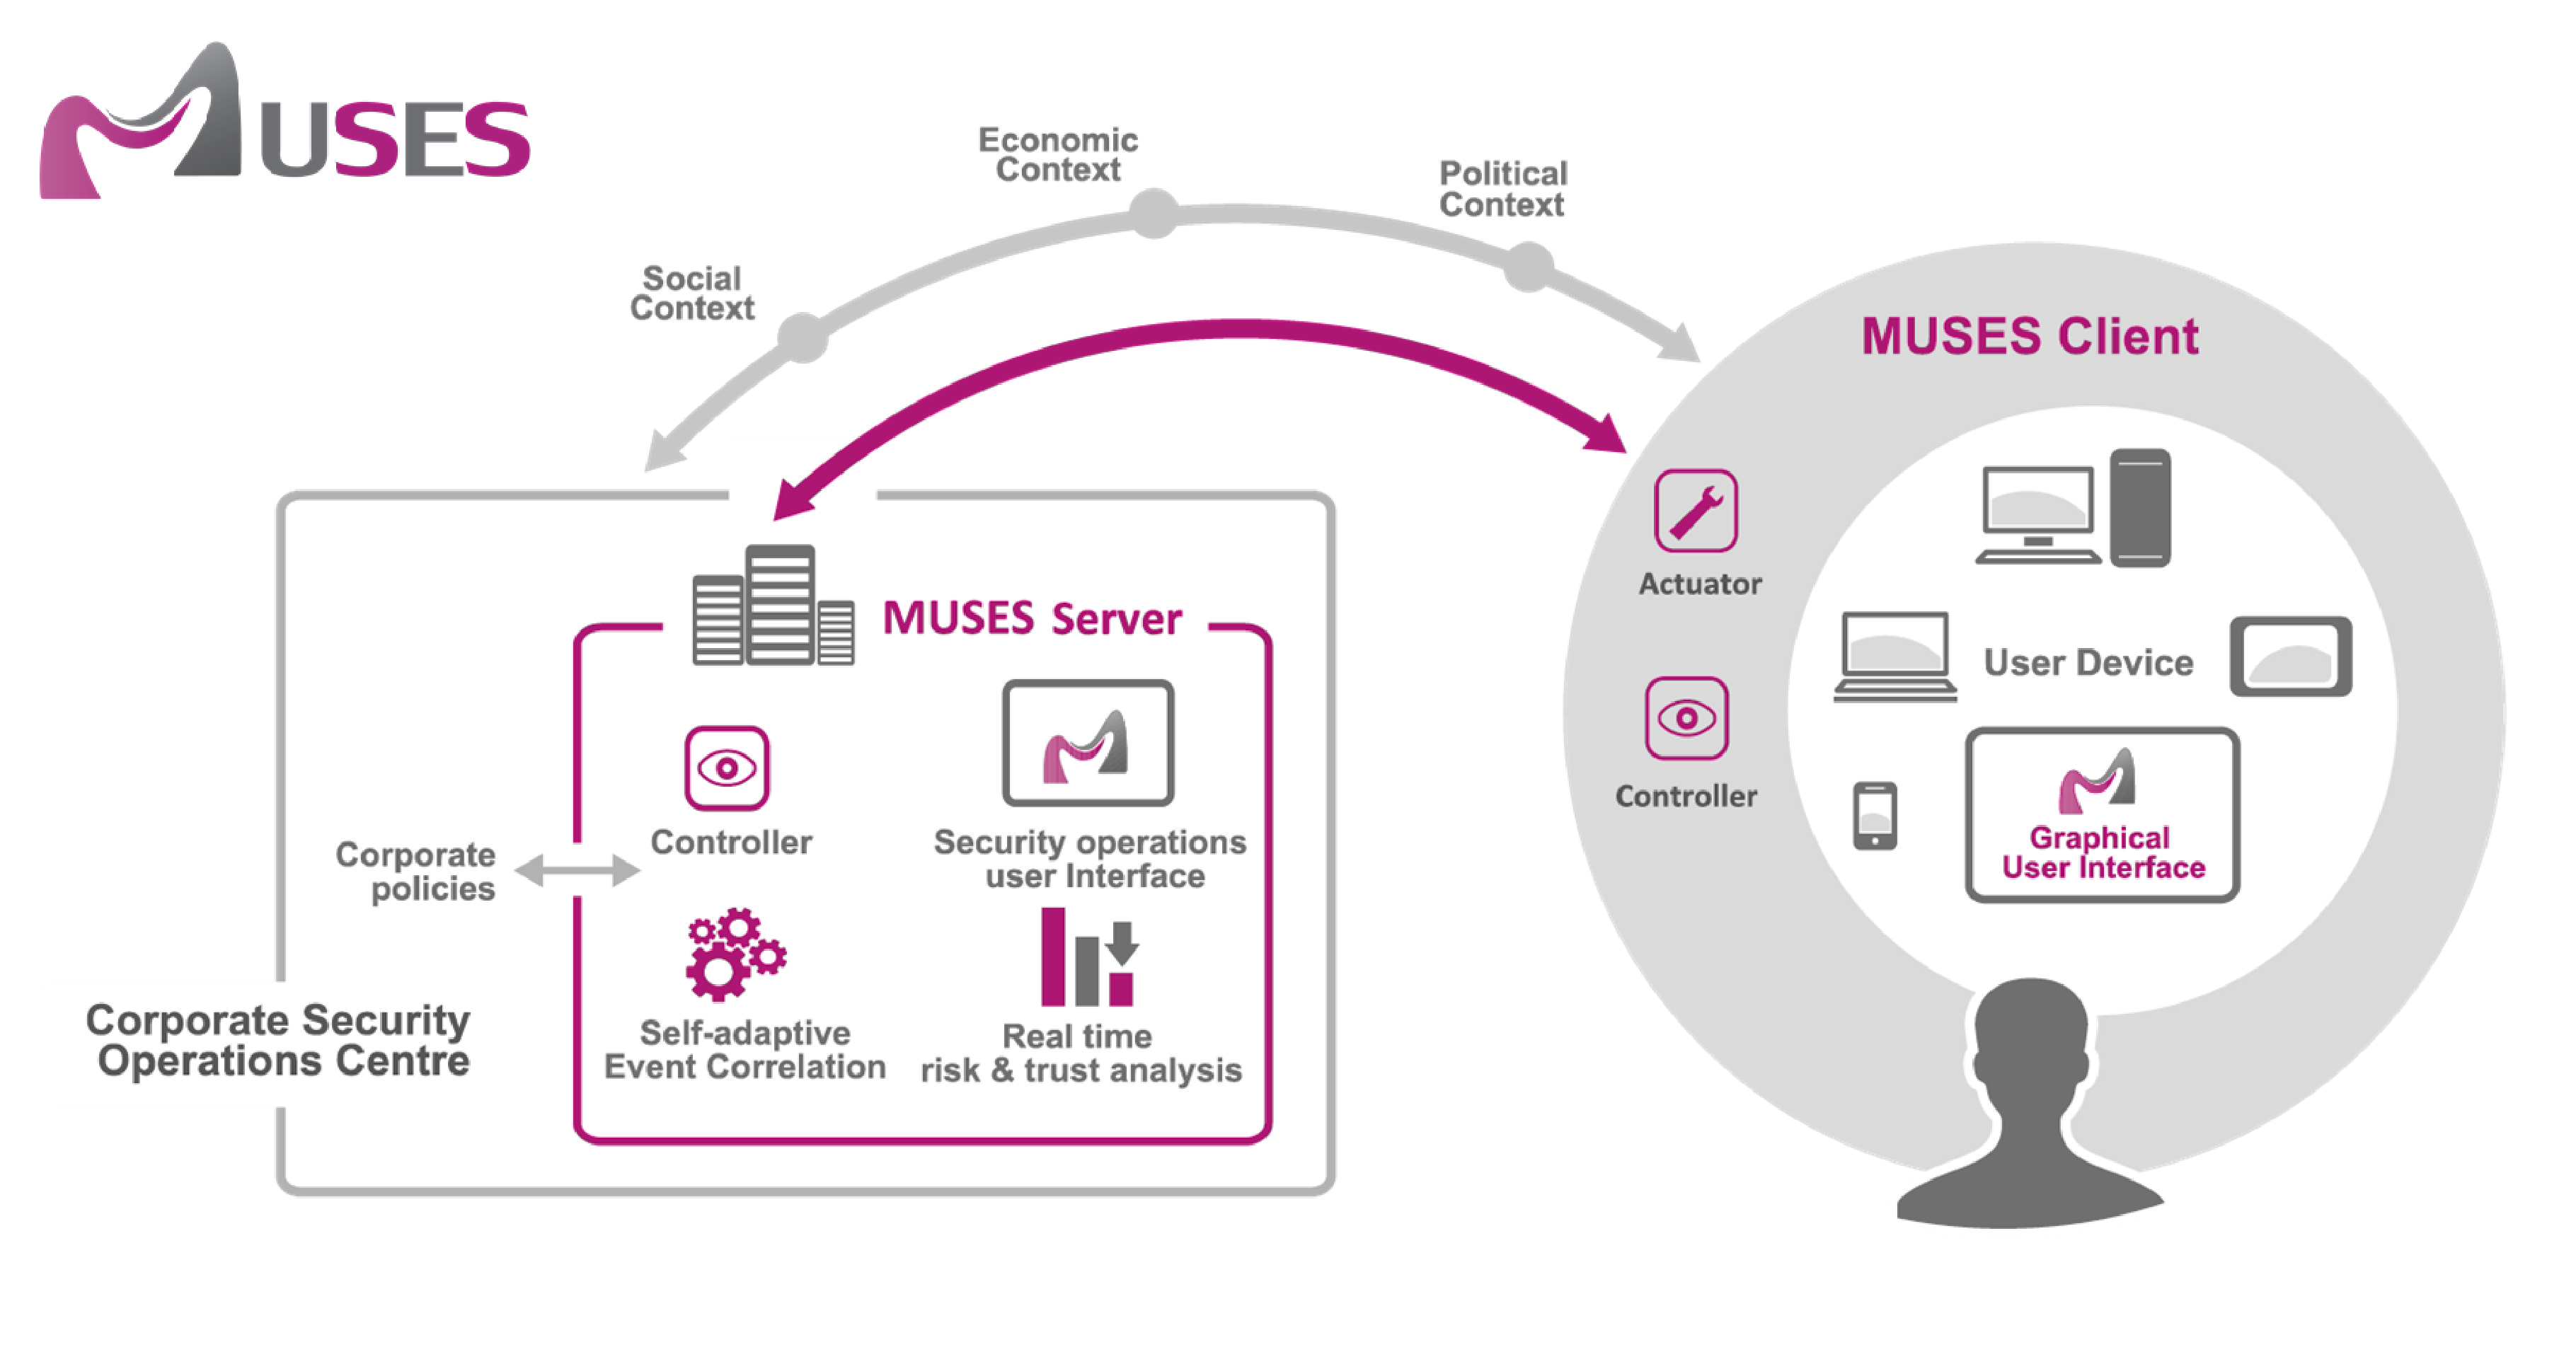
\includegraphics[scale =0.17] {gfx/byodSotA/system_overview.eps}
\caption{MUSES system overview. Conceptual model designed by S2 Grupo. \url{http://www.s2grupo.es/}}
\label{fig:system_overview}
\end{SCfigure}

As a summary, this application includes two modules: a \textit{controller} and an \textit{actuator}. The former consists of a number of implemented \textit{sensors} in the device, which monitor the environment and the users' behavior \footnote{Which has been introduced as the `context' of an event.}. Then, the user's actions, as well as device configuration, or connection properties, are translated into a sequence of events. These events, along with the stored patterns defining the user's conduct, are processed by the system in real-time by means of a Risk and Trust Analysis Engine (RT2AE) and an Event Correlation module. Then, a decision is taken in the corporate Security Operations Centre (SOC) side, considering the RT2AE output and the set of security rules adapted to that specific user and context. The corresponding feedback is communicated to the user through the \textit{actuator}, and then the user decides to comply or not with the policy. As mentioned before, MUSES depends on the MUSES Aware applications to be able to really stop the application if the risk is dangerously high. In case that MUSES cannot kill the application process, and if the user decides to continue performing a risky action, the user trust value will decrease and the CSO will be notified.

MUSES architecture is shown in Figure \ref{fig:architecture}. It is a \textit{client/server} approach in which the \textit{client} application can be installed in every user's mobile or portable device, independently of the platform. MUSES client is available up to date to be used in Android devices as well as in Windows mobile devices and PCs; the iOS client is under development. The same sensors are available in Android and Windows, but there is a strong limitation with monitoring iOS devices if they were not been \textit{jailbroken}. This means that if an iOS device has not been rooted, MUSES could not monitor every process in the device, and also it would have access only to some sensors. However, to be rooted is one of the situations that MUSES tries to avoid, which is why it depends on MUSES Aware apps. As far as the server is concerned, it has been developed using Java to be installed with an Apache Tomcat in the corporate server, independently of its OS. Both sides are connected through a secure channel using HTTPS over the Internet. Figure \ref{fig:architecture} only shows the high-level components in each part, along with the way the information flows in the system.

\begin{SCfigure}[tb]
\centering
 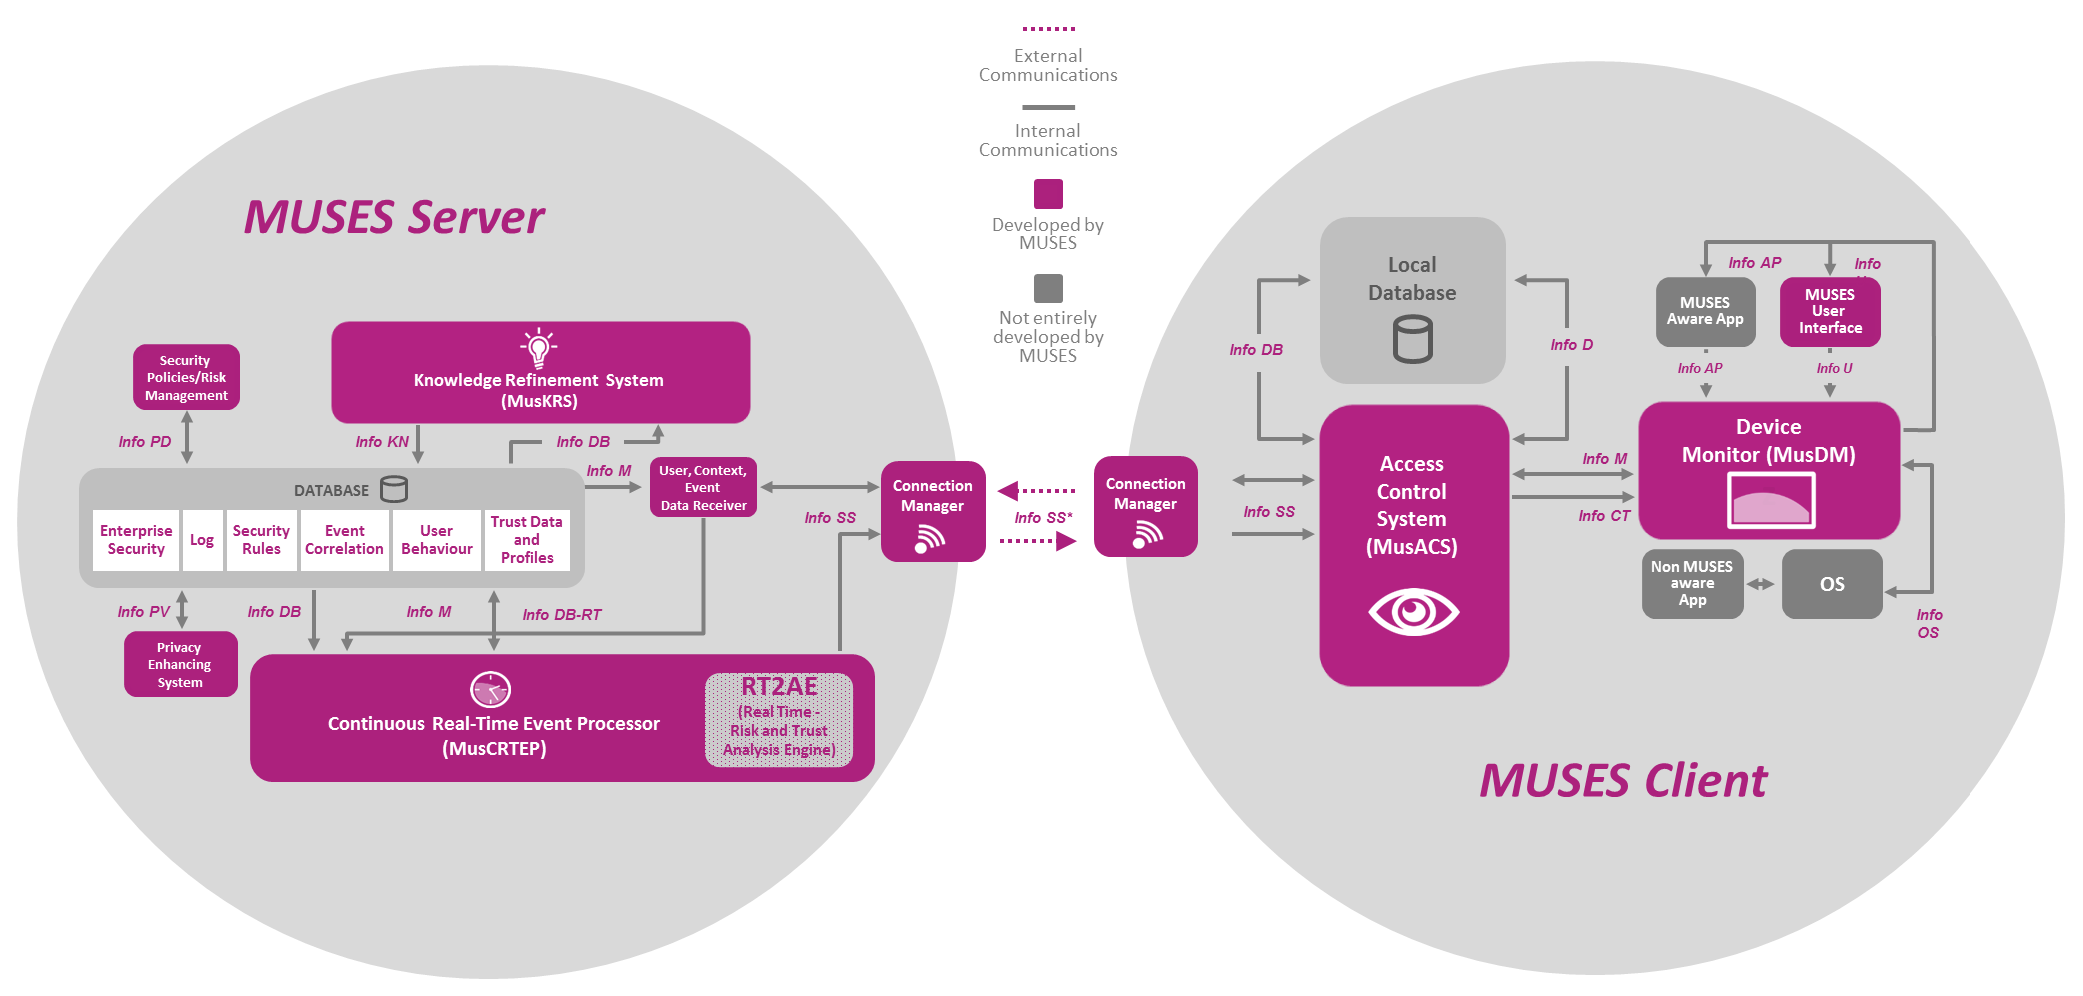
\includegraphics[scale =0.32] {gfx/byodSotA/architecture_modules.eps}
\caption{Design of the MUSES architecture (art by S2 Grupo).  \url{http://www.s2grupo.es/}}
\label{fig:architecture}
\end{SCfigure}

The use of a server is mainly based on the need of a powerful machine, able to work with massive amounts of data (\textit{Big Data}) \cite{BigData_11}, since the algorithms to apply to them require high computational costs \cite{Shirkhorshidi14Review}.
Moreover, part of the high computational cost methods to apply needs to be derived to this high-performance server, as the mobile devices do not count with enough computational power. These methods include DM \cite{DataMining_Lee01} and ML \cite{MachineLearning_Bishop06} techniques, which have been proved to be computationally expensive \cite{Cios07DataMining}. This server is also devoted to centralize the data gathering from all the devices in the company, composing a big database to which the commented techniques can be applied.

The system considers two working modes for every device: online and offline. In the \textit{online} mode the device can connect with the MUSES server, so that it can request the server to make a decision. On the other hand, in \textit{offline} mode the server cannot be reached by the device because there is not an available connection between them, so all the decisions are made locally.
This is done using an up-to-date copy on the Decision Table inside the Local database, which contains decisions for any type of detected event, along with the default actions to be performed if no rule is met. In this mode, the gathered information by the sensors in the device is stored for later submission to the server side when a connection is available, in order to be processed in the knowledge refinement process.
Moreover, when switching from offline to online mode, the device receives an updated copy of the Decision Rules, the so-called Device Policies, as a kind of antivirus database, in order to work again perfectly in offline mode if the connection is lost.

The MUSES system also performs an authentication process when the user logs in. The MUSES server authenticates to the MUSES client by means of a self-signed certificate. The authentication of the users is based on Spring Security, which is a Java EE framework that provides authentication, authorization and other security features for enterprise applications. When the user connects to the MUSES server for the first time, the MUSES client asks the server for the certificate, which is sent and installed in the client local database if the user credentials are right. As the user credentials are also stored in the MUSES client local database, the user can also log in to MUSES, and it therefore can apply the Device Policies. With regard to internal data security, MUSES makes use of the advantages that the OSs themselves offer to developers. More concretely, the first prototype for Android includes functionalities provided by the Android Application Sandbox \cite{blasing2010android}. This means that other applications cannot access MUSES data, nor even other developers. The only way to do this is by rooting the device, which is a state that MUSES can detect, and therefore warn about its implications. With regard to the encryption of the rest of the device data, MUSES stands for having a security policy which advices about the installation of existing open source tools, instead of having an own implementation.

% ----------------------------------------------------------

\section{Client/Device architecture}
\label{subsec:client}

There are three main components in this side:
\begin{itemize}
 	 \item \textit{Local Database}: it is a local security-based storage, which includes the set of security rules to be applied locally (Device Policies), user authentication data, and a cache of gathered events and information. The latter is useful when the device is in offline mode, so these events can be later submitted to the server side, when the device returns to online mode. It contains the so-called \textit{Decision Table}, a set of rules in which the antecedents are high-level events, and the consequents are the corresponding decisions/actions, namely `allow', `deny' or `request' (the decision must be made in the server side).
 	 \item \textit{Device Monitor (MusDM)}: module which contains the two main described modules, controller and actuator. When a user performs an action, an event is automatically created and either sent to the server (online) or locally stored (offline). In addition, there are several sensors implemented in the system which periodically scan different aspects of the device configuration and the environment. This way, the system acts equally over specific actions, as well as when it detects something from the sensors that is against the security policies.
 	 \item \textit{Access Control System (MusACS)}: module in charge of making the decisions considering the gathered data. These decisions can be made locally if possible, or can be requested to the server if there is no rule which matches with the occurred events. 
 	 
 	 The subcomponents are the \textit{Decision Maker}, which performs the decision process; the \textit{User, Context, Event Handler}, which processes the events and information to be used for making the decision or stored for further submission (depending on the mode and on the gathered data); and the \textit{Security Policy Receiver} that updates the set of decisions (or Device Policies) in the Decision Table with those received from the server side, after an update or decision process.
\end{itemize}

The client is an important part of the a-priori risk treatment, because it both monitors the whole context, and finally acts or warns the user in the event of a security violation. 
But security violations are mainly identified by security rules, which is why MUSES needs at least an initial set of rules, defined by the CSO. Then, it makes use of DM and CI techniques to improve or optimize them, enhancing the coverage. 
That is to say, the more sensors are implemented, the more information related to event context can be extracted. Implementing a sensor means to include a programmed method which triggers MUSES to start `listening' to some parts of a device. Then, the initial security rules establish which situations might cause a security violation, and the sensors provide with information which helps the MUSES server to identify events that are alike to the ones that are already known as dangerous.

MUSES implements the following monitoring sensors:

\begin{description}
  \item[Connectivity sensor:] It gathers all information related to network communications, in addition to security properties like network encryption, or number of neighbours. This allows MUSES actuator to forbid the user for sending important emails, or opening key assets if, for instance, the network encryption is not secure enough. 
  \item[Device protection sensor:] Which scans device security settings, such as the time until the device screen turns off, if the device has the screen protected with a password, or if the device is rooted \cite{hildenbrand2014}. This security mechanism adds the possibility of detecting security violations even if the user is not doing a specific action.
  \item[Location sensor:] User location can be obtained using the device GPS. Although, this might be taken against the preservation of user privacy. This is why MUSES allows the definition of a number of `zones', and therefore it only checks if the user is inside them or not, acting in consequence.
  \item[Mail sensor:] If the user is writing an email, MUSES client sensor can also check the email attributes. Thus, it can detect if the event context is dangerous, according to security policies and the RT2AE, before the mail is sent.
  \item[File sensor:] The type of file, also called \textit{asset}, is also very important for the application of security rules. Thus, this sensor aims to detect if some files might need more strict security policies, also depending on the rest of sensors.
  \item[App sensor:] It is in charge of monitoring the information about the application from which the user is performing the action, but also looks for installed trusted antivirus, and encryption applications. Additionally, this sensor gathers information about the applications which the user tries to install or uninstall.
\end{description}

It is important to note that MUSES does not work as an antivirus itself, but has a sensor which checks if the device has already an antivirus, and raises a security violation alert if not. It might happen then that the user ignores this advice and the device becomes compromised. As it would be explained in the next section, the sensors are constantly sending their monitored values, and therefore patterns are created, stored, and processed on the server. In case the device gets infected with rootkit-type malware \cite{bickford2010rootkits}, a sudden change in the values of the sensors will mean a significant change in the patterns. Then, this change in the patterns will be noticed by the server, which will immediately warn the user, and decrease the device trust value.

The rest of the components shown in the figure are: the \textit{MUSES User Interface (UI)}, the application through which the user interacts with the system; and the \textit{Connection Manager}, which controls the communications between MUSES client and MUSES server. 
In addition, there are two types of applications considered in this system. On the one hand, the \textit{MUSES Aware App} is an application adapted to MUSES, so the system can directly interact with it. This application must be implemented using the MUSES API (Application Program Interface). It should be noted that MUSES is an application that is running in the background, and third party apps can communicate with MUSES and ask for a response. Then, the MUSES API is not a normal API for building the third party application, but a collection of methods to allow this communication\footnote{The MUSES API is defined in the project, so for every application desired to be MUSES Aware, it should be implemented using this.}.
The main advantage of having MUSES Aware applications, is because actuator is able to actually forbid the users for doing something, if it implies a big risk for the company.

On the other hand, the \textit{Non MUSES Aware Apps} are those which MUSES cannot directly interact with. Usually, they can be accessed through the OS. But the type of information to gather from them and also the type of actions to do over them strongly vary depending on the OS, which should not be modified according to  \cite{Gessner13userfriendly}.
As was already mentioned, when MUSES is not able to close the application, a pop-up feedback message is automatically shown to the user. This message informs about why the action is considered as risky and what the user can do to avoid it.

% ----------------------------------------------------------

\section{Server architecture}

As in the client, we describe the three main components:
\begin{itemize}
	 \item \textit{System Database}: it stores all the information that the system can manage, including authentication data, enterprise security policies, values of the assets, user-related information (trust, context), events data, and, of course, security rules to apply with regard to the security policies.

	 \item \textit{Continuous Real-Time Event Processor (MusCRTEP)}: this component is the core of the MUSES system with respect to the decision making process. It includes an \textit{Event Processor}, the module in charge of performing the event correlation process \cite{deliverable21, deliverable52}. This is done by a so-called `Event correlation engine', which is in charge of taking the user action events that are sent from the device client, and analyzing them to look for an existing security rule that could be applied to the situation. The engine discovers that by analyzing the context events which are sent with the user action event, so that a complete model of the risks can be built. The output of this module is an `access request' which is sent to the \textit{RT2AE}. It considers the information included in the access request, as well as other information such as trust data and profiles, values of the assets, user reputation, or opportunity, to perform a risk and trust analysis task \cite{RT2AE_SOTICS13}. Finally, the RT2AE extracts the set of potential rules to consider in the analyzed situation, and these rules are therefore transformed into decisions (or Device Policies) and submitted to those devices to which they apply.

	 \item \textit{Knowledge Refinement System (MusKRS)}: this module is in charge of analyzing the information stored in the system database by means of Data Mining techniques, identifying relevant data, such as important patterns, key features, or security incidents. These are later processed for tuning up the existing set of rules, or for inferring new ones. The MusKRS component, along with the MusCRTEP, are what represent the extension of the state of the art in security solutions for a BYOD environment. 

\end{itemize}

There are some other components, which add extra functionalities to the system, namely:

\begin{itemize}
  \item A \textit{Security Policies/Risk Management} tool, that lets the company CSO to define and manage Security Policies and Rules in a friendly way. It also lets the management of risk-related information, useful for the RT2AE process, such as the values of the assets.
  \item  The \textit{Privacy Enhancing System}, which is a module aimed to fit with the legal compliance of the system regarding the user's data anonymization and retaining of these data in the system. There are three important points with relation to this matter \cite{deliverable72}. First, the data that the user provides to the system, such as name, or email, is only used for authentication purposes, so they are checked when the user logs in the system, but they are not used for Data Mining tasks. Then, the location of the device is never sent and stored in the database, but as stated in the previous section, there are a number of defined `zones'. What is checked is that the user is inside one of those zones of interest. For instance, a company might want to know if the user is inside or outside a zone defined as `company premises'. And finally, the use in MUSES of what is called as `soft limit' and `hard limit' \cite{deliverable72}. These limits exist to ensure the users that their data will not be kept longer than necessary. The soft limit is defined by the components that use the data (Event Processor, RT2AE, and Knowledge Refinement System) for decision making or rule refinement, but do not need that data anymore. In addition, the hard limit is provided by the law, in case that the employee leaves the company, or if there is a national law specifying a maximum data retention period.
  \item \textit{User, Context, Event Data Receiver}, which is devoted to receive data from the device side, such as events, or user-related data, and to distribute them among the components, storing in the database, and requesting the Event Processor to start the correlation task. Finally, there is another \textit{Connection Manager} which controls the communications with the device side. 
\end{itemize}


% ----------------------------------------------------------

\section{Self-Adaptation in MUSES: The Knowledge Refinement System}

The self-adaptation, to the user and context, of the set of Corporate Security Rules is one of the main features of the MUSES system.
To this end, the \textit{MusKRS} module is in charge of analyzing all the gathered events, context, and user-related data. Then it processes the data and adapts or refines the security rules. This refinement is meant as an improvement of the existing security rules, and its aim is to deal with new, possibly insecure, events. As a result, a set of optimizations and additions to the set of security rules are proposed to the CSO of the company.

This procedure is composed by two main steps: first, a DM \cite{DataMining_Lee01} + ML \cite{MachineLearning_Bishop06} process is performed in the \textit{Data Miner} sub-component; second, a refinement and inference process is done in the \textit{Knowledge Compiler} sub-component, using the data that was extracted in the first step, and by means of CI techniques.
The refinement or adaptation of the security rules can be made through techniques as simpler as generalization or specialization of rules, for instance, or by more complex CI methods such as Evolutionary Algorithms \cite{EAs_Back96}.

Another important fact is that MUSES functionalities are completed by a human controller, normally the CSO, who supervises the system activity by means of a graphic interface they can interact with.
Thus, adapted and inferred security rules are not directly added to the current set of rules, but they are proposed instead as draft rules to this human controller, in order to be accepted if they are interesting and useful. The system also uses the acceptance or rejection of new rules as `feedback`, learning from these decisions, and refining the rules according to this.

The following sections describe these processes: first, focusing on DM techniques to be used both automatically by the MusKRS, and by the mentioned graphic interface for showing useful information to the CSO; second, used CI techniques are explained, mainly focusing in Evolutionary Computation (EC) \cite{EAs_Back96} approaches. EC methods have demonstrated to have a good performance, and have been widely used in security-based environments for solving security issues, such as intrusion detection \cite{GA_intrusion-majeed}, design and evaluation of security protocols \cite{GP_intrusion-lu,GA_networksecurity-zarza}, or for the optimization of different aspects related with security: IT security costs \cite{EAs_securitycosts-kirta}, and cryptographic protocols \cite{GA_cryptographicprotocols-zarza2}, among others.

% ------------------------------------------------------------------
%
\subsection{Data Mining + Machine Learning}
\label{subsubsec:dm_ml}

This task is performed by the \textit{Data Miner} module. It  takes the `raw' data from the database and processes the information, in order to yield a set of relevant data for the Knowledge Compiler module and for the human controller. In the first case, this Data Miner component takes the set of data as a reference for refining or adapting the current set of security rules, to deal with anomalous situations, for instance.

The set of data is composed by the so-called patterns, which consist of an occurred event and all the related information to that event. This means that the context in which the event was, is translated into a number of \textit{attributes} of the pattern. Moreover, a lot of attributes are extracted from the events, for obtaining the more information as possible. 
During the first trials, a mean of 201 events per day and user was observed. By considering just a medium size company, of 250 employees, that would make an average of 50300 events per day, of which a high number of features are extracted. Furthermore, if for instance 6 months are considered for the `hard limit' (see previous section), the amount of events to be processed would exponentially grow, until reaching the 9 million events. For even bigger companies, this all result in huge datasets, so that MUSES makes use of several Big Data processing methods \cite{BigData_11}, such as: 

\begin{itemize}

\item \textit{Pattern Mining} \cite{PatternMining_Han07}: 
From the whole set of patterns which form the built dataset, the most frequent, as well as the uncommon, are obtained. The idea is that infrequent patterns are potentially suspicious, and thus, could be of interest to be checked by the CSO, or to serve as a reference for the rule-refinement process.

\item \textit{Classification} \cite{classification_67}: 
This technique tries to train a model (classifier) able to associate every pattern in the dataset to a class, so that the model could be used for assigning a class for further incoming patterns with an unknown category.
Then, the model learns from events that, according to the ISPs, had been previously marked as `allowed' or `denied'. When a new event arrives to the server, if it has not an assigned decision, the classifier should provide one based on the similarity with previous, and already labeled, patterns.

\item \textit{Clustering} \cite{Clustering_Jain99}: 
The aim of this method is grouping the patterns considering some similarity criteria, in order to manage them as a set. This is used for providing data visualization mechanisms through a graphical interface. This would make easier to interpret data interaction and the distribution in clusters with respect to the different attributes, or features, of the patterns.

\item \textit{Feature Selection} \cite{FeatureSelection_Guyon03}: 
It consists of extracting the most important variables from the data. Feature selection techniques have been proven \cite{liu1998feature} to preserve the quality of the original feature set in terms of classification accuracies, while significantly improve the processing time.

\item \textit{Data Analysis}: 
This provides the CSO with mechanisms to visualize interesting facts about the data, such as most frequent events, dangerous or suspicious users according to their behavior, most triggered rules, etc. All this information is shown to the CSO via the mentioned graphical interface, implemented in the server.

\end{itemize}

%\pagebreak

% ------------------------------------------------------------------
%
\subsection{Computational Intelligence: Evolutionary Computation Methods}
\label{subsec:ci}


MUSES uses different EC approaches, initially, two in the DM/ML part of the process, and three in the rule-refinement and adaptation phase. They are based on Genetic Programming (GP) \cite{GP_Koza92}, and Genetic Algorithms (GAs) \cite{GAs_Goldberg89}.

The Data Miner module adopts two evolutionary-based approaches. In the first place, a \textit{GP-based classification} method. This is useful for two main reasons: to deal with the data class imbalance \cite{imbalance_techniques_02}, which is very common in classification problems with real systems, gathering real data; and to better manage categorical data, since most of the features and information gathered from the events take these kind of values.

Thus, this kind of classification method is able to manage unbalanced datasets, for instance, by considering a fitness function in which a cost is associated with the classifier accuracy at every iteration, having a penalty cost when the classifier makes a false negative. A false negative is an element from the minority class which is classified as belonging to the majority class \cite{cost_adjustment_07}.
With regard to the type of data, since GP algorithms can manage rule or tree based models, it works perfectly with any categorical feature, yielding a good classifier as it has been demonstrated in \cite{cost_adjustment_07}.

The second evolutionary approach taken in the Data Miner is the Feature Selection process that was mentioned in the previous section. This process is conducted using a GA as a meta-algorithm to test all the possible combinations of pattern features in the classification. Thus, the GA algorithm can optimize the group of features to be considered in the classification task, improving both the computational time of this task and also the obtained accuracy of the method \cite{liu1998feature}.

On the other hand, the refinement or adaptation of the security rules is performed by the \textit{Knowledge Compiler} module, and it uses three EC methods. These methods can be used for inference and optimization, and they use different data as part of the process, such as:

\begin{itemize}

\item The information extracted from the Data Miner sub-component, mainly concerning the anomalous, unclassified or misclassified patterns. These are those patterns which did not match with any of the existing classes, as they are quite different from the patterns belonging to those classes. This way, they cannot be included in any of the classes and thus they should be taken into account for a potential inference or update in the set of security rules, in order to `cover' them.

\item User-related information, and context information in general, corresponding to those anomalous or unlabeled events. Thus, the user's location zone, role, or device settings, for instance, can be considered in order to select the applicable set of rules for those conditions.

\item Risk information extracted from the user profile, e.g. ``Did the user received a lot of `denies' or `allows' before?'', in other words, ``Is the user trustworthy?''. In case the user is not, meaning that the user trust value is low, more restrictive rules can be created, otherwise the corresponding rules could be `softer' for that user.

\item The information about the user behavior with respect to system messages, whether the users acts in consequence or against MUSES advice, as well as user feedback. The user feedback has been measured in the MUSES trials by making interviews with the people who have used MUSES, but it can also be measured by pop-up messages, such as ``has this information been useful?''.
All this information contributes to the inference of new rules or in adaptation, in order to deal with, for instance, users that repeatedly ignored warning messages.
Moreover, important log information with regard to the parameters used or the decisions made in the different modules can be used for further tests of new inferred rules, as it is explained below.

\end{itemize}

As the rule refinement process is considered of the same importance as inferring new ones, the following three approaches have been implemented:

\begin{itemize}

\item A \textit{GP rule inference} method, which generates new rules in order to `cover' those situations that have been not contemplated in the current set of rules. Thus, a new rule would be created for dealing with the patterns to which the classifier could not assign a class.
The generation of new rules is done by considering the so-called \textit{dictionary}, i.e. a set of terms corresponding to all the possible context situations and user actions in the system, which are the antecedents and consequents \footnote{The antecedents are the conditions of a rule that have to be met to apply the consequents.} of the security rules to be inferred.
The evaluation of these rules is done by considering the information that has been described. Thus, it is possible to `simulate' the whole system behavior when the new rule is included. Therefore, the system gets a value of its performance in terms of, for instance, how many of the events that were not classified or misclassified, are covered now. As was also mentioned, the user or device trust values influence the creation of the rules.
Finally, the inferred rules are proposed to the CSO as ``new, but not yet refined'', along with their evaluated performance.

\item A \textit{GP rule refinement} approach, which optimizes the current set of rules, adjusting the values in the conditions. The set of rules that could be refined is composed by the new rules from the GP-based inference, but also by the original set of rules which was already completed by the Data Miner. Thus, some superfluous parts of the rules and even complete rules could be removed or improved, obtaining for instance specializations or generalizations of existing rules which could lead to a better performance. The evaluation of the whole set of security rules is done by considering the number of unlabelled patterns that are `covered' after the adjustments. Again, the rules at the end of this step are presented to the CSO as ``refined''. The CSO is the one who decides, according to the performance simulation results, if an inferred rule, or the refined one, is the rule which is finally included in the system.

\item A \textit{GA optimization} algorithm for adapting the values of the assets. These are numerical representations of the importance of the corporate assets, and are considered in the Real-Time Risk and Trust Analysis process, in order to assign a risk value to every potential decision that can be made by the system.
By evaluating the partial solutions proposed by the GA, this approach provides the CSO, who is in charge of assigning and adjusting these values over time, with information about the most dangerous situations for certain assets. In this process, then, the context information that is gathered by the system is very important. The adaptation or adjustment concerns the change in the value that an asset has due to a loss of importance, for instance, for being an out-to-date document.

\end{itemize}

As a summary, the Knowledge Compiler module uses two EC-based processes for inferring and refining rules, plus another one for adjusting values of the assets. Both the inferred rules and the refined rules are presented to the CSO, who includes them or not in the system, and this acceptance or rejection acts itself as a feedback for future rule inference.


% ---------------------------------------------------

\section{Trials and tests of MUSES}
\label{subsec:trials}

A MUSES first prototype, implemented for Android devices, has been recently tested. These trials have been conducted in an actual Spanish company, with 50 employees using the system on their own devices.
The trials were divided in two phases: \textit{silent} and \textit{verbose}, 1 month duration each. During the \textit{silent} phase, MUSES was able to gather data, but without warning the users when a security incident was happening. A total of 23358 security violations were detected. In the \textit{verbose} stage, MUSES started to show warning pop-ups to the users, every time a security incident happened. 

As results, not only the number of security violations were reduced by half in the first two weeks (10977), but the number went on decreasing until it was 0 even before the trials period finished. Thus, we can assume that MUSES is an effective tool, even though it has the limitation of needing an initial set of defined security rules to start working (this will be better explained in Section \ref{sec:comparison}). For this, MUSES also includes a set of guidelines for the companies to build adequate security policies. For instance, the set of initially defined rules used for the trials included a blacklist of forbidden applications, a whitelist of allowed ones, and requirement of antivirus, among others.

With respect to the computational costs, in this first prototype it takes less than 0.5 seconds in the client side, if there is already a decision in the local table for the happened event. Otherwise, i.e. if there is need to ask the server to make a decision (by means of Event Correlation + Risk and Trust Analysis), the time grows up to 2.5 seconds in the worst case.
%\include{Chapters/appendixosgiliath}
%\include{Chapters/apendiceC}
%********************************************************************
% Other Stuff in the Back
%*******************************************************
\cleardoublepage
%********************************************************************
% Bibliography
%*******************************************************
% work-around to have small caps also here in the headline
\manualmark
\markboth{\spacedlowsmallcaps{\bibname}}{\spacedlowsmallcaps{\bibname}} % work-around to have small caps also
%\phantomsection
\refstepcounter{dummy}
\addtocontents{toc}{\protect\vspace{\beforebibskip}} % to have the bib a bit from the rest in the toc
\addcontentsline{toc}{chapter}{\tocEntry{\bibname}}
%\bibliographystyle{plainnat}
\bibliographystyle{babplain-fl}
\label{app:bibliography}
\bibliography{tesis,review_muses,data_mining_urls,GPrules}
%\cleardoublepage
%\include{FrontBackmatter/Declaration}
\cleardoublepage
%La contraportada tiene que estar en p�gina par!!
% \include{FrontBackmatter/DirtyBackpage}

% ********************************************************************
% Game Over: Restart, Restore or Quit?
%*******************************************************
\end{document}
% ********************************************************************
